% !TEX program = xelatex
\documentclass[12pt, a4paper, oneside]{report}

% ════════════════════════════════════════════════════════════════════
%  PREAMBLE — GNN EGFR Inhibitor Discovery Thesis
%  Department of Mathematics, IoST, Tribhuvan University
%  APA 7th Edition | 1.5 line spacing | Times New Roman
%
%  ENGINE : XeLaTeX  (required for Nepali Unicode / Kalimati font)
%  COMPILE: xelatex → biber → xelatex → xelatex
%           OR:  latexmk -xelatex main.tex
% ════════════════════════════════════════════════════════════════════


% ── Page layout ──────────────────────────────────────────────────────
% IoST margins: top/bottom/right = 1 in, left = 1.5 in (binding)
\usepackage[top=1in, bottom=1in, right=1in, left=1.5in]{geometry}

% ── Fonts (XeLaTeX) ──────────────────────────────────────────────────
\usepackage{fontspec}

% Main English font
\setmainfont{Times New Roman}[
  BoldFont       = Times New Roman Bold,
  ItalicFont     = Times New Roman Italic,
  BoldItalicFont = Times New Roman Bold Italic,
]

% Math font — now properly installed
\usepackage{unicode-math}
\setmathfont{latinmodern-math.otf}



% Nepali font (Kalimati still missing)
\newfontfamily\nepalifont{Kohinoor Devanagari}[Script=Devanagari]
% Fallback if Noto is also missing:
% \newfontfamily\nepalifont{FreeSerif}[Script=Devanagari]

% Optional: If Latin Modern Math still complains, try this exact filename
% \setmathfont{latinmodern-math.otf}


% ── Line spacing ─────────────────────────────────────────────────────
\usepackage{setspace}
\onehalfspacing


% ── Mathematics ──────────────────────────────────────────────────────
\usepackage{amsmath}
\usepackage{float}
% NOTE: do NOT load amssymb or amsfonts — unicode-math already provides
%       \mathbb, \mathcal, etc. and will conflict with them.


% ── Tables ───────────────────────────────────────────────────────────
\usepackage{booktabs}       % \toprule \midrule \bottomrule
\usepackage{longtable}      % tables spanning multiple pages
\usepackage{multirow}       % \multirow — merged row cells
\usepackage{tabularx}       % auto-width X columns
\usepackage{array}          % extended column types
\usepackage{multicol}       % multi-column layout
\usepackage{pifont}         % checkmark/cross symbols

% ── Sequential Table/Figure numbering (IoST §10.7d) ──────────────────
% Regulation requires Table 1, Table 2, … and Figure 1, Figure 2, …
% numbered sequentially THROUGHOUT the thesis (not chapter-based 2.1).
% \counterwithout is a LaTeX kernel command (since 2018); no package needed.
\counterwithout{table}{chapter}
\counterwithout{figure}{chapter}
% Equations numbered (1), (2), … sequentially throughout the thesis (IoST §10.8)
\counterwithout{equation}{chapter}





% ── TikZ (pipeline / architecture diagrams) ──────────────────────────
\usepackage{tikz}
\usetikzlibrary{shapes.geometric, arrows.meta, positioning,
                fit, backgrounds, calc}




% ── Colors ───────────────────────────────────────────────────────────
\usepackage[table, xcdraw]{xcolor}
\definecolor{tableblue} {RGB}{210, 228, 255}
\definecolor{headerblue}{RGB}{ 68, 114, 196}


% ── Hyperlinks ───────────────────────────────────────────────────────
% colorlinks=true with all colors black satisfies IoST print requirement
% Load BEFORE cleveref
\usepackage[colorlinks=true,
            linkcolor=black,
            citecolor=black,
            urlcolor=black,
            bookmarks=true]{hyperref}

% PDF metadata — fill in before final submission
\hypersetup{
  pdftitle   = {Graph Neural Networks for the Classification and Lead
                Identification of EGFR Inhibitors in Non-Small Cell
                Lung Cancer},
  pdfauthor  = {Krishna Gaire},
  pdfsubject = {M.Sc.\ Data Science Thesis, Tribhuvan University},
  pdfkeywords= {GNN, EGFR, NSCLC, AttentiveFP, Drug Discovery},
}

% ── Bibliography (APA 7th — IoST mandated) ───────────────────────────
% Load AFTER hyperref
\usepackage[backend=biber,
            style=apa,
            sorting=nyt,
            maxcitenames=2,
            uniquelist=false]{biblatex}
\addbibresource{references.bib}


% ── Typography ───────────────────────────────────────────────────────
% Under XeLaTeX: protrusion only (no expansion), still reduces
% overfull boxes at right margin.
\usepackage{microtype}
\setlength{\emergencystretch}{2em}   % last-resort overflow guard


% ── List formatting ──────────────────────────────────────────────────
\usepackage{enumitem}    % \begin{itemize}[noitemsep], etc.


% ── Page rotation ────────────────────────────────────────────────────
\usepackage{rotating}    % \begin{sidewaysfigure / sidewaystable}
\usepackage{pdflscape}   % full landscape pages
\usepackage{afterpage}   % \afterpage{\clearpage}




% ── URL line-breaking ────────────────────────────────────────────────
\usepackage{url}
\def\UrlBreaks{\do\/\do-\do_\do.\do=}
\usepackage{xurl}        % also allows breaks at more characters


% ── csquotes (required by biblatex) ─────────────────────────────────
\usepackage{csquotes}


% ── TOC formatting ───────────────────────────────────────────────────
\usepackage{tocloft}
\renewcommand{\cftchapfont}     {\bfseries}
\renewcommand{\cftchappagefont} {\bfseries}
\setlength{\cftchapindent}     {0pt}
\setlength{\cftbeforesecskip}  {4pt}
\setlength{\cftsecindent}      {1.5em}
\setlength{\cftsubsecindent}   {3.5em}
\setlength{\cftsubsubsecindent}{5.5em}
\setcounter{tocdepth}    {3}
\setcounter{secnumdepth} {3}

% List of Tables / Figures entries as "Table 1: caption" / "Figure 1: caption"
% with the "Table N:" / "Figure N:" prefix in bold (IoST Appendix K/L sample).
\renewcommand{\cfttabpresnum}{\bfseries Table\ }
\renewcommand{\cfttabaftersnum}{\bfseries :\mdseries}
\renewcommand{\cfttabnumwidth}{5.2em}
\renewcommand{\cftfigpresnum}{\bfseries Figure\ }
\renewcommand{\cftfigaftersnum}{\bfseries :\mdseries}
\renewcommand{\cftfignumwidth}{5.6em}


% ── Paragraph spacing ────────────────────────────────────────────────
\setlength{\parindent}{0pt}
\setlength{\parskip}  {6pt}
\clubpenalty  = 10000
\widowpenalty = 10000


% ── Section heading format (IoST style) ──────────────────────────────
\usepackage{titlesec}

\titleformat{\chapter}[display]
  {\normalfont\fontsize{14}{16}\bfseries\centering}
  {\fontsize{14}{16}\selectfont Chapter~\thechapter}
  {0pt}
  {\fontsize{14}{16}\bfseries\centering}
\titlespacing*{\chapter}{0pt}{20pt}{20pt}

\titleformat{\section}
  {\normalfont\fontsize{12}{15}\bfseries}{\thesection}{1em}{}
\titlespacing*{\section}{0pt}{14pt}{8pt}

\titleformat{\subsection}
  {\normalfont\fontsize{12}{14}\bfseries}{\thesubsection}{1em}{}
\titlespacing*{\subsection}{0pt}{12pt}{6pt}

\titleformat{\subsubsection}
  {\normalfont\fontsize{12}{14}\bfseries}{\thesubsubsection}{1em}{}
\titlespacing*{\subsubsection}{0pt}{10pt}{4pt}


% ── Page style ───────────────────────────────────────────────────────
% IoST: page number centred at bottom; no running header
\usepackage{fancyhdr}
\pagestyle{fancy}
\fancyhf{}
\fancyfoot[C]{\fontsize{10}{12}\selectfont\thepage}
\renewcommand{\headrulewidth}{0pt}
\renewcommand{\footrulewidth}{0pt}

\fancypagestyle{plain}{%
  \fancyhf{}%
  \fancyfoot[C]{\fontsize{10}{12}\selectfont\thepage}%
  \renewcommand{\headrulewidth}{0pt}%
  \renewcommand{\footrulewidth}{0pt}%
}


% ── Convenience symbols ──────────────────────────────────────────────
\newcommand{\cmark}{\ding{51}}   % ✓  checkmark
\newcommand{\xmark}{\ding{55}}   % ✗  cross


% ── Figure search path ───────────────────────────────────────────────
\graphicspath{{figures/}}


% ════════════════════════════════════════════════════════════════════
%  DOCUMENT
% ════════════════════════════════════════════════════════════════════
\begin{document}

% ----------------------------------------------------------------
%  Front matter — roman pagination
%  TU IoST Research Regulation 2025, §10.1
% ----------------------------------------------------------------

% IoST §10.4(d): front matter uses Roman numerals; the title (cover) page is
% counted as page i but the number is NOT printed; the inner cover number is
% also NOT printed. Printed Roman numbering becomes visible from the Declaration.
\pagenumbering{roman}

% Front-matter section headings (Abstract, List of …, Table of Contents) at
% 16pt per IoST appendix specifications. Restored to 14pt before Chapter 1.
\titleformat{\chapter}[display]
  {\normalfont\fontsize{16}{18}\bfseries\centering}
  {\fontsize{16}{18}\selectfont Chapter~\thechapter}{0pt}
  {\fontsize{16}{18}\bfseries\centering}

%% Cover Page (outer cover — unnumbered, not counted)
% ════════════════════════════════════════════════════════════════════
%  front_pages/3_innercoverpage.tex
%  TU IoST Thesis Inner Cover Page — Appendix B Format
% ════════════════════════════════════════════════════════════════════

\newpage
\thispagestyle{empty}
\singlespacing
\begin{center}

\vspace*{0.3in}

% ── 1. TITLE ─────────────────────────────────────────────────────────
{\fontsize{18}{22}\selectfont\textbf{%
Graph Neural Networks for the Classification And Lead\\[3pt]
Identification of EGFR Inhibitors in Non-Small Cell\\[3pt]
Lung Cancer%
}}

\vspace{0.25in}

% ── 2. LOGO ──────────────────────────────────────────────────────────

\includegraphics[width=2in, height=2in, keepaspectratio]{figures/TU_logo.png}

\vspace{0.25in}

% ── 3. DEGREE STATEMENT ──────────────────────────────────────────────
{\fontsize{14}{18}\selectfont\textbf{%
A Thesis Submitted for the Partial Fulfillment of the\\[3pt]
Requirements for the Master of Science (M. Sc.)\\[3pt]
Degree in Data Science%
}}

\vspace{0.25in}

% ── 4. SUBMITTED TO ──────────────────────────────────────────────────
{\fontsize{14}{18}\selectfont\textbf{Submitted to the}}\\[4pt]
{\fontsize{14}{18}\selectfont\textbf{Central Department of Mathematics /}}\\[4pt]
{\fontsize{14}{18}\selectfont\textbf{Kirtipur Campus}}\\[4pt]
{\fontsize{14}{18}\selectfont\textbf{Institute of Science And Technology}}\\[4pt]
{\fontsize{14}{18}\selectfont\textbf{Tribhuvan University}}\\[4pt]
{\fontsize{14}{18}\selectfont\textbf{NEPAL}}

\vspace{0.25in}

% ── 5. BY ────────────────────────────────────────────────────────────
{\fontsize{14}{18}\selectfont\textbf{By}}

\vspace{0.2in}

% ── 6. STUDENT DETAILS ───────────────────────────────────────────────
{\fontsize{14}{18}\selectfont\textbf{Krishna Gaire}}\\[4pt]
{\fontsize{14}{18}\selectfont\textbf{Symbol No.:\ 7916015}}\\[4pt]
{\fontsize{14}{18}\selectfont\textbf{T.U.\ Registration No.:\ 5-3-28-49-2022}}

\vfill

% ── 7. MONTH, YEAR ───────────────────────────────────────────────────
{\fontsize{14}{18}\selectfont\textbf{AUGUST, 2026}}

\end{center}
\newpage
\thispagestyle{empty}

%% Blank Page (unnumbered, not counted)
\thispagestyle{empty}
\mbox{}
\newpage

%% i. Inner Cover Page — Roman numbering starts here (i, number not printed)
\setcounter{page}{1}
% ════════════════════════════════════════════════════════════════════
%  front_pages/3_innercoverpage.tex
%  TU IoST Thesis Inner Cover Page — Appendix B Format
% ════════════════════════════════════════════════════════════════════

\newpage
\thispagestyle{empty}
\singlespacing
\begin{center}

\vspace*{0.3in}

% ── 1. TITLE ─────────────────────────────────────────────────────────
{\fontsize{18}{22}\selectfont\textbf{%
Graph Neural Networks for the Classification And Lead\\[3pt]
Identification of EGFR Inhibitors in Non-Small Cell\\[3pt]
Lung Cancer%
}}

\vspace{0.25in}

% ── 2. LOGO ──────────────────────────────────────────────────────────

\includegraphics[width=2in, height=2in, keepaspectratio]{figures/TU_logo.png}

\vspace{0.25in}

% ── 3. DEGREE STATEMENT ──────────────────────────────────────────────
{\fontsize{14}{18}\selectfont\textbf{%
A Thesis Submitted for the Partial Fulfillment of the\\[3pt]
Requirements for the Master of Science (M. Sc.)\\[3pt]
Degree in Data Science%
}}

\vspace{0.25in}

% ── 4. SUBMITTED TO ──────────────────────────────────────────────────
{\fontsize{14}{18}\selectfont\textbf{Submitted to the}}\\[4pt]
{\fontsize{14}{18}\selectfont\textbf{Central Department of Mathematics /}}\\[4pt]
{\fontsize{14}{18}\selectfont\textbf{Kirtipur Campus}}\\[4pt]
{\fontsize{14}{18}\selectfont\textbf{Institute of Science And Technology}}\\[4pt]
{\fontsize{14}{18}\selectfont\textbf{Tribhuvan University}}\\[4pt]
{\fontsize{14}{18}\selectfont\textbf{NEPAL}}

\vspace{0.25in}

% ── 5. BY ────────────────────────────────────────────────────────────
{\fontsize{14}{18}\selectfont\textbf{By}}

\vspace{0.2in}

% ── 6. STUDENT DETAILS ───────────────────────────────────────────────
{\fontsize{14}{18}\selectfont\textbf{Krishna Gaire}}\\[4pt]
{\fontsize{14}{18}\selectfont\textbf{Symbol No.:\ 7916015}}\\[4pt]
{\fontsize{14}{18}\selectfont\textbf{T.U.\ Registration No.:\ 5-3-28-49-2022}}

\vfill

% ── 7. MONTH, YEAR ───────────────────────────────────────────────────
{\fontsize{14}{18}\selectfont\textbf{AUGUST, 2026}}

\end{center}
\newpage

%% iv. Declaration
% ════════════════════════════════════════════════════════════════════
%  front_pages/declaration.tex
%  Declaration Page — Appendix C Format
% ════════════════════════════════════════════════════════════════════

\cleardoublepage
\phantomsection
\addcontentsline{toc}{chapter}{Declaration}
\thispagestyle{plain}

% ── Title: Times New Roman, Capitalize Each Word, Bold, Center, 16pt ─
\begin{center}
{\fontsize{16}{20}\selectfont\textbf{Declaration}}
\end{center}

\vspace{0.5cm}

% ── Body: Times New Roman, 12pt, Justified, 1.5 line spacing ─────────
\begin{onehalfspace}
\noindent
This thesis entitled \textbf{``Graph Neural Networks for the
Classification And Lead Identification of EGFR Inhibitors in
Non-Small Cell Lung Cancer''} which is being submitted to the
Department of Mathematics, Kirtipur Campus, Institute of Science
and Technology (IoST), Tribhuvan University, Nepal for the partial
fulfillment of the requirement to the Master of Science Degree in
Data Science has been carried out by me under the supervision of
\textbf{Pravat Upreti} at Central Department of
Mathematics, Kirtipur Campus. This work is original and has not
been submitted earlier in part or full in this or any other form
to any other institution for the award of any degree.
\end{onehalfspace}

\vspace{3cm}

% ── Signature block: Bold, Left aligned, 12pt, 1.5 line spacing ──────
\begin{onehalfspace}
\noindent
----------------\\[0.3cm]
\textbf{Krishna Gaire}\\
\textbf{Symbol No.:7916015}\\
\textbf{T.U.\ Registration No.:5-3-28-49-2022}\\[0.3cm]
\textbf{Date: August, 2026}
\end{onehalfspace}

%% v. Recommendation
% ════════════════════════════════════════════════════════════════════
%  front_pages/recommendation.tex
%  Supervisor's Recommendation — Appendix D Format
% ════════════════════════════════════════════════════════════════════

\cleardoublepage
\phantomsection
\addcontentsline{toc}{chapter}{Supervisor's Recommendation}
\thispagestyle{plain}

% ── Title: Times New Roman, Capitalize Each Word, Bold, Center, 16pt ─
\begin{center}
{\fontsize{16}{20}\selectfont\textbf{Supervisor's Recommendation}}
\end{center}

\vspace{0.5cm}

% ── Body: Times New Roman, 12pt, Justified, 1.5 line spacing ─────────
\begin{onehalfspace}
\noindent
This is to recommend that \textbf{Krishna Gaire} has carried out
the thesis entitled \textbf{``Graph Neural Networks for the
Classification And Lead Identification of EGFR Inhibitors in
Non-Small Cell Lung Cancer''} for the partial fulfillment of the
requirement of M.\ Sc.\ in Data Science under my/our supervision.
To my/our knowledge, this work has not been submitted to any other
institution for any academic degree. He has fulfilled all the
requirements of the Department of Mathematics, Kirtipur Campus,
Institute of Science and Technology (IoST), Tribhuvan University,
Nepal for the submission of the thesis for the Master of Science
degree in Data Science.
\end{onehalfspace}

\vspace{2.5cm}

% ── Supervisor Block ─────────────────────────────────────────────────
\begin{onehalfspace}
\noindent
---------------------\\[0.2cm]
\textbf{Supervisor}\\[0.2cm]
\textbf{Pravat Upreti}\\
Assistant Professor\\
Central Department of Statistics\\
Tribhuvan University, Kathmandu\\
Nepal

\vfill

% ── Date: Times New Roman, Bold, Center, 12pt ────────────────────────
\begin{center}
\textbf{AUGUST, 2026}
\end{center}
\vspace{0.5cm}
\end{onehalfspace}

%% vi. Letter of Approval
% ════════════════════════════════════════════════════════════════════
%  front_pages/letter_of_approval.tex
%  Letter of Approval Page
% ════════════════════════════════════════════════════════════════════

\cleardoublepage
\phantomsection
\addcontentsline{toc}{chapter}{Letter of Approval}
\thispagestyle{plain}

%% ── Header ──────────────────────────────────────────────────────────
\begin{center}
    
\includegraphics[width=2.8cm]{figures/TU_logo.png}\\[0.4cm]
    {\fontsize{13}{16}\selectfont\textbf{TRIBHUVAN UNIVERSITY}}\\[0.2cm]
    {\fontsize{13}{16}\selectfont\textbf{Institute of Science and Technology}}\\[0.2cm]
    {\fontsize{13}{16}\selectfont\textbf{Department of Mathematics}}\\[0.2cm]
    {\fontsize{13}{16}\selectfont\textbf{Kirtipur, Kathmandu}}
\end{center}

\vspace{0.3cm}

%% ── Title ───────────────────────────────────────────────────────────
\begin{center}
    {\fontsize{16}{20}\selectfont\textbf{Letter of Approval}}
\end{center}

\vspace{0.3cm}

%% ── Body ────────────────────────────────────────────────────────────
\begin{onehalfspace}
\noindent
The thesis work entitled
\textbf{``Graph Neural Networks for the Classification And Lead
Identification of EGFR Inhibitors in Non-Small Cell Lung Cancer''}
submitted at the Institute of Science and Technology, Department of
Mathematics, Tribhuvan University by \textbf{Krishna Gaire},
University Registration Number \textbf{5-3-28-49-2022},
has been accepted for the partial fulfillment of Master in Data
Science.
\end{onehalfspace}

\vspace{0.45cm}

%% ── Row 1: External | Internal ──────────────────────────────────────
\noindent
\begin{tabular}{@{}p{7.5cm}p{7cm}@{}}
\rule{5.5cm}{0.4pt}
    & \rule{5.5cm}{0.4pt} \\[0.3cm]
\textbf{}
    & \textbf{} \\[0.1cm]
External Examiner
    & Internal Examiner \\[0.1cm]
    & Department of Mathematics, \\
    & IOST, Tribhuvan University, Nepal. \\
\end{tabular}

\vspace{0.4cm}

%% ── Row 2: Supervisor (left; no co-supervisor) ──────────────────────
\noindent
\begin{tabular}{@{}p{7.5cm}p{7cm}@{}}
\rule{5.5cm}{0.4pt}
    & \\[0.3cm]
\textbf{Pravat Upreti}
    & \\[0.1cm]
Supervisor,
    & \\[0.1cm]
Assistant Professor,
    & \\
Central Department of Statistics,
    & \\
Tribhuvan University, Kirtipur, Nepal.
    & \\
\end{tabular}

\vspace{0.4cm}

%% ── Row 3: Head of the Department (right) ───────────────────────────
\noindent
\begin{tabular}{@{}p{7.5cm}p{7cm}@{}}
    & \rule{5.5cm}{0.4pt} \\[0.3cm]
    & \textbf{} \\[0.1cm]
    & Head of the Department, \\[0.1cm]
    & Department of Mathematics, \\
    & IOST, Tribhuvan University, Nepal. \\
\end{tabular}

\vspace{0.4cm}

%% ── Date ────────────────────────────────────────────────────────────
\noindent
Date: \ldots\ldots\ldots\ldots\ldots\ldots\ldots\ldots\ldots\ldots

%% vii. Acknowledgements
% ════════════════════════════════════════════════════════════════════
%  front_pages/acknowledgements.tex
%  Acknowledgements Page
% ════════════════════════════════════════════════════════════════════

\cleardoublepage
\phantomsection
\addcontentsline{toc}{chapter}{Acknowledgements}
\thispagestyle{plain}

\begin{center}
{\fontsize{16}{20}\selectfont\textbf{Acknowledgements}}
\end{center}

\vspace{0.5cm}

\begin{onehalfspace}

\noindent
I would like to express my sincere gratitude to all those who
supported and guided me throughout this research.

\vspace{0.3cm}

\noindent
First and foremost, I am deeply grateful to my thesis supervisor,
\textbf{Pravat Upreti}, Assistant Professor, Central Department of
Statistics, Tribhuvan University, for the invaluable guidance,
constructive feedback, and continuous encouragement provided
throughout this study. Their expertise in machine learning and data
science shaped the direction of this research significantly.

\vspace{0.3cm}

\noindent
I extend my sincere thanks to the faculty members and staff of the
Department of Mathematics, Institute of Science and Technology,
Tribhuvan University, for their academic support and for providing
the resources necessary to complete this work.

\vspace{0.3cm}

\noindent
I am grateful to the developers and maintainers of the open-source
tools and databases used in this study, including PyTorch Geometric,
DeepChem, RDKit, ChEMBL, RCSB Protein Data Bank, and AttentiveFP,
without which this computational pipeline would not have been
possible.

\vspace{0.3cm}

\noindent
Finally, I owe my deepest gratitude to my family and friends for
their unwavering moral support, patience, and encouragement
throughout the course of this programme.

\end{onehalfspace}

\vspace{1.5cm}

\noindent
---------------------

\vspace{0.3cm}

\noindent
\textbf{Krishna Gaire}\\[0.2cm]
Master in Data Science\\
Department of Mathematics\\
Institute of Science and Technology\\
Tribhuvan University, Kirtipur\\
Kathmandu, Nepal\\
August, 2026

%% viii. Abstract (English)
% ════════════════════════════════════════════════════════════════════
%  front_pages/abstract.tex
%  Abstract Page
% ════════════════════════════════════════════════════════════════════

\chapter*{Abstract}
\addcontentsline{toc}{chapter}{Abstract}
\thispagestyle{plain}

{\singlespacing
\noindent
Non-small cell lung cancer (NSCLC) accounts for about 85\% of lung cancer cases, and
EGFR mutations are among its most significant oncogenic drivers. EGFR-targeted tyrosine
kinase inhibitors have transformed treatment, yet acquired resistance and high therapy
cost remain major challenges, especially in resource-limited South Asian settings. This
study presents a graph neural network (GNN) framework for EGFR-inhibitor classification
and the prospective virtual screening of compounds from traditional Nepali medicinal
plants.

\vspace{0.18cm}
\noindent
A curated dataset of 10,523 compounds with validated EGFR bioactivity (74\% active) was
assembled from ChEMBL, standardised with RDKit, and represented as molecular graphs with
29-dimensional atom and 12-dimensional bond features. Seven models were benchmarked under
a Bemis-Murcko scaffold split: five GNNs (GCN, GAT, GIN, AttentiveFP, GraphSAGE) and two
ECFP4 baselines (Random Forest, MLP). The baselines led (Random Forest AUROC 0.8827, MLP
0.8547) ahead of the GNNs (0.8087--0.8454, GCN strongest); Optuna tuning raised
AttentiveFP's validation AUROC to 0.8632 but did not surpass them---well-tuned fingerprint
models remain highly competitive at this dataset size.

\vspace{0.18cm}
\noindent
The two best models (GCN and Random Forest) were applied to a natural-product library of
seven Nepali plant species from COCONUT~2.0. Of 535 retrieved compounds, eight already in
the ChEMBL training data---including the apparent top hits apigenin and kaempferol---were
excluded as leakage, leaving 527 genuinely unseen compounds. The hit list was strongly
model-dependent (Random Forest 179 predicted actives versus GCN 24), and neither best
model gave a Lipinski-compliant lead at probability $\geq 0.80$. The strongest candidates
are the xanthone \textbf{isogentisin} (Random Forest 0.728) and the flavone
\textbf{luteolin}, the top cross-model consensus lead---both at moderate confidence.

\vspace{0.18cm}
\noindent
Model-consensus screening can thus surface drug-like natural-product candidates from
Nepali ethnomedicinal libraries using an open-source, CPU-only pipeline, while showing
that such screens are model-dependent, must exclude training-set compounds to stay
prospective, and yield only moderate-confidence leads requiring experimental validation.

\vspace{0.3cm}
\noindent{\fontsize{10}{12}\selectfont\textit{\textbf{Keywords:}
EGFR inhibitors, graph neural networks, virtual screening,
Nepali medicinal plants, drug discovery.}}
\par}

%% ix. सारांश (Nepali Abstract)
% ════════════════════════════════════════════════════════════════════
%  front_pages/abstract_nepali.tex
%  Nepali Abstract (शोधसार) — GNN EGFR Thesis
%  Compiled with XeLaTeX
% ════════════════════════════════════════════════════════════════════

\cleardoublepage

\begin{center}
  {\fontsize{18}{22}\selectfont\bfseries{\nepalifont शोधसार}}
\end{center}
\addcontentsline{toc}{chapter}{\texorpdfstring{{\nepalifont शोधसार}}{Shodhasar}}
\thispagestyle{plain}

\vspace{1cm}

{\fontsize{12}{18}\selectfont

% ── Sense-summary (≤150 words per IoST Regulation 2082, Appendix H) ───
{\nepalifont फोक्सोको क्यान्सरमध्ये सबैभन्दा बढी पाइने नन-स्मल सेल
लङ क्यान्सर}
(NSCLC)
{\nepalifont मा}
EGFR
{\nepalifont उत्परिवर्तन प्रमुख कारक हो, तर अवरोधकहरूप्रतिको प्रतिरोध
र उपचारको उच्च लागत ठूलो चुनौती बनेको छ। यस अध्ययनले}
EGFR
{\nepalifont अवरोधकको वर्गीकरण र नेपाली औषधीय वनस्पतिका यौगिकहरूको
भर्चुअल स्क्रिनिङका लागि ग्राफ न्युरल नेटवर्क}
(GNN)
{\nepalifont ढाँचा प्रस्तुत गर्दछ।}
ChEMBL
{\nepalifont बाट लिइएका १०,५२३ यौगिकमा}
Bemis-Murcko
{\nepalifont स्क्याफोल्ड विभाजन प्रयोग गरी पाँच}
GNN
{\nepalifont र दुई आधारभूत मोडेल गरी सात मोडेलको तुलना गरियो।
फिंगरप्रिन्ट-आधारित}
Random Forest
(AUROC 0.8827)
{\nepalifont ले सर्वोत्तम प्रदर्शन गर्दै सबै}
GNN
{\nepalifont लाई उछिन्यो। दुई उत्कृष्ट मोडेलद्वारा सात नेपाली
वनस्पतिका ५२७ नयाँ यौगिकको स्क्रिनिङ गर्दा कुनै पनि यौगिकले}
p $\geq$ 0.80
{\nepalifont पार गरेन;}
xanthone isogentisin
{\nepalifont र}
flavone luteolin
{\nepalifont मध्यम-विश्वासका सम्भावित यौगिक रहे। यसले}
GNN
{\nepalifont-आधारित विधिले नेपाली परम्परागत वनस्पतिबाट औषधि-योग्य
सम्भावित यौगिक पहिचानमा सहयोग गर्न सक्ने देखाउँछ।}

} % end fontsize

\vspace{0.8cm}

% ── Keywords (five, Font 10 italic per Appendix H) ───────────────────
\noindent
{\fontsize{10}{12}\selectfont
{\nepalifont\textbf{मुख्य शब्दहरू:}}
\textit{EGFR {\nepalifont अवरोधक}, {\nepalifont ग्राफ न्युरल नेटवर्क},
{\nepalifont भर्चुअल स्क्रिनिङ}, {\nepalifont नेपाली औषधीय वनस्पति},
{\nepalifont औषधि खोज}}}

%% x. List of Abbreviations and Acronyms
% ════════════════════════════════════════════════════════════════════
%  front_pages/list_of_abbreviations.tex
%  List of Abbreviations and Acronyms — GNN EGFR Inhibitor Thesis
% ════════════════════════════════════════════════════════════════════

\chapter*{List of Abbreviations and Acronyms}
\addcontentsline{toc}{chapter}{List of Abbreviations
                               and Acronyms}
\thispagestyle{plain}

\begin{longtable}{@{}p{3.5cm}p{10cm}@{}}
\textbf{Abbreviation} & \textbf{Full Form} \\[0.3cm]

ADMET     & Absorption, Distribution, Metabolism,
            Excretion, and Toxicity \\
ATP       & Adenosine Triphosphate \\
AUPRC     & Area Under the Precision--Recall Curve \\
AUROC     & Area Under the Receiver Operating
            Characteristic Curve \\
C797S     & Cysteine-797 to Serine substitution
            (EGFR resistance mutation) \\
ChEMBL    & Chemical European Molecular Biology
            Laboratory \\
COCONUT   & COllection of Open Natural prodUcTs
            (natural product database) \\
CPU       & Central Processing Unit \\
ECFP      & Extended Connectivity Fingerprint \\
ECFP4     & Extended Connectivity Fingerprint,
            radius~2 (4-bond diameter) \\
EGF       & Epidermal Growth Factor \\
EGFR      & Epidermal Growth Factor Receptor \\
ErbB      & Erythroblastic Leukaemia Viral Oncogene
            Homologue (receptor family) \\
Ex19del   & Exon~19 Deletion (EGFR sensitising
            mutation) \\
F1        & F1 Score (harmonic mean of precision
            and recall) \\
GAT       & Graph Attention Network \\
GCN       & Graph Convolutional Network \\
GIN       & Graph Isomorphism Network \\
GNN       & Graph Neural Network \\
GPU       & Graphics Processing Unit \\
GraphSAGE & Graph SAmple and aggreGatE \\
GRU       & Gated Recurrent Unit \\
HBA       & Hydrogen Bond Acceptors \\
HBD       & Hydrogen Bond Donors \\
HER2      & Human Epidermal Growth Factor
            Receptor~2 (ErbB2) \\
IC\textsubscript{50}
          & Half-Maximal Inhibitory Concentration \\
IoST      & Institute of Science and Technology \\
L858R     & Leucine-858 to Arginine substitution
            (EGFR mutation) \\
MCC       & Matthews Correlation Coefficient \\
ML        & Machine Learning \\
MLP       & Multi-Layer Perceptron \\
MW        & Molecular Weight \\
NSCLC     & Non-Small Cell Lung Cancer \\
pIC\textsubscript{50}
          & Negative Logarithm of
            IC\textsubscript{50} \\
QED       & Quantitative Estimate of Drug-likeness \\
ReLU      & Rectified Linear Unit \\
RF        & Random Forest \\
Ro5       & Lipinski's Rule of Five \\
SMILES    & Simplified Molecular Input Line Entry
            System \\
T790M     & Threonine-790 to Methionine substitution
            (EGFR gatekeeper mutation) \\
TKI       & Tyrosine Kinase Inhibitor \\
TPSA      & Topological Polar Surface Area \\
TU        & Tribhuvan University \\
VS        & Virtual Screening \\

\end{longtable}

\clearpage
%% xi. List of Symbols (omit file if unused)
% ════════════════════════════════════════════════════════════════════
%  front_pages/list_of_symbols.tex
%  List of Symbols — GNN EGFR Inhibitor Thesis
% ════════════════════════════════════════════════════════════════════

\chapter*{List of Symbols}
\addcontentsline{toc}{chapter}{List of Symbols}
\thispagestyle{plain}

\begin{longtable}{@{}p{3.5cm}p{10cm}@{}}
\textbf{Symbol} & \textbf{Description} \\[0.3cm]

% ── Notational symbols ───────────────────────────────────────────────
$\hat{p}$           & Predicted probability of activity
                      from the classifier \\
$d_n$               & Dimensionality of atom node feature
                      vectors (29 in this work) \\
$d_e$               & Dimensionality of bond edge feature
                      vectors (12 in this work) \\
$n$                 & Number of compounds \\
Log\,$P$            & Logarithm of the octanol--water
                      partition coefficient \\[0.2cm]

% ── Units ────────────────────────────────────────────────────────────
\AA                 & \r{A}ngstr\"{o}m ($10^{-10}$~m) \\
\AA$^2$             & Square \r{A}ngstr\"{o}m (area unit
                      for TPSA) \\
Da                  & Dalton (atomic mass unit) \\
nM                  & Nanomolar ($10^{-9}$~mol/L) \\
$\mu$M              & Micromolar ($10^{-6}$~mol/L) \\

\end{longtable}

\clearpage
%% xii. List of Tables
{\singlespacing\listoftables}
\addcontentsline{toc}{chapter}{List of Tables}
\clearpage
\clearpage
%% xiii. List of Figures
{\singlespacing\listoffigures}
\addcontentsline{toc}{chapter}{List of Figures}
\clearpage
\clearpage
%% xiv. Table of Contents (always last per IoST 2025 §10.1)
{\singlespacing\tableofcontents}
\clearpage
\clearpage
% ----------------------------------------------------------------
%  Main matter — arabic pagination
% ----------------------------------------------------------------
\pagenumbering{arabic}
\setcounter{page}{1}
% Reset Table/Figure counters so main-matter numbering starts at 1
% (front-matter longtables in the abbreviation/symbol lists otherwise
% advance the table counter).
\setcounter{table}{0}
\setcounter{figure}{0}
% Restore 14pt chapter headings for the main matter (IoST main headings).
\titleformat{\chapter}[display]
  {\normalfont\fontsize{14}{16}\bfseries\centering}
  {\fontsize{14}{16}\selectfont Chapter~\thechapter}{0pt}
  {\fontsize{14}{16}\bfseries\centering}
%% Chapters
% ================================================================
%  CHAPTER 1: INTRODUCTION
% ================================================================
\chapter{Introduction}

% ----------------------------------------------------------------
\section{Background}
% ----------------------------------------------------------------

Cancer remains one of the most formidable public health challenges of the
twenty-first century, imposing an extraordinary clinical, economic, and societal
burden on populations worldwide. According to the GLOBOCAN 2022 estimates compiled
by the International Agency for Research on Cancer (IARC), there were approximately
20 million new cancer cases and 9.7 million cancer-related deaths globally in 2022
\parencite{siegel2023cancer}. Among all cancer subtypes, \textbf{lung cancer} is
the leading cause of cancer mortality, accounting for approximately 1.8 million
deaths and representing nearly 18\% of all cancer fatalities in that year. It is
the second most commonly diagnosed cancer by incidence and the most lethal, primarily
because the majority of patients are diagnosed at advanced or metastatic stages when
curative surgery is no longer feasible.

\textbf{Non-Small Cell Lung Cancer (NSCLC)} is the predominant histological
category of lung cancer, constituting approximately 85\% of all diagnoses.
NSCLC encompasses three major subtypes: adenocarcinoma ($\sim$40\%), squamous cell
carcinoma ($\sim$25--30\%), and large-cell carcinoma ($\sim$10--15\%). The remaining
15\% is classified as Small Cell Lung Cancer (SCLC), a neuroendocrine tumour with
distinct biology and treatment approaches. The epidemiology of NSCLC has important
geographical and ethnic dimensions: the disease burden is particularly acute across
South and East Asia, including Nepal, where limited access to computed tomography
(CT) screening programmes and low public awareness result in late-stage diagnosis
in the majority of patients, precluding surgical intervention and significantly
worsening prognosis \parencite{rotow2023egfr}. The five-year overall survival rate
for stage IV NSCLC remains below 10\% with conventional chemotherapy.

\subsection{The Epidermal Growth Factor Receptor in NSCLC}

The \textbf{Epidermal Growth Factor Receptor (EGFR)} is a transmembrane receptor tyrosine kinase (RTK). Upon ligand binding, EGFR undergoes dimerization and intrinsic kinase activation, which initiates key intracellular downstream pathways—specifically \mbox{RAS–RAF–MEK–ERK}, \mbox{PI3K–AKT–mTOR}, STAT3/5, and \mbox{PLC-$\gamma$}—that orchestrate cellular proliferation, motility, and survival \parencite{rotow2023egfr}. In non-small cell lung cancer (NSCLC), somatic activating mutations within the EGFR kinase domain induce constitutive, ligand-independent receptor activation, thereby acting as primary oncogenic drivers. Two major sensitizing mutations account for 85–90\% of all EGFR-mutant NSCLC cases: \textbf{exon 19 deletions} (Ex19del; $\sim$45–50\%) and the \textbf{L858R} point mutation in the activation loop ($\sim$40\%).

EGFR-mutation prevalence varies sharply by ethnicity---10--15\% in Caucasian NSCLC
versus 40--50\% in East Asian populations \parencite{leonetti2019resistance}. Given
Nepal's rising NSCLC incidence and its admixed South/East Asian population, a large
and growing share of Nepali patients harbour targetable EGFR mutations, yet molecular
diagnostics and novel targeted therapies remain scarce---making affordable
computational drug discovery particularly relevant.

\subsection{Generations of EGFR Tyrosine Kinase Inhibitors}

EGFR TKIs have developed in three generations, each overcoming resistance to its
predecessor. \textbf{First-generation} reversible inhibitors (gefitinib, erlotinib)
achieved 55--75\% response rates and 9--13-month progression-free survival in
sensitising-mutant NSCLC, but resistance emerged in nearly all patients---most often
($\sim$50--60\%) via the \textbf{T790M} gatekeeper mutation.
\textbf{Second-generation} covalent inhibitors (afatinib, dacomitinib) bind Cys797
irreversibly but their wild-type EGFR inhibition causes dose-limiting toxicity.
\textbf{Third-generation} covalent inhibitors, led by \textbf{osimertinib}
(FDA-approved 2015), selectively target T790M-mutant over wild-type EGFR and, with
superior efficacy (PFS 18.9 vs.\ 10.2 months) and CNS penetration, are now the
standard of care \parencite{rotow2023egfr}.

\textbf{The C797S resistance problem.} Despite osimertinib's superiority, acquired
resistance emerges in virtually all patients within 9--18 months. The most common
resistance mechanism is the \textbf{C797S substitution} at the covalent binding
site (Cys797 $\to$ Ser797), which abrogates the irreversible covalent bond
formation required for osimertinib activity. When C797S occurs in \textit{cis}
with T790M (on the same allele), the resulting \textbf{triple-mutant EGFR} forms
(Ex19del/T790M/C797S and L858R/T790M/C797S) are \textit{resistant to all three
generations} of currently approved EGFR TKIs. Additional resistance mechanisms
include MET amplification, HER2 amplification, RAS/RAF mutations, and SCLC
histological transformation \parencite{leonetti2019resistance}. As of 2026, there
is no approved therapy for triple-mutant EGFR, and it remains a major long-term unmet
need in NSCLC treatment. It is important, however, to state the scope of this thesis
precisely at the outset: because no large-scale bioactivity dataset yet exists for the
triple mutant, the present work develops and validates its computational framework on
the abundant \emph{aggregate} EGFR inhibition data available in ChEMBL
(CHEMBL203)---which is dominated by wild-type and single-mutant measurements. The
framework therefore targets \emph{general} EGFR inhibitor identification; extending it
to mutant-specific prediction, including the triple mutant, is a direction for future
work rather than a claim of this study.

\subsection{Computational Drug Discovery and Graph Neural Networks}

Traditional drug discovery is a slow, costly, and attrition-prone process.
The average time from target identification to regulatory approval is 10--15 years,
and the average cost per approved drug has been estimated at approximately USD
2.0--2.6 billion \parencite{schneider2020rethinking}. The high attrition rate
($\sim$90\% of compounds entering Phase I clinical trials fail) is driven primarily
by inadequate efficacy, unexpected toxicity, and poor pharmacokinetic properties,
all of which are increasingly addressable through computational prediction.

\textbf{Computer-Aided Drug Design (CADD)} encompasses a broad spectrum of
computational techniques including molecular docking, molecular dynamics simulation,
free energy perturbation, QSAR modelling, and virtual screening. Among these,
machine learning-based virtual screening has emerged as the most scalable approach
for the rapid prioritisation of large compound libraries \parencite{walters2020generative}.

\textbf{Graph Neural Networks (GNNs)} represent a particularly powerful class of
machine learning architectures for molecular property prediction \parencite{gilmer2017neural}.
The fundamental insight is that molecules can be represented as mathematical graphs
in which atoms correspond to nodes carrying feature vectors and chemical bonds
correspond to edges carrying their own feature vectors, as illustrated in
Figure~\ref{fig:intro_mol2graph}. GNNs learn molecular representations through
iterative message-passing: at each layer, every atom aggregates feature information
from its bonded neighbours and updates its own hidden representation accordingly.
After several such message-passing layers, a readout step aggregates all the atom
representations into a single fixed-length molecular embedding that is passed to a
classifier or regression head.

\begin{figure}[htbp]
\centering
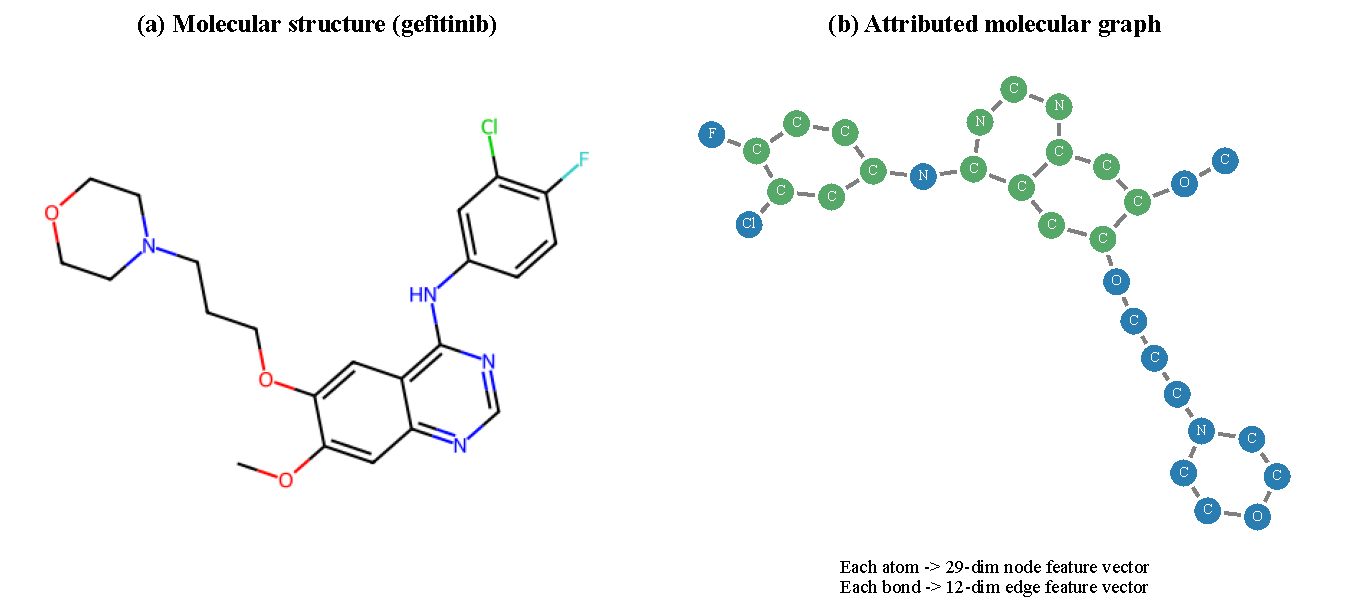
\includegraphics[width=0.95\textwidth]{molecule_to_graph.pdf}
\caption{A molecule (the EGFR inhibitor gefitinib) represented as an attributed graph of atom nodes and bond edges.}
\label{fig:intro_mol2graph}
\end{figure}

This approach offers several advantages over traditional fingerprint-based molecular
representations. First, GNNs learn task-specific molecular representations
\textit{end-to-end} from bioactivity data, rather than relying on pre-defined
structural patterns encoded in fingerprints. Second, by incorporating edge feature
vectors, GNNs can natively encode bond-level information (bond order, conjugation,
stereochemistry) that is either discarded or only coarsely approximated in
circular fingerprints. Third, deep GNN architectures can capture long-range
atomic interactions spanning multiple bonds, enabling them to model higher-order
pharmacophoric relationships that influence molecular activity \parencite{jiang2021gnn}.

Despite these advantages, the translation of GNNs from academic benchmarks to
practical drug discovery applications faces challenges, including the need for
rigorous evaluation protocols, chemical interpretability, and extension to
prospective screening pipelines---all of which are directly addressed by this thesis.

\subsection{Nepali Medicinal Plants as a Natural-Product Resource}

Nepal's Himalayan biodiversity spans roughly 6,500 flowering plant species, of which
more than 700 have documented ethnopharmacological use in Ayurvedic and Tibetan
medicine. Many are inexpensive, culturally familiar, and locally accessible, making
them an attractive yet under-explored source of natural-product leads for
resource-limited settings. The prospective screening dataset used in this thesis is
drawn from \textbf{seven traditional Nepali medicinal plant species}---\textit{Swertia
chirayita}, \textit{Rhododendron arboreum}, \textit{Nardostachys jatamansi},
\textit{Terminalia chebula}, \textit{Berberis aristata}, \textit{Ocimum sanctum}, and
\textit{Tinospora cordifolia}---selected for their documented anti-inflammatory and
antiproliferative use and their coverage in the \textbf{COCONUT~2.0} open
natural-product database \parencite{sorokina2021coconut}. After RDKit standardisation
this yields a library of \textbf{535 unique natural-product compounds} (ranging from 9
compounds for \textit{Ocimum sanctum} to 203 for \textit{Nardostachys jatamansi}) that
is screened for EGFR inhibitor activity in Chapter~4. Screening this locally accessible
chemical space directly connects computational drug discovery to Nepal's biodiversity
and offers an affordable route to candidate anti-NSCLC compounds.

% ----------------------------------------------------------------
\section{Problem Statement}
% ----------------------------------------------------------------

Despite the transformative impact of EGFR-targeted therapy and the promise of
Graph Neural Networks for drug discovery, critical and interrelated gaps persist
in both clinical practice and computational methodology.

\subsection{Clinical and Translational Need}

Acquired resistance to EGFR tyrosine kinase inhibitors---most notably the
\textbf{C797S mutation}, which renders third-generation covalent inhibitors
ineffective and for which no fourth-generation drug is yet approved---sustains a
continuing need to discover structurally novel, non-covalent EGFR inhibitor
chemotypes \parencite{rotow2023egfr}. This need is most acute in South and East Asia,
where EGFR-mutant NSCLC is highly prevalent yet novel targeted therapies remain
expensive and computational drug-discovery infrastructure is scarce. There is
therefore a clear demand for open-source, CPU-executable screening pipelines that can
prioritise affordable, regionally accessible natural-product leads---the translational
problem this thesis addresses.

\subsection{Computational Problem: Methodological Gaps in GNN-Based EGFR Inhibitor Prediction}

A review of the existing computational literature reveals three specific methodological
deficiencies that this thesis is designed to address:

\begin{enumerate}
    \item \textbf{Evaluation bias from random splitting.} The majority of published
    GNN models for molecular property prediction, including those applied to EGFR
    inhibitor classification, employ random train/test splitting. This approach allows
    structurally similar or near-identical molecular scaffolds to appear simultaneously
    in the training and test sets. As a result, the reported performance metrics
    substantially overestimate a model's ability to generalise to genuinely novel
    chemical matter---precisely the task required in prospective virtual screening.
    A model that has ``memorised'' a scaffold from the training set cannot be trusted
    to correctly classify a structurally unprecedented compound in a real screening
    campaign.

    \item \textbf{Limited molecular featurisation.} Many published GNN models for
    EGFR or related kinase targets use minimal node feature sets (e.g., atomic number
    only, or a small set of atom type flags) and ignore edge (bond) features entirely.
    This discards potentially discriminative chemical information including bond order,
    conjugation, aromaticity, and stereochemistry---all of which influence molecular
    recognition in the EGFR binding pocket.

    \item \textbf{Absence of prospective virtual screening on natural product libraries.}
    Most academic GNN studies in the EGFR domain report classification performance on
    held-out test sets but do not extend their trained models to the most practically
    relevant application: scoring and ranking an external library of unseen compounds
    to identify novel lead candidates---especially compounds derived from traditional
    medicinal plants that may offer affordable, regionally accessible therapeutic options
    \parencite{malik2025deepegfr}.
\end{enumerate}

\noindent This thesis addresses these gaps through its two objectives. First, it
\emph{builds graph neural network classifiers}---with rich 29-dimensional atom and
12-dimensional bond featurisation, evaluated under a strict Bemis-Murcko scaffold
split---and \emph{benchmarks them against traditional machine-learning baselines}
(Random Forest and an MLP on ECFP4 fingerprints), directly testing whether the added
complexity of GNNs is justified over simpler, well-established models (gaps~1--2).
Second, it \emph{deploys the best-performing models to screen} a Nepali medicinal-plant
compound library for drug-like EGFR inhibitor leads (gap~3). Because large-scale
triple-mutant bioactivity data are not yet available, the models are trained on
aggregate EGFR data, and the natural-product scaffolds they surface are intended as
candidate starting points for future experimental validation rather than as validated
triple-mutant inhibitors.

% ----------------------------------------------------------------
\section{Objectives}
% ----------------------------------------------------------------

\subsection{General Objective}

To build and benchmark a Graph Neural Network framework for EGFR inhibitor
classification against traditional machine-learning baselines, and to deploy the
best-performing models for prospective virtual screening of Nepali medicinal plant
compounds as candidate anti-NSCLC leads.

\subsection{Specific Objectives}

\begin{enumerate}
    \item To build graph neural network models that classify EGFR inhibitors and
          compare them with traditional machine-learning models.

    \item To use the best models to screen Nepali medicinal plant compounds and
          identify drug-like EGFR inhibitor leads.
\end{enumerate}

% ----------------------------------------------------------------
\section{Rationale}
% ----------------------------------------------------------------

\textbf{Clinical rationale.}
Acquired resistance to EGFR TKIs---and ultimately the triple-mutant EGFR that follows
osimertinib failure---continues to drive the search for structurally novel inhibitor
chemotypes, yet bringing new therapies through conventional drug discovery takes years
to decades. Computational virtual screening can accelerate the early stage of this
search by pre-selecting the most promising candidates for experimental testing,
reducing the number of compounds that must be synthesised and assayed. In Nepal and
South Asia, where EGFR mutations are prevalent yet targeted therapies remain expensive,
this further motivates screening locally accessible, low-cost natural-product chemical
space rather than costly synthetic libraries \parencite{rotow2023egfr}.

\textbf{Scientific rationale.}
Graph Neural Networks have demonstrated strong performance across molecular
machine learning benchmarks \parencite{hu2020strategies}, yet their application
to EGFR inhibitor discovery has been constrained by the three methodological
shortcomings enumerated in Section~1.2. Addressing all three simultaneously within a
single, reproducible pipeline---scaffold splitting, rich featurisation, systematic
multi-architecture comparison, and prospective Nepali plant compound screening---is
what motivates the design of this study.

\textbf{Data science rationale.}
This project integrates multiple core data science competencies within a single
applied research context: large-scale database querying and API integration (ChEMBL),
cheminformatics feature engineering (RDKit), deep learning architecture design and
training (PyTorch, PyTorch Geometric), automated hyperparameter search (Optuna),
prospective natural compound screening (COCONUT 2.0), and scientific visualisation
(Matplotlib, Seaborn, RDKit 2D depictions). The project therefore constitutes a comprehensive demonstration
of advanced data science methodology applied to a high-impact biomedical problem.

\textbf{Practical rationale.}
The pipeline was deliberately built from exclusively open-source Python libraries
(RDKit, PyTorch Geometric, Optuna, scikit-learn) and public databases (ChEMBL,
COCONUT~2.0), running on commodity CPU hardware, so that every reported result can be
reproduced without licensed software or specialised computing resources.

% ----------------------------------------------------------------
\section{Research Hypotheses}
% ----------------------------------------------------------------

The following two testable research hypotheses were formulated prior to
experimentation and are evaluated against the results presented in Chapter 4. Each is
stated as a null hypothesis ($H_0$) and an alternative hypothesis ($H_1$).

\begin{enumerate}
    \item \textbf{$H_1$ (Performance Hypothesis).}
    \begin{itemize}
        \item $H_0$: the best graph neural network does \emph{not} achieve a higher
        scaffold test-set AUROC than the best fingerprint baseline (Random Forest or MLP).
        \item $H_1$: the best graph neural network achieves a higher scaffold test-set
        AUROC than the best fingerprint baseline.
    \end{itemize}

    \item \textbf{$H_2$ (Virtual Screening Hypothesis).}
    \begin{itemize}
        \item $H_0$: no genuinely unseen, Lipinski-compliant Nepali plant compound is
        predicted active (predicted probability $\hat{p} \geq 0.80$ and QED $\geq 0.40$)
        by \emph{both} best models.
        \item $H_1$: at least one genuinely unseen, Lipinski-compliant Nepali plant
        compound is predicted active ($\hat{p} \geq 0.80$ and QED $\geq 0.40$) by
        \emph{both} best models, providing a candidate lead for affordable NSCLC therapy.
    \end{itemize}
\end{enumerate}

% ----------------------------------------------------------------
\section{Significance of the Study}
% ----------------------------------------------------------------

This research makes several original and complementary contributions to the
intersection of computational data science and molecular drug discovery:

\textbf{Methodological contribution.} Although systematic comparisons of GNN
architectures on molecular benchmarks are well established
\parencite{jiang2021gnn}, this thesis applies such a comparison, to the author's knowledge for
the first time, \emph{specifically to EGFR inhibitor classification}: it evaluates
five GNN architectures (GCN, GAT, GIN, AttentiveFP, GraphSAGE) against traditional
fingerprint baselines (Random Forest and MLP) under a rigorous Bemis-Murcko scaffold
split, using a rich 29-dimensional atom and 12-dimensional bond featurisation and
Bayesian hyperparameter optimisation (Optuna) for reproducible model selection. The
methodological novelty lies in this EGFR-specific, scaffold-aware, baseline-anchored
evaluation---coupled directly to the prospective natural-product screen below---rather
than in the architecture comparison in isolation.

\textbf{Natural product screening contribution.} By curating bioactive compounds
from seven traditional Nepali medicinal plant species (COCONUT 2.0) and applying the
study's best-performing models (the best graph network and the best overall
classifier) for prospective EGFR inhibition prediction, this thesis delivers the
first computational evaluation of Nepali natural products as potential EGFR TKI
candidates---directly relevant to the South Asian oncology community where EGFR
mutations are prevalent and novel therapies remain expensive.

\textbf{Translational contribution.} By extending the best-performing models into a
complete multi-model prospective virtual screening pipeline applied to
Nepali medicinal plant compounds and generating a ranked list of
Lipinski-compliant natural-product-derived
lead candidates with computed ADMET-proxy properties, the thesis delivers a concrete,
actionable output---a prioritised shortlist of natural compounds for future
experimental validation---rather than a purely academic performance comparison.

\textbf{Regional and social contribution.} The elevated prevalence of EGFR-activating
mutations in East and South Asian NSCLC patients, combined with the rising cancer
burden and limited access to novel therapies in Nepal, makes this research
particularly relevant to the South Asian academic and clinical community. The
entirely open-source, CPU-executable implementation ensures that the methodology
can be adopted and extended by researchers in resource-limited settings without
access to expensive commercial software or high-performance computing clusters.

% ----------------------------------------------------------------
\section{Limitations}
% ----------------------------------------------------------------

The following limitations of the current study are acknowledged and should be
considered when interpreting the results:

\begin{itemize}
    \item \textbf{No experimental validation.} All compound classifications and
    virtual screening predictions are purely computational. No \textit{in vitro}
    biochemical assay, cell-based proliferation assay, or \textit{in vivo}
    pharmacological experiment was conducted within the scope of this thesis.
    The predicted lead compounds remain computational hypotheses requiring
    experimental confirmation before any biological conclusions can be drawn.

    \item \textbf{Bioassay data heterogeneity.} Bioactivity data sourced from
    ChEMBL aggregates IC$_{50}$ measurements originating from hundreds of
    independent laboratories employing diverse assay formats, cell lines, and
    experimental conditions. This inherent variability introduces label noise into
    the training dataset. While pIC$_{50}$ averaging and strict data filtering
    mitigate this to some extent, residual heterogeneity may impose a ceiling on
    achievable test-set performance under scaffold splitting.

    \item \textbf{Wild-type EGFR specificity.} No dedicated, large-scale bioactivity
    dataset exists for triple-mutant EGFR (Ex19del/T790M/C797S) in ChEMBL.
    Consequently, the model was trained on the aggregate EGFR bioactivity data of
    CHEMBL203, which is dominated by wild-type and single-mutant measurements. While
    the prospective screening of structurally novel Nepali plant scaffolds is designed
    to surface chemotypes distinct from existing covalent inhibitors, the model cannot
    explicitly predict activity against the C797S mutant form.

    \item \textbf{Incomplete database coverage of Nepali medicinal flora.} The
    virtual screening library is limited to compounds recorded for the seven target
    species in the COCONUT~2.0 database. Coverage is uneven across species and many
    traditional Nepali plant compounds remain uncharacterised and absent from public
    cheminformatics databases, so the screened library is not exhaustive of the
    phytochemical diversity of these plants.

    \item \textbf{Model-sensitivity of the virtual screen.} The classifiers were
    trained on synthetic kinase inhibitors but applied to structurally dissimilar
    natural products, and the resulting hit list depends strongly on the model. As
    reported in Chapter~4, the number of predicted actives and the identity of the top
    leads differ markedly between the tuned AttentiveFP, the best graph network (GCN),
    and the best classifier (Random Forest). No single model can be treated as
    authoritative; the study mitigates this by deploying the two best models and
    prioritising cross-model consensus leads, but only experimental assay can resolve
    the residual uncertainty.

    \item \textbf{Out-of-distribution prediction reliability.} On chemical space far
    from the training distribution, the weakest model (AttentiveFP) assigned
    near-saturated probabilities to large polyphenolic tannins that fail drug-likeness
    filters, and even the best models still ranked some large, non-drug-like
    polyphenols and triterpenoids highly---indicating that such predictions must be
    interpreted with caution and coupled with physicochemical filtering.

    \item \textbf{Two-dimensional molecular representation.} The molecular graph
    encodes the constitutional (2D) topology of the molecule: atom identity and
    bonding connectivity. Three-dimensional conformational effects, induced-fit
    protein-ligand binding geometry, explicit solvent interactions, and
    protein-mediated allosteric effects are not represented in the input features.

    \item \textbf{Binary classification scope.} The study frames EGFR inhibition
    as a binary classification problem. This formulation discards the continuous
    nature of the pIC$_{50}$ scale and cannot distinguish between a moderately
    potent compound ($\text{pIC}_{50} = 6.1$) and a highly potent compound
    ($\text{pIC}_{50} = 9.5$). Continuous regression modelling of pIC$_{50}$
    values is beyond the current scope but is recommended for future work.

    \item \textbf{ADMET-proxy limitations.} The ADMET profiling in this study
    relies solely on RDKit-computed physicochemical descriptors (MW, LogP, HBD,
    HBA, TPSA, QED) as proxies for oral bioavailability. These filters do not
    capture metabolic stability, cytochrome P450 inhibition, plasma protein binding,
    blood-brain barrier permeability, hERG channel toxicity, or other critical
    ADMET parameters that determine clinical development success.
\end{itemize}

% ----------------------------------------------------------------
\section{Organisation of the Thesis}
% ----------------------------------------------------------------

The remainder of this thesis is organised as follows. \textbf{Chapter 2}
provides a comprehensive review of the relevant literature, covering the biology
of EGFR and NSCLC, the clinical development and resistance mechanisms of EGFR
TKIs, public bioactivity databases, molecular representation methods, GNN
architectures for drug discovery, traditional Nepali medicinal plants as a source
of EGFR inhibitor candidates, and virtual screening approaches. \textbf{Chapter 3} describes the complete materials and methods of the
five-phase computational pipeline, including data acquisition, molecular graph
construction, model architectures, training protocol, hyperparameter optimisation,
and the Nepali medicinal plant virtual screening workflow. \textbf{Chapter 4}
presents all experimental results with tables and analytical interpretation,
covering dataset characterisation, model benchmarking, hyperparameter tuning
outcomes, and Nepali plant virtual screening lead prioritisation.
\textbf{Chapter 5} draws the principal conclusions of the thesis and recommends
directions for future experimental and computational work.
% ================================================================
%  CHAPTER 2: LITERATURE REVIEW
% ================================================================
\chapter{Literature Review}
\label{chap:lit_review}

This chapter provides a comprehensive review of the scientific literature
underpinning this thesis. Section~\ref{sec:egfr_bio} reviews the molecular
biology of EGFR and its role in NSCLC oncogenesis. Section~\ref{sec:tki_gen}
discusses the three generations of EGFR TKIs and their clinical limitations.
Section~\ref{sec:chembl_db} describes the ChEMBL bioactivity database and
associated data quality challenges. Section~\ref{sec:molrep} reviews molecular
representation methods for machine learning. Section~\ref{sec:gnn_arch} surveys the GNN architectures employed in this study.
Section~\ref{sec:nepali_plants} reviews the Nepali medicinal plants and natural
product databases used for virtual screening.
Section~\ref{sec:vs_lit} reviews virtual screening methodologies.
Section~\ref{sec:research_gap} synthesises the identified research gaps
that motivate this thesis.

% ----------------------------------------------------------------
\section{EGFR Kinase Biology and NSCLC}
\label{sec:egfr_bio}
% ----------------------------------------------------------------

\subsection{Molecular Architecture of EGFR}

The Epidermal Growth Factor Receptor (EGFR), also designated ErbB1 or HER1,
is a 134 kDa single-pass transmembrane receptor tyrosine kinase (RTK) encoded
by the \textit{EGFR} gene on chromosome 7p11.2. EGFR is the founding member of
the ErbB receptor family (ErbB1--ErbB4), which collectively orchestrates
fundamental cellular processes including proliferation, differentiation, survival,
and motility \parencite{hynes2005erbb}. Structurally, EGFR comprises a glycosylated \textbf{extracellular domain} (I--IV)
that binds EGF-family ligands and mediates dimerisation, a single-pass
\textbf{transmembrane} helix, a regulatory \textbf{juxtamembrane} segment, and a
bilobed intracellular \textbf{kinase domain}. The ATP-binding cleft---formed at the
N-/C-lobe interface and lined by the hinge, P-loop, activation loop, and DFG
motif---is the target of all small-molecule EGFR inhibitors, and a carboxy-terminal
tail bears the autophosphorylation sites (Tyr1068, Tyr1173, and others) that recruit
downstream effectors.

Under normal conditions EGFR is autoinhibited; ligand binding drives homo- or
heterodimerisation with other ErbB members (HER2--HER4), relieving autoinhibition and
triggering \textit{trans}-autophosphorylation that activates the RAS--RAF--MEK--ERK
(MAPK), PI3K--AKT--mTOR, STAT3/5, and PLC-$\gamma$ signalling cascades---collectively
driving proliferation, survival, and differentiation \parencite{siegel2023cancer}.

\subsection{Oncogenic EGFR Mutations in NSCLC}

In non-small cell lung cancer (NSCLC), somatic gain-of-function mutations within
the EGFR kinase domain render the receptor constitutively active in a
ligand-independent manner, producing continuous, dysregulated stimulation of the
pro-survival and proliferative pathways described above \parencite{rotow2023egfr}.
This oncogenic signalling drives uncontrolled tumour growth, resistance to
apoptosis, angiogenesis, and metastatic dissemination.

The two most clinically prevalent sensitising EGFR mutations, which together
account for 85--90\% of all EGFR-mutant NSCLC, are:

\begin{itemize}
    \item \textbf{Exon 19 deletions (Ex19del)}: A heterogeneous group of in-frame
    deletions of 9--24 base pairs within exon 19, most commonly removing the
    LREA motif (residues 747--750) from the $\alpha$C-helix of the kinase N-lobe.
    These deletions stabilise the active conformation of the kinase domain by
    repositioning the $\alpha$C-helix, reducing the activation energy for catalysis.
    Ex19del accounts for approximately 45--50\% of EGFR-mutant NSCLC.
    \item \textbf{L858R point mutation}: A leucine-to-arginine substitution at
    position 858 within the activation loop (A-loop) of the kinase domain.
    This mutation disrupts the autoinhibitory network involving Leu858, Asp855,
    and Phe856 of the DFG motif, shifting the equilibrium from the inactive to
    the active kinase conformation. L858R accounts for approximately 40\% of
    EGFR-mutant NSCLC.
\end{itemize}

Rare sensitising mutations ($<$5\% combined) include exon 18 G719X, exon 20
S768I, and exon 21 L861Q. These display differential sensitivity to approved
TKIs and often require alternative treatment strategies.

The prevalence of EGFR mutations in NSCLC exhibits a profound ethnic disparity.
In Caucasian populations, EGFR mutations are found in approximately 10--15\% of
NSCLC cases, whereas in East Asian populations (Chinese, Japanese, Korean, and
related groups), the prevalence reaches 40--50\% \parencite{leonetti2019resistance}.
This epidemiological pattern reflects underlying differences in the frequency of
germline polymorphisms at the \textit{EGFR} locus that predispose to somatic
mutation acquisition. Importantly, this disparity has direct clinical relevance
for South and East Asia, including Nepal, where EGFR-targeted therapy represents
the most impactful precision oncology intervention available, yet access to
diagnostic testing and novel therapeutic agents remains significantly constrained.

% ----------------------------------------------------------------
\section{Three Generations of EGFR TKIs and Resistance Mechanisms}
\label{sec:tki_gen}
% ----------------------------------------------------------------

\subsection{First-Generation Reversible TKIs}

The clinical development of EGFR tyrosine kinase inhibitors began with the
regulatory approval of gefitinib (Iressa, AstraZeneca) in 2003 and erlotinib
(Tarceva, Genentech/Roche) in 2004. Both agents are reversible, ATP-competitive
small molecule inhibitors that occupy the EGFR ATP-binding cleft through a
combination of a hinge-region hydrogen bond (to the backbone amide nitrogen of
Met793), hydrophobic contacts with the ribose pocket, and van der Waals interactions
with the hydrophobic regions I and II of the binding site. Crystal structures of
EGFR bound to gefitinib (PDB: 2ITY) and erlotinib (PDB: 1M17) have confirmed
these binding modes at the atomic level \parencite{stamos2002egfr}.

Landmark clinical trials established the superiority of first-generation TKIs
over platinum-doublet chemotherapy in patients with sensitising EGFR mutations.
The IPASS trial (gefitinib vs. carboplatin/paclitaxel) and EURTAC trial
(erlotinib vs. platinum doublet) demonstrated objective response rates of
55--75\% and median progression-free survival (PFS) of 9--13 months---unprecedented
outcomes for a molecularly unselected metastatic NSCLC population.

However, acquired resistance develops in virtually all patients within 9--13 months.
The most common resistance mechanism (50--60\% of cases) is the \textbf{T790M
gatekeeper mutation} (Thr790Met) in exon 20 of the EGFR kinase domain
\parencite{leonetti2019resistance}. This methionine substitution acts through
two complementary mechanisms: (i) steric clash with the quinazoline scaffold
of first-generation inhibitors due to the bulkier methionine side chain, and
(ii) a 100-fold increase in the binding affinity of the kinase for ATP, effectively
out-competing the reversible TKI. Additional resistance mechanisms include MET
amplification ($\sim$5--15\%), HER2 amplification ($\sim$5--10\%), PIK3CA
mutation ($\sim$5\%), and histological transformation to small cell carcinoma
($\sim$5\%) \parencite{leonetti2019resistance}.

\subsection{Second-Generation Irreversible TKIs}

The T790M-mediated resistance to first-generation TKIs motivated the development
of second-generation irreversible inhibitors: afatinib (Gilotrif, Boehringer
Ingelheim) and dacomitinib (Vizimpro, Pfizer). These agents form a covalent
Michael addition bond with the thiol group of Cys797 at the rim of the ATP-binding
cleft, providing kinetically stable, irreversible target engagement. As pan-ErbB
inhibitors, they also inhibit HER2 and HER4 kinase activity.

Afatinib demonstrated superiority over platinum-doublet chemotherapy in the LUX-Lung
3 and LUX-Lung 6 trials, and superior PFS versus gefitinib in LUX-Lung 7, establishing
it as a first-line option for EGFR-mutant NSCLC. Dacomitinib similarly improved
PFS over gefitinib in the ARCHER 1050 trial. However, the irreversible
pan-ErbB inhibition profile of second-generation agents produces significant
dose-limiting on-target toxicity---primarily grade 3/4 diarrhoea, skin rash,
stomatitis, and paronychia---arising from inhibition of wild-type EGFR in the
gastrointestinal epithelium and skin \parencite{leonetti2019resistance}.
This toxicity profile restricts clinical dosing to sub-therapeutic levels that
are insufficient to overcome T790M-driven resistance in the majority of patients.

\subsection{Third-Generation Covalent TKIs and the C797S Resistance Problem}

The clinical unmet need created by T790M resistance drove the development of
third-generation mutant-selective covalent TKIs, led by osimertinib (Tagrisso,
AstraZeneca; AZD9291). Osimertinib was rationally designed through structure-based
drug design to selectively engage T790M-mutant EGFR while sparing wild-type EGFR.
Its indole-based acrylamide scaffold binds the EGFR ATP cleft and forms an
irreversible covalent bond with Cys797 through a Michael addition, while its
selectivity for mutant over wild-type EGFR is achieved through differential
binding geometries and kinetics rather than steric exclusion
\parencite{rotow2023egfr}.

The AURA3 trial established osimertinib as the standard second-line therapy for
T790M-positive NSCLC after first-generation TKI failure. Subsequently, the
FLAURA trial demonstrated osimertinib's superiority over first-generation TKIs
as first-line therapy (median PFS 18.9 vs. 10.2 months; overall survival 38.6
vs. 31.8 months), establishing it as the unambiguous standard of care for
EGFR-mutant NSCLC regardless of prior treatment. Additional advantages include
excellent CNS penetration ($\sim$75\% brain metastasis response rate) and an
improved safety profile compared to afatinib.

Despite these remarkable clinical achievements, acquired resistance to osimertinib
emerges in virtually all patients within 9--18 months \parencite{leonetti2019resistance}.
The dominant resistance mechanism is the \textbf{C797S mutation} (Cys797Ser),
which substitutes the cysteine residue required for covalent TKI binding with a
serine, abolishing the Michael addition reaction. C797S is detected in 20--40\%
of post-osimertinib biopsies and is of particular clinical importance when it
occurs in \textit{cis} with T790M on the same allele, generating the
\textbf{triple-mutant EGFR} (Ex19del/T790M/C797S and L858R/T790M/C797S) that is
resistant to \textit{all three generations} of approved EGFR TKIs:
\begin{itemize}
    \item First-generation TKIs cannot overcome T790M.
    \item Second-generation TKIs cannot overcome T790M steric clash at therapeutic doses.
    \item Third-generation TKIs cannot bind due to loss of the Cys797 covalent anchor.
\end{itemize}

Additional post-osimertinib resistance mechanisms include acquired MET amplification
($\sim$15\%), HER2 amplification ($\sim$5\%), RAS/RAF/MAP2K mutations ($\sim$10\%),
EGFR amplification, EGFR C797 allosteric mutations (e.g., G796S, L792 mutations),
and histological transformation to SCLC or squamous cell carcinoma
\parencite{rotow2023egfr}. As of 2026, no approved therapeutic agent effectively
addresses triple-mutant EGFR. Investigational fourth-generation strategies---including
reversible, mutant-selective non-covalent inhibitors (e.g., BLU-945) and allosteric
inhibitors that bind outside the ATP pocket (e.g., EAI045)---are in preclinical and
early clinical development, but none is yet approved and the durability of response
remains uncertain. This makes the discovery of structurally novel, non-covalent EGFR
inhibitor chemotypes---including those derived from natural products---the highest
clinical priority in NSCLC drug development.

% ----------------------------------------------------------------
\section{Bioactivity Databases and the ChEMBL Database}
\label{sec:chembl_db}
% ----------------------------------------------------------------

\subsection{Overview of the ChEMBL Database}

The ChEMBL database, maintained by EMBL-EBI, is the largest curated public repository
of bioactive small molecules and their quantitative activities
\parencite{mendez2019chembl}, comprising over 2.3 million compounds and 20 million
bioactivity measurements across more than 14,000 targets, curated primarily from the
medicinal-chemistry literature. The EGFR entry (target ID: CHEMBL203) is among its
most extensively annotated targets, reflecting decades of drug-discovery activity
around this oncology target.

\subsection{Bioactivity Endpoints and \texorpdfstring{pIC$_{50}$}{pIC50} Conversion}

The primary bioactivity endpoint used in this study is the \textbf{half-maximal
inhibitory concentration} (IC$_{50}$), defined as the concentration of a compound
required to inhibit the target activity by 50\% under specified assay conditions.
IC$_{50}$ values are expressed in molar concentration units (typically nanomolar,
nM) and span many orders of magnitude across structurally diverse compounds.

For machine learning purposes, IC$_{50}$ values are routinely converted to the
logarithmic \textbf{pIC$_{50}$} scale by taking the negative base-ten logarithm of
the molar concentration, so that higher pIC$_{50}$ values correspond to more potent
compounds. This transformation compresses the large dynamic range of IC$_{50}$
values (spanning 6--8 orders of magnitude) into a more tractable numerical range
(approximately 4--11 for drug-like compounds), improves the normality of the
activity distribution, and is the standard practice in QSAR modelling.
A threshold of pIC$_{50} \geq 6.0$ (corresponding to an IC$_{50}$ of $\leq 1\,\mu$M)
is the conventional medicinal chemistry criterion for classifying a compound as a
``hit'' or ``active'' in kinase inhibitor discovery \parencite{wu2018moleculenet}.

\subsection{Data Quality Challenges}

Utilising ChEMBL data for machine learning presents several important quality
challenges that must be addressed during data curation \parencite{wu2018moleculenet}:

\begin{itemize}
    \item \textbf{Assay heterogeneity}: IC$_{50}$ values from hundreds of laboratories
    use different assay formats and conditions, which can shift absolute values by
    1--2 orders of magnitude and add label noise.
    \item \textbf{Censored measurements}: Many values are censored ($>$ or $<$);
    standard practice retains only exact (``='') measurements.
    \item \textbf{Replicate measurements}: Repeated tests of the same compound are
    aggregated by the median pIC$_{50}$ to limit outlier influence.
    \item \textbf{Structural redundancy}: Salt forms and notation differences are
    resolved by RDKit canonicalisation and largest-fragment salt stripping.
    \item \textbf{Activity cliffs}: Structurally similar compounds with very different
    activities challenge both fingerprint- and graph-based models.
\end{itemize}

% ----------------------------------------------------------------
\section{Molecular Representation for Machine Learning}
\label{sec:molrep}
% ----------------------------------------------------------------

\subsection{Hand-Crafted Fingerprint Descriptors}

Molecular fingerprints are fixed-length binary or integer vectors that encode
the presence or count of predefined structural features within a molecule.
They represent the dominant molecular representation paradigm in traditional
cheminformatics and remain strong baselines for bioactivity prediction tasks.

\subsubsection{Extended Connectivity Fingerprints (ECFP)}

The Extended Connectivity Fingerprint (ECFP) \parencite{rogers2010ecfp}, also
known as the Morgan fingerprint (after its algorithmic basis in the Morgan
algorithm for canonical atom numbering), is the most widely used molecular
fingerprint in cheminformatics. ECFP encodes circular atomic neighbourhoods
through an iterative procedure:

\begin{enumerate}
    \item Each atom is assigned an initial integer identifier based on six atomic
    invariants (atomic number, degree, number of hydrogens, charge, isotope,
    and ring membership).
    \item At each iteration $r$ (radius), each atom's identifier is updated by
    hashing together its current identifier with the identifiers of its immediate
    neighbours (corresponding to atoms within $r$ bonds).
    \item All identifiers generated at each iteration up to radius $r$ are
    collected and folded into a bit vector of specified length (typically 1024
    or 2048 bits) using a hash function.
\end{enumerate}

ECFP4 (radius = 2, 2048 bits) is the de facto standard, encoding circular
substructures up to 4 bonds in diameter. Its advantages include computational
efficiency ($O(N)$ in molecular size), interpretability of individual bits as
specific substructural features, and strong empirical performance across diverse
QSAR benchmarks. Limitations include: (i) fixed-length encoding discards
variable-size topological patterns not captured within the predefined radius;
(ii) bit collisions in folded fingerprints reduce information content;
(iii) bond-level information (bond type, conjugation, stereochemistry) is only
coarsely encoded; and (iv) the representation is not differentiable, precluding
end-to-end learning of task-optimal molecular representations.

\subsubsection{Other Descriptor Types}

Beyond fingerprints, molecular property prediction has traditionally relied on
physicochemical descriptors (e.g., RDKit 2D and 3D descriptors, MACCS keys,
DRAGON descriptors), shape-based 3D pharmacophore fingerprints, and continuous
molecular embeddings derived from SMILES string language models.

For the purposes of this study, ECFP4 fingerprints are used for both traditional
machine learning baselines. \textbf{Random Forest (RF)} is an ensemble of 500
decision trees with balanced class weighting and \texttt{max\_features='sqrt'},
providing a well-calibrated, sample-efficient baseline for medium-sized bioactivity
datasets. The \textbf{Multi-Layer Perceptron (MLP)} baseline is a three-layer
neural network (2048$\to$512$\to$128$\to$1) operating on the same ECFP4 inputs,
trained with BCEWithLogitsLoss and early stopping. The MLP bridges the gap between
fingerprint-based and graph-based deep learning, allowing direct attribution of
performance differences to the graph representation rather than to deep learning
capacity in general.

\subsection{Graph-Based Molecular Representations}

The fundamental insight motivating the graph-based approach is that a molecule
is inherently a labelled graph: atoms are nodes with associated chemical properties,
and bonds are edges with associated chemical characteristics. This isomorphism
allows molecules to be fed directly into graph processing algorithms without
information-losing pre-encoding steps \parencite{gilmer2017neural}.

A molecular graph is defined by three components:
\begin{itemize}
    \item A set of \textbf{nodes}, where each node represents one heavy atom and
    carries a node feature vector describing that atom's chemical properties.
    \item A set of \textbf{edges}, where each edge represents one chemical bond and
    carries an edge feature vector describing that bond's properties.
    \item The \textbf{bonding connectivity}, recording which atoms are bonded to
    which.
\end{itemize}

The dimensionality and content of the node and edge feature vectors directly
determine the chemical information available to the model. In this work, a
comprehensive 29-dimensional node feature vector and 12-dimensional edge feature
vector were designed to capture the chemical information most relevant to kinase
inhibitor classification, as detailed in Chapter 3.

\subsection{Graph Neural Networks: The Message-Passing Framework}

The general message-passing neural network (MPNN) framework \parencite{gilmer2017neural}
provides a unified description of most GNN architectures. In this framework, each
atom maintains a hidden representation that is refined layer by layer through two
operations, illustrated in Figure~\ref{fig:msgpass}:

\textbf{Aggregation}: each atom collects ``messages'' from its bonded neighbours,
where each message is a learned function of the central atom's representation, the
neighbour's representation, and the connecting bond features. The messages are then
combined using a permutation-invariant operator (sum, mean, or max) so that the
result does not depend on the arbitrary ordering of neighbours.

\textbf{Update}: each atom updates its own hidden representation by combining its
previous state with the aggregated message, typically through a small multilayer
perceptron or a gated recurrent unit.

After several message-passing layers, a \textbf{readout function} aggregates all
the atom-level representations into a single graph-level embedding, which is then
passed to a task-specific head (for example, a fully connected classifier for
binary activity prediction).

\begin{figure}[htbp]
\centering
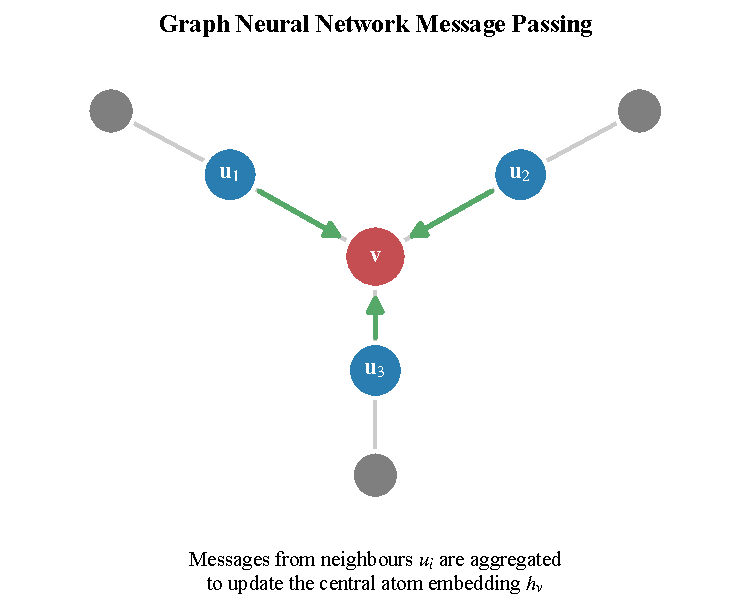
\includegraphics[width=0.62\textwidth]{gnn_message_passing.pdf}
\caption{One step of GNN message passing: atom $v$ aggregates learned messages from its bonded neighbours $u_1,u_2,u_3$.}
\label{fig:msgpass}
\end{figure}

The key advantages of the MPNN framework for molecular property prediction are:
(i) the representation is learned end-to-end from bioactivity data, requiring
no expert-designed feature engineering; (ii) arbitrary atom- and bond-level
information can be incorporated via the node and edge feature vectors; (iii) the
framework naturally handles molecules of varying size without fixed-length encoding;
and (iv) the learned representations capture both local chemical environments
(from lower layers) and global molecular topology (from higher layers through
the readout).

% ----------------------------------------------------------------
\section{Graph Neural Network Architectures for Drug Discovery}
\label{sec:gnn_arch}
% ----------------------------------------------------------------

\subsection{Graph Convolutional Network (GCN)}

The Graph Convolutional Network (GCN) \parencite{kipf2017gcn} introduced the
concept of spectral graph convolution through a computationally tractable
first-order approximation. At each layer, every atom's representation is updated by
taking a degree-normalised average of the (linearly transformed) representations of
its bonded neighbours together with its own, followed by a non-linear activation.
The normalisation uses the atom degrees (with self-loops added) so that atoms with
many bonds do not dominate the aggregation.

The GCN architecture has several notable limitations in the context of molecular
property prediction. First, the degree-normalised aggregation weights all
neighbouring atoms equally, without learning which chemical neighbours contribute
most to a given property. Second, standard GCN implementations use node features
only and do not incorporate edge features, discarding bond-level chemical
information. Third, GCN is limited in its expressive power: it cannot distinguish
certain pairs of non-isomorphic graph structures that differ only in their
higher-order topology, limiting its ability to discriminate complex pharmacophoric
patterns \parencite{xu2019gin}. Despite these limitations, GCN provides a strong
and computationally efficient baseline and demonstrated competitive AUROC
performance in the TDC ADMET benchmarks \parencite{huang2021therapeutics}.

\subsection{Graph Attention Network (GAT)}

The Graph Attention Network (GAT) \parencite{velickovic2018gat} replaces the GCN's
fixed degree-based averaging with learnable attention coefficients: each neighbour's
contribution to an atom's update is weighted by a learned score computed from the two
atoms' representations. Several parallel attention ``heads'' are used---concatenated
in intermediate layers and averaged in the final one---and the GATv2 extension
\parencite{brody2022attentive} fixes the ``static attention'' limitation of the
original formulation by conditioning the weights dynamically on both the query and key
nodes. This lets the network focus on the atoms most relevant to activity, such as the
hinge-binding nitrogens of the quinazoline pharmacophore over solvent-exposed
substituents.

\subsection{Graph Isomorphism Network (GIN)}

The Graph Isomorphism Network (GIN) \parencite{xu2019gin} was developed from
a theoretical analysis of the representational limits of GNNs within the
message-passing framework. Xu et al. proved that the expressive power of any
message-passing GNN is bounded by the Weisfeiler-Leman (WL) graph isomorphism
test, and demonstrated that GIN achieves this theoretical upper bound. The GIN
layer updates each atom by \textit{summing} its neighbours' representations, adding
the atom's own representation (scaled by a small learnable factor), and passing the
result through a multilayer perceptron.

The critical theoretical insight is that sum aggregation preserves multiset
information about neighbour features (unlike mean or max aggregation, which
can conflate distinct neighbourhood configurations), making GIN maximally
expressive among message-passing GNNs.

The GINEConv \parencite{hu2020strategies} extension incorporates edge features by
adding a transformed bond feature vector to each neighbour's representation before
the summation, so that bond-level chemistry informs the aggregation.

Despite its theoretical superiority, GIN does not always outperform architecturally
simpler GNNs on molecular property prediction benchmarks, suggesting that
the WL-level expressivity gains are primarily relevant for highly symmetric
graph structures that are uncommon in drug-like molecules. Empirically, GIN has
shown strong performance on graph classification tasks in the TU graph benchmarks
and MoleculeNet \parencite{wu2018moleculenet}.

\subsection{AttentiveFP}

AttentiveFP \parencite{xiong2020attentivefp} is a GNN purpose-built for molecular
property prediction, combining two mechanisms. At the \textbf{atom level}, attention
weights modulating each neighbour's contribution are computed from the two atoms'
representations \emph{together with the connecting bond's feature vector}, natively
integrating edge chemistry into the attention. At the \textbf{molecule level}, an
iterative readout refines a single molecular embedding: a context vector, initialised
from the mean atom representation, repeatedly attends over all atoms and is updated by
a Gated Recurrent Unit (GRU) over several timesteps, capturing progressively more
global structure. AttentiveFP reaches near state-of-the-art performance on several
MoleculeNet benchmarks \parencite{xiong2020attentivefp, jiang2021gnn}, which is why it
was chosen as the architecture for hyperparameter optimisation here---although the
benchmark in Chapter~4 ultimately found it the weakest of the five graph networks on
the scaffold test set.


\subsection{GraphSAGE}

GraphSAGE (Graph SAmple and aggreGatE) \parencite{hamilton2017graphsage} is an
inductive framework that learns aggregation functions from sampled local
neighbourhoods rather than the full adjacency matrix. Each atom forms the mean of its
neighbours' representations, concatenates this with its own previous representation,
and passes the result through a learnable transformation---preserving the atom's
identity alongside its local context. Mean aggregation is robust to high-degree atoms,
and the inductive formulation generalises naturally to novel scaffolds, which is
directly relevant under Bemis-Murcko evaluation. Here GraphSAGE uses BatchNorm and
concatenated mean+max pooling, following the same readout as GCN.

% ----------------------------------------------------------------
\section{Nepali Medicinal Plants and Natural Product Databases}
\label{sec:nepali_plants}
% ----------------------------------------------------------------

\subsection{Traditional Medicinal Plants in Nepal}

Nepal harbours remarkable biodiversity, hosting approximately 6,500 flowering plant
species within a geographic transect spanning tropical lowlands ($\sim$60 m a.s.l.)
to alpine zones ($>$5,000 m a.s.l.). Of these, over 700 species have documented
medicinal uses in traditional Ayurvedic and Tibetan medical systems.
Several Nepali medicinal plants have been
ethnopharmacologically associated with anticancer activity and are candidates
for systematic computational evaluation as potential EGFR inhibitor sources.

Seven species were selected on the basis of documented bioactivity, coverage in
COCONUT 2.0, and relevance to oncological conditions:
\begin{itemize}
    \item \textbf{\textit{Swertia chirayita}} (Chirayito) --- xanthones and secoiridoids;
    \item \textbf{\textit{Rhododendron arboreum}} (Lali Gurans) --- triterpenoids and flavonoids;
    \item \textbf{\textit{Nardostachys jatamansi}} (Jatamansi) --- sesquiterpenes;
    \item \textbf{\textit{Terminalia chebula}} (Haritaki) --- hydrolysable tannins, a Triphala constituent;
    \item \textbf{\textit{Berberis aristata}} (Chutro) --- the alkaloid berberine, with reported EGFR-pathway modulation;
    \item \textbf{\textit{Ocimum sanctum}} (Tulsi) --- eugenol and ursolic/rosmarinic acids, with reported EGFR-inhibitory activity;
    \item \textbf{\textit{Tinospora cordifolia}} (Giloy) --- diterpenoids and isoquinoline alkaloids.
\end{itemize}
All seven have ethnopharmacologically documented anti-inflammatory or antiproliferative use.

\subsection{The COCONUT 2.0 Database}

The \textbf{CO}llection of \textbf{O}pen \textbf{N}atural Prod\textbf{U}c\textbf{T}s
(COCONUT) is the largest freely available database of natural product structures,
curated and maintained by the Steinbeck group at Friedrich Schiller University Jena
\parencite{sorokina2021coconut}. COCONUT 2.0 contains over 400,000 unique natural
product structures drawn from more than 50 public natural product databases,
each associated with organism taxonomy, literature references, and precomputed
molecular descriptors. Structures are provided as canonical SMILES and InChI strings
with CAS registry numbers where available.

For this study, COCONUT 2.0 was used to retrieve SMILES for compounds annotated to
the seven Nepali plant species of interest using organism taxonomy matching. Retrieved
compounds were then subjected to the same preprocessing pipeline as the ChEMBL training
data (salt removal, SMILES canonicalisation, MW $\leq$ 1000 Da, RDKit validation) to
ensure featurisation consistency.

% ----------------------------------------------------------------
\section{Virtual Screening in Drug Discovery}
\label{sec:vs_lit}
% ----------------------------------------------------------------

\subsection{Overview of Virtual Screening}

Virtual screening (VS) is a computational strategy employed at the early stage
of drug discovery to prioritise a large library of candidate compounds for
experimental testing, based on predicted interaction with a biological target
or predicted biological activity. VS substantially reduces the number of compounds
that need to be synthesised and assayed experimentally, focusing experimental
resources on the most promising candidates \parencite{walters2020generative}.

Two principal paradigms of VS are distinguished:
\begin{itemize}
    \item \textbf{Structure-based virtual screening (SBVS)}: Requires a
    three-dimensional crystal or cryo-EM structure of the target protein. Molecular
    docking algorithms (AutoDock Vina, Glide, GOLD) predict the binding pose and
    estimate the binding affinity of each candidate compound within the target's
    binding site. SBVS is accurate but computationally intensive and requires
    high-resolution structural data.
    \item \textbf{Ligand-based virtual screening (LBVS)}: Does not require target
    structural knowledge. A model trained on known active and inactive compounds
    (e.g., from ChEMBL) is used to score and rank external compound libraries by
    predicted activity probability. LBVS is computationally scalable to millions
    of compounds and is particularly powerful when high-quality bioactivity training
    data is available.
\end{itemize}

This thesis implements a \textbf{ligand-based virtual screening} pipeline using its
two best-performing trained classifiers---the best graph neural network (GCN) and a
Random Forest baseline---as the scoring functions, and prioritising leads by
cross-model consensus rather than relying on any single model.

\subsection{GNN-Based Virtual Screening}

The landmark application of GNN-based virtual screening in drug discovery was
the discovery of \textbf{halicin} by Stokes et al. \parencite{stokes2020deep}
at the Collins Laboratory (MIT). A directed-message passing neural network (DMPNN)
was trained on 2,335 compounds from the Drug Repurposing Hub to predict broad-spectrum
antibiotic activity. The trained model was applied to score over 100 million compounds
from the ZINC15 database; halicin (SU-3327, a c-Jun N-terminal kinase inhibitor)
was identified as a top-ranked hit and subsequently validated as a potent,
broad-spectrum antibiotic in mouse models of \textit{Acinetobacter baumannii}
infection. This study demonstrated that GNN-based LBVS can identify structurally
novel bioactive compounds that escape detection by conventional similarity searches.

In the kinase inhibitor domain, GNN-based VS has been applied to several targets
including EGFR, CDK2, and VEGFR2, typically achieving hit rates of 10--50\% in
subsequent experimental validation---substantially higher than the 0.1--1\% hit
rates typical of unguided high-throughput screening \parencite{sun2021gcn}.

\subsection{Natural Product Libraries and Nepali Medicinal Plants}

A key methodological choice in virtual screening is the source and composition of
the screening library. This thesis employs a \textbf{natural product library} strategy:
bioactive compounds from seven traditional Nepali medicinal plant species are retrieved
from the COCONUT 2.0 database and used as the screening library. The biological and
ethnopharmacological rationale is well-established: plants such as
\textit{Swertia chirayita}, \textit{Berberis aristata}, and \textit{Ocimum sanctum}
have centuries of documented use in the treatment of cancer-related symptoms and have
yielded structurally diverse secondary metabolites---alkaloids, flavonoids, terpenes,
and tannins---that represent structurally distinct chemotypes compared to synthetic
kinase inhibitors, potentially offering novel scaffolds capable of engaging the EGFR
ATP-binding pocket through unconventional binding modes. This strategy directly
connects computational drug discovery to the biodiversity resources and traditional
knowledge of Nepal, supporting affordable and regionally accessible cancer therapeutic
research.

\subsection{ADMET Properties and Lead Prioritisation}

Virtual screening hit lists require secondary filtering by predicted ADMET
(Absorption, Distribution, Metabolism, Excretion, Toxicity) properties to
prioritise compounds with the greatest potential for clinical development
\parencite{walters2020generative}. In this study, ADMET-proxy properties were
computed using RDKit as physicochemical surrogates:

\begin{itemize}
    \item \textbf{Lipinski's Rule of Five (Ro5)}: MW $\leq$ 500 Da, LogP $\leq$ 5,
    HBD $\leq$ 5, HBA $\leq$ 10 as necessary (not sufficient) conditions for
    oral bioavailability \parencite{lipinski2001experimental}.
    \item \textbf{Quantitative Estimate of Drug-likeness (QED)}: A composite
    drug-likeness score (range 0--1) integrating MW, LogP, HBD, HBA, TPSA, number
    of aromatic rings, number of rotatable bonds, and the presence of structural
    alerts, calibrated to reflect the desirability profile of approved oral drugs
    \parencite{bickerton2012quantifying}.
    \item \textbf{Topological Polar Surface Area (TPSA)}: A molecular surface
    area descriptor correlated with oral absorption and blood-brain barrier
    permeability. Values $\leq$ 140 \AA$^2$ are associated with adequate
    gastrointestinal absorption.
\end{itemize}

% ----------------------------------------------------------------
\section{Research Gap}
\label{sec:research_gap}
% ----------------------------------------------------------------

A systematic analysis of the reviewed literature reveals three persistent and
interrelated methodological gaps in the application of Graph Neural Networks to
EGFR inhibitor discovery. These gaps collectively limit the clinical utility and
scientific rigour of existing computational approaches:

\begin{enumerate}
    \item \textbf{Evaluation Bias from Random Data Splitting.} The majority of
    published GNN models for EGFR or related kinase bioactivity prediction employ
    random train/test splitting \parencite{jiang2021gnn, malik2025deepegfr}.
    This practice allows molecules with near-identical Bemis-Murcko scaffolds to
    appear simultaneously in training and test partitions, creating an optimistic
    bias in reported performance metrics. A model that achieves 0.90 AUROC under
    random splitting may perform significantly worse when deployed on a genuinely
    novel scaffold---precisely the scenario encountered in prospective virtual
    screening. Scaffold-based splitting, which groups all molecules sharing the
    same core framework into a single partition, provides a more realistic and
    demanding assessment of model generalisation \parencite{wu2018moleculenet}.

    \item \textbf{Incomplete Molecular Featurisation.} Published GNN models for
    EGFR inhibitor classification frequently employ minimal node feature sets
    (e.g., atom type only, or a small number of atomic properties) and rarely
    incorporate explicit, multi-dimensional bond-level (edge) feature vectors
    \parencite{malik2025deepegfr}. Bond features encoding stereochemistry,
    conjugation, and aromaticity carry significant pharmacological information---for
    example, the aromatic bonds of the quinazoline hinge-binder scaffold and the
    acrylamide double bond of covalent inhibitors---that is discarded or only
    coarsely approximated by node-only models or ECFP fingerprints.

    \item \textbf{Lack of Prospective Screening on Natural Product and Regionally
    Relevant Compound Libraries.} Most academic GNN papers in the EGFR and kinase
    inhibitor domain report performance metrics on held-out test sets but do not
    deploy the trained model in a prospective virtual screening pipeline applied
    to natural product or ethnopharmacological compound collections
    \parencite{sun2021gcn, malik2025deepegfr}. For South Asian research communities
    where EGFR-mutant NSCLC is prevalent but novel targeted therapies are expensive
    and inaccessible, virtual screening of traditional medicinal plant compounds
    represents a high-impact translational application that is entirely absent from
    the computational EGFR inhibitor literature.
\end{enumerate}

\noindent Table~\ref{tab:gap_compare} formally positions this thesis against
representative published GNN studies for EGFR inhibitor prediction.

\begin{table}[H]
\centering
\caption{This thesis versus representative GNN-based EGFR studies across three methodological dimensions ($\checkmark$ addressed; $\circ$ partial; $\times$ absent).}
\label{tab:gap_compare}
{\singlespacing
\begin{tabular}{lccc}
\toprule
\multirow{2}{*}{\textbf{Study}} &
\textbf{Scaffold} & \textbf{Rich} & \textbf{Natural Product} \\
& \textbf{Split} & \textbf{Features} & \textbf{Screening} \\
\midrule
DeepEGFR \parencite{malik2025deepegfr}      & $\times$ & $\circ$ & $\times$ \\
GCN QSAR \parencite{jiang2021gnn}           & $\times$ & $\circ$ & $\times$ \\
AttentiveFP \parencite{xiong2020attentivefp} & $\times$ & $\checkmark$ & $\times$ \\
Hu et al. \parencite{hu2020strategies}      & $\circ$  & $\checkmark$ & $\times$ \\
\textbf{This Thesis}                        & $\checkmark$ & $\checkmark$ & $\checkmark$ \\
\bottomrule
\end{tabular}
}
\end{table}

This thesis addresses all three gaps through its two objectives, within a single
reproducible open-source pipeline. To close the evaluation and featurisation gaps
(1--2), it \textbf{benchmarks graph neural networks}---built with comprehensive
29-dimensional node and 12-dimensional edge features and tuned via Optuna---%
\textbf{against traditional machine-learning baselines} under a strict Bemis-Murcko
scaffold split. To close the screening gap (3), it \textbf{deploys the best-performing
models} in a prospective virtual screen of Nepali medicinal plant compounds from
COCONUT~2.0 with ADMET-proxy prioritisation.
\chapter{Materials and Methods}

\section{System Flow Diagram of the Computational Framework}

\subsection{Overview of the Computational Framework}

The overall methodology follows a systematic five-phase pipeline as illustrated in
Figure~\ref{fig:workflow}. All code was implemented in Python 3.14 using
exclusively open-source libraries and executed on a macOS system (CPU).

\begin{figure}[htbp]
\centering
\begin{tikzpicture}[
  node distance=0.55cm,
  phase/.style={rectangle, rounded corners=6pt, draw=black, thick,
                fill=blue!20, minimum width=7.6cm, minimum height=0.7cm,
                align=center, font=\bfseries\small},
  proc/.style={rectangle, rounded corners=4pt, draw=black,
               fill=cyan!12, minimum width=7.2cm, minimum height=0.5cm,
               align=center, font=\small},
  final/.style={rectangle, rounded corners=6pt, draw=black, very thick,
                fill=green!25, minimum width=7.6cm, minimum height=0.7cm,
                align=center, font=\bfseries\small},
  arr/.style={->, thick, >=latex}
]
\node[phase] (ph1) {Phase 1: Data Acquisition \& Preprocessing};
\node[proc, below=0.2cm of ph1] (p1a) {ChEMBL CHEMBL203 retrieval via REST API};
\node[proc, below=of p1a] (p1b) {pIC$_{50}$ conversion, binary labelling, RDKit curation};
\node[proc, below=of p1b] (p1c) {Exploratory data analysis (class balance, scaffold diversity)};
\node[phase, below=0.5cm of p1c] (ph2) {Phase 2: Molecular Graph Construction};
\node[proc, below=0.2cm of ph2] (p2a) {29-dim node features + 12-dim edge features};
\node[phase, below=0.5cm of p2a] (ph3) {Phase 3: Model Development \& Training};
\node[proc, below=0.2cm of ph3] (p3a) {\textbf{5 GNNs} (GCN, GAT, GIN, AttentiveFP, GraphSAGE)\\\textbf{vs.\ 2 traditional ML baselines} (Random Forest, MLP)};
\node[phase, below=0.5cm of p3a] (ph4) {Phase 4: Evaluation \& Benchmarking};
\node[proc, below=0.2cm of ph4] (p4a) {AUROC, AUPRC, F1, MCC on scaffold test set};
\node[phase, below=0.5cm of p4a] (ph5) {Phase 5: Nepali Plant Virtual Screening};
\node[proc, below=0.2cm of ph5] (p5a) {\textbf{Select 7 Nepali medicinal plant species}\\(documented anti-cancer / anti-inflammatory use $+$ COCONUT~2.0 coverage)};
\node[proc, below=of p5a] (p5b) {COCONUT 2.0 retrieval + RDKit standardisation $\rightarrow$ 535 compounds};
\node[proc, below=of p5b] (p5c) {Score with \textbf{best models} (GCN $+$ Random Forest consensus)\\$+$ Lipinski Ro5, QED, ADMET-proxy filtering};
\node[final, below=0.5cm of p5c] (out) {Ranked Nepali Natural-Product Lead Candidates};

\foreach \a/\b in {ph1/p1a, p1a/p1b, p1b/p1c, p1c/ph2, ph2/p2a, p2a/ph3,
                   ph3/p3a, p3a/ph4, ph4/p4a, p4a/ph5,
                   ph5/p5a, p5a/p5b, p5b/p5c, p5c/out}
  \draw[arr] (\a) -- (\b);
\end{tikzpicture}
\caption{Five-phase pipeline: benchmarking five GNNs against traditional ML baselines, then screening Nepali medicinal-plant compounds with the best models.}
\label{fig:workflow}
\end{figure}

\section{Data Acquisition}

\subsection{Target Selection}

The primary target for bioactivity data retrieval was the Epidermal Growth Factor
Receptor (EGFR), indexed in ChEMBL as target identifier \texttt{CHEMBL203}. EGFR
was selected as the model target because it is a clinically validated oncology
target in NSCLC, and CHEMBL203 aggregates the largest publicly available collection
of quantitative EGFR inhibition bioactivity measurements.

\subsection{Bioactivity Data Retrieval}

Bioactivity data was retrieved programmatically from the ChEMBL database using the
\texttt{chembl-webresource-client} Python library, which queries the then-current
ChEMBL release through the REST API (retrieved May 2026). The query was
restricted to compounds satisfying the following criteria:
\begin{itemize}
    \item \textbf{Standard type}: IC$_{50}$ (half-maximal inhibitory concentration)
    \item \textbf{Standard relation}: Exact value only (\texttt{=})
\end{itemize}

Records with missing SMILES strings, missing IC$_{50}$ values, or non-exact
relations ($>$, $<$, $\geq$, $\leq$) were excluded. IC$_{50}$ values reported
in ChEMBL for this target are in nanomolar (nM) units, as assumed throughout
the pIC$_{50}$ conversion. The raw dataset contained
approximately 19,000 compound-activity pairs prior to deduplication and cleaning.

\subsection{Data Cleaning and Labelling}

The raw IC$_{50}$ values (in nanomolar units) were converted to the logarithmic
pIC$_{50}$ scale by taking the negative base-ten logarithm of the molar
concentration, so that more potent compounds receive higher pIC$_{50}$ scores.
Binary activity labels were then assigned using the standard medicinal chemistry
threshold: compounds with a pIC$_{50}$ of at least 6.0 were labelled \textit{active},
and those below 6.0 were labelled \textit{inactive}. This threshold corresponds to
an IC$_{50}$ of $\leq 1~\mu$M. For compounds with multiple reported measurements,
the median pIC$_{50}$ was used to obtain a single robust value per molecule.

\subsection{Molecular Standardisation and Filtering}

Molecular standardisation was performed using RDKit (version 2026.3.2):
\begin{itemize}
    \item \textbf{Salt removal}: The largest fragment was retained for each compound.
    \item \textbf{Canonicalisation}: SMILES strings were canonicalised to ensure
          unique molecular representation.
    \item \textbf{Molecular weight filter}: Compounds with MW $>$ 1000 Da
          were excluded.
    \item \textbf{Deduplication}: Duplicate canonical SMILES were collapsed using
          the median pIC$_{50}$.
\end{itemize}

The final curated dataset comprised \textbf{10,523 unique compounds}, distributed
as 7,792 actives (74.0\%) and 2,731 inactives (26.0\%).

\subsection{Exploratory Data Analysis}

Prior to molecular graph construction, an exploratory data analysis (EDA) step was
performed on the cleaned dataset to characterise its statistical structure and inform
modelling decisions. Using RDKit and pandas, the analysis quantified the class
balance, the distribution of pIC$_{50}$ potency values, the ranges of the
physicochemical properties (molecular weight, LogP), and the Bemis-Murcko scaffold
diversity (number of unique scaffolds and the proportion of singleton scaffolds).
This characterisation, reported in Chapter~4, both confirms the integrity of the
curated dataset and motivates the use of scaffold-based splitting, given the
long-tailed scaffold distribution observed.

\section{Molecular Graph Construction}

\subsection{Graph Representation}

Each molecule was converted to an undirected graph using
PyTorch Geometric (version 2.7.0), where every node represents an atom and every
edge represents a chemical bond (the molecule-to-graph conversion is illustrated in
Figure~\ref{fig:intro_mol2graph}). Each atom node carries a 29-dimensional feature
vector and each bond edge a 12-dimensional feature vector, detailed below.

\subsection{Node Features}

Each atom was represented by a 29-dimensional feature vector encoding:
\begin{itemize}
    \item \textbf{Atom type} (one-hot, 10 dim): C, N, O, S, F, Cl, Br, I, P, Unknown
    \item \textbf{Atom degree} (one-hot, 6 dim): 0, 1, 2, 3, 4, $\geq$5
    \item \textbf{Formal charge} (1 dim): integer value
    \item \textbf{Hydrogen count} (one-hot, 5 dim): 0, 1, 2, 3, $\geq$4
    \item \textbf{Hybridisation} (one-hot, 5 dim): SP, SP2, SP3, SP3D, SP3D2
    \item \textbf{Aromaticity} (binary, 1 dim)
    \item \textbf{Ring membership} (binary, 1 dim)
\end{itemize}

\subsection{Edge Features}

Each bond was represented by a 12-dimensional edge feature vector encoding:
\begin{itemize}
    \item \textbf{Bond type} (one-hot, 4 dim): Single, Double, Triple, Aromatic
    \item \textbf{Conjugation} (binary, 1 dim)
    \item \textbf{Ring membership} (binary, 1 dim)
    \item \textbf{Stereochemistry} (one-hot, 6 dim): STEREONONE, STEREOANY,
          STEREOZ, STEREOE, STEREOCIS, STEREOTRANS
\end{itemize}

\section{Data Splitting}

To ensure rigorous evaluation on genuinely novel chemical scaffolds, a deterministic
\textbf{Bemis-Murcko Scaffold Split} was implemented using RDKit. The Bemis-Murcko
algorithm extracts the core macrocyclic framework of each molecule by retaining ring
systems, linker atoms, and chain atoms connected to rings while removing side chains.
Compounds sharing identical scaffold hashes were allocated exclusively to one split
partition. The dataset was partitioned as follows:

\begin{table}[H]
\centering
\caption{Dataset partitioning using the Bemis-Murcko scaffold split.}
\label{tab:split}
\begin{tabular}{lccc}
\toprule
\textbf{Partition} & \textbf{Proportion} & \textbf{Compounds} & \textbf{Unique Scaffolds} \\
\midrule
Training   & 80\% & 8,418  & majority \\
Validation & 10\% & 1,052  & held-out \\
Test       & 10\% & 1,053  & held-out \\
\bottomrule
\end{tabular}
\end{table}

\section{Machine Learning Model Development}

\subsection{Traditional Baseline Models}

Two traditional machine learning baselines were implemented using
scikit-learn (version 1.8.0) trained on 2048-bit ECFP4 (Morgan) fingerprints
(radius = 2) computed by RDKit:

\begin{itemize}
    \item \textbf{Random Forest (RF)}: An ensemble of 500 decision trees with
          \texttt{class\_weight=} \texttt{'balanced'} to account for the 74:26 class imbalance.
          Hyperparameters included \texttt{max\_features='sqrt'} and
          \texttt{min\_samples\_leaf=1}.
    \item \textbf{Multi-Layer Perceptron (MLP)}: A three-layer neural network
          (2048$\to$512$\to$128$\to$1) with BatchNorm and Dropout(0.3) at each hidden
          layer, trained on ECFP4 fingerprints with BCEWithLogitsLoss (pos\_weight),
          Adam optimiser, and early stopping (patience = 10) on an internal 90/10
          validation split. This evaluates whether deep learning on fingerprint features
          alone offers benefits beyond the Random Forest ensemble.
\end{itemize}

\subsection{Graph Neural Network Architectures}

Five GNN architectures were implemented using PyTorch Geometric. Each learns atom
embeddings by repeatedly aggregating information from bonded neighbours, pools them
into a single molecular vector, and outputs an activity probability through a final
sigmoid layer,
\begin{equation}
\hat{p} = \sigma(z) = \frac{1}{1+e^{-z}} \in (0,1).
\end{equation}
The architectures differ only in how each atom aggregates information from its
neighbours, described below.

\subsubsection{Graph Convolutional Network (GCN)}

The GCN propagates information using degree-normalised spectral convolution. At
each layer, every atom embedding is updated by averaging the transformed
embeddings of its bonded neighbours and itself, where the averaging weights are
normalised by the degrees of the participating atoms (with added self-loops). This
symmetric normalisation prevents high-degree atoms from dominating the
representation. Three convolutional layers were stacked, each followed by batch
normalisation, a ReLU non-linearity, and dropout.

\subsubsection{Graph Attention Network (GAT)}

The GAT replaces the fixed normalisation of the GCN with learnable attention
weights: for each atom, the contribution of every neighbour is weighted by an
attention coefficient computed from the two atoms' embeddings and the connecting
bond features, then normalised across all neighbours. This lets the network learn
which bonds and substructures are most relevant to activity. Four attention heads
were used in the intermediate layers (their outputs concatenated) and a single
averaged head in the final layer. Bond (edge) features were supplied directly to
the attention mechanism through the GATv2 formulation.

\subsubsection{Graph Isomorphism Network (GIN)}

GIN is the most theoretically expressive message-passing scheme within the
Weisfeiler--Lehman framework. Rather than averaging, each atom embedding is updated
by summing its neighbours' embeddings (preserving multiset information that mean or
max aggregation would discard), adding the atom's own embedding, and passing the
result through a two-layer multilayer perceptron. The GINEConv variant used here
extends this update to incorporate the 12-dimensional bond feature vectors.

\subsubsection{GraphSAGE}

GraphSAGE \parencite{hamilton2017graphsage} updates each atom by combining its own
previous embedding with the mean of its neighbours' embeddings and passing the
combination through a learnable transformation. Because the update depends only on
local neighbourhood aggregation rather than the global graph structure, GraphSAGE
is inherently inductive and generalises naturally to unseen molecules. Three
SAGEConv layers with batch normalisation and ReLU activation are used, followed by
concatenated global mean and max pooling and a linear classification head.
GraphSAGE was included to provide an inductive neighbourhood-sampling baseline that
is evaluated under the same scaffold split conditions as the attention-based models.

\subsubsection{AttentiveFP}

AttentiveFP implements a two-level attention mechanism. At the atom level, a graph
attention layer aggregates neighbourhood information weighted by learned
atom--atom attention scores. At the molecule level, a Gated Recurrent Unit
(GRU)-based readout iteratively refines a single global molecular embedding over
several timesteps, allowing the model to focus on the substructures most predictive
of activity. Crucially, AttentiveFP natively accepts both the atom and bond feature
vectors without preprocessing, making it uniquely suited to exploit the full
29-dimensional node and 12-dimensional edge feature specification.

\subsection{Training Protocol}

All GNN models were trained with the following protocol:
\begin{itemize}
    \item \textbf{Loss function}: Binary cross-entropy with logits incorporating
          a positive class weight (the ratio of negative to positive training
          examples, approximately 0.34) to address the class imbalance.
    \item \textbf{Optimiser}: Adam with its default momentum parameters.
    \item \textbf{Scheduler}: \texttt{ReduceLROnPlateau} with reduction factor 0.5
          and patience 10 epochs.
    \item \textbf{Early stopping}: Training halted if validation AUROC did not
          improve for 20 consecutive epochs (30 for the tuned AttentiveFP).
    \item \textbf{Batch size}: 64 for default training; selected by Optuna for the
          tuned AttentiveFP.
    \item \textbf{Readout}: Global mean and max pooling were concatenated to form
          the graph-level representation.
\end{itemize}

\subsection{Model Evaluation Metrics}

Models were evaluated on the scaffold-held-out test set with five complementary
metrics. Four derive from the confusion-matrix counts of true positives (TP), false
positives (FP), true negatives (TN), and false negatives (FN) at the $\hat{p}=0.5$
decision threshold:
\begin{equation}
\text{Accuracy}=\frac{TP+TN}{TP+TN+FP+FN},\quad
\text{Precision}=\frac{TP}{TP+FP},\quad
\text{Recall}=\frac{TP}{TP+FN},
\end{equation}
\begin{equation}
\text{F1}=\frac{2\,TP}{2\,TP+FP+FN},\qquad
\text{MCC}=\frac{TP\cdot TN-FP\cdot FN}{\sqrt{(TP+FP)(TP+FN)(TN+FP)(TN+FN)}} .
\end{equation}
F1 is the harmonic mean of precision and recall, while the Matthews correlation
coefficient (MCC) $\in[-1,1]$ uses all four counts and is robust to class imbalance;
it is reported as the primary balanced metric. The two threshold-independent metrics
are the area under the receiver-operating-characteristic curve (AUROC) of the
true-positive rate $\mathrm{TPR}=TP/(TP+FN)$ against the false-positive rate
$\mathrm{FPR}=FP/(FP+TN)$---equivalently, the probability that a random active is
ranked above a random inactive, $\mathrm{AUROC}=\Pr(\hat{p}_{+}>\hat{p}_{-})$---and
the area under the precision--recall curve (AUPRC), which is more informative than
AUROC under the 74:26 class imbalance.

\subsection{Hyperparameter Tuning}

Bayesian hyperparameter optimisation was performed for the AttentiveFP model using
the Optuna framework (version 4.8.0) with the Tree-structured Parzen Estimator (TPE)
sampler. The search space encompassed:

\begin{table}[H]
\centering
\caption{Hyperparameter search space for AttentiveFP Optuna optimisation.}
\label{tab:search}
\begin{tabular}{lll}
\toprule
\textbf{Hyperparameter} & \textbf{Type} & \textbf{Range / Options} \\
\midrule
\texttt{hidden\_channels}  & Categorical   & \{64, 128, 256\}           \\
\texttt{num\_layers}       & Integer       & 2--4                        \\
\texttt{num\_timesteps}    & Integer       & 2--4                        \\
\texttt{dropout}           & Float (log)   & 0.1--0.5                    \\
\texttt{batch\_size}       & Categorical   & \{32, 64, 128\}             \\
\texttt{learning\_rate}    & Float (log)   & $10^{-4}$--$10^{-2}$        \\
\texttt{weight\_decay}     & Float (log)   & $10^{-5}$--$10^{-3}$        \\
\bottomrule
\end{tabular}
\end{table}

The objective function to maximise was validation AUROC. Pruning of unpromising
trials was performed using the Optuna \texttt{MedianPruner}.

\section{Nepali Medicinal Plant Virtual Screening}

\subsection{Plant Species and Compound Library Curation}

A virtual screening library was assembled from the COCONUT 2.0 natural product
database \parencite{sorokina2021coconut} by filtering for compounds annotated to
seven traditional Nepali medicinal plant species:

\begin{table}[H]
\centering
\caption{Nepali medicinal plant species used for virtual screening.}
\label{tab:plants}
\begin{tabular}{llc}
\toprule
\textbf{Species} & \textbf{Common Name} & \textbf{Traditional Use} \\
\midrule
\textit{Swertia chirayita}     & Chirayito       & Fever, liver conditions \\
\textit{Rhododendron arboreum} & Lali Gurans     & Anti-inflammatory        \\
\textit{Nardostachys jatamansi}& Jatamansi       & Neurological, cardiac    \\
\textit{Terminalia chebula}    & Haritaki        & Antioxidant, Triphala    \\
\textit{Berberis aristata}     & Chutro          & Anticancer (berberine)   \\
\textit{Ocimum sanctum}        & Tulsi           & Anticancer, anti-EGFR    \\
\textit{Tinospora cordifolia}  & Giloy/Gurjo     & Immunomodulatory         \\
\bottomrule
\end{tabular}
\end{table}

Retrieved compounds were subjected to the same preprocessing pipeline as the
ChEMBL training data: salt removal (largest fragment retained), SMILES
canonicalisation, molecular weight filter (MW $\leq$ 1000 Da), removal of
invalid SMILES, and deduplication by canonical SMILES. ADMET-proxy descriptors
(MW, LogP, HBD, HBA, TPSA, QED) were computed using RDKit for all retained
compounds.

\subsection{Inference and Prioritisation}

To avoid basing lead selection on any single model---and in particular to avoid the
weakest classifier---the library was scored with the study's two best-performing
models: the best graph neural network (GCN) and the best overall classifier (Random
Forest). For the GCN, each compound was featurised using the identical 29-dimensional
node and 12-dimensional edge graph specification as the training data and passed
through a forward inference to produce $\hat{p}_i = P(\text{active} \mid G_i)$. For
the Random Forest, each compound was encoded as a 2048-bit ECFP4 fingerprint and
scored with the trained ensemble. Predictions from both models were retained so that
consensus (agreement between the two best models) could be assessed. The tuned
AttentiveFP screen was also computed for comparison, exposing its over-confidence
relative to the two best-calibrated models.

Compounds were ranked by predicted activity probability $\hat{p}_i$ under each model.
The top leads were further assessed by:
\begin{itemize}
    \item \textbf{Lipinski Rule of Five compliance}: MW $\leq$ 500 Da, LogP $\leq$ 5,
          HBD $\leq$ 5, HBA $\leq$ 10 (necessary condition for oral bioavailability).
    \item \textbf{QED score}: A composite drug-likeness score targeting QED $\geq$ 0.40.
    \item \textbf{TPSA}: Values $\leq$ 140 \AA$^2$ for adequate oral absorption.
\end{itemize}

The final outputs are prioritised ranked lists for each best model
(\texttt{results/nepali\_leads\_rf.csv} and \texttt{results/nepali\_leads\_gcn.csv})
of Nepali natural-product-derived compounds with computed ADMET-proxy properties,
representing actionable candidates for experimental EGFR inhibition assays.


% ================================================================
%  CHAPTER 4: RESULTS AND DISCUSSION
% ================================================================
\chapter{Results and Discussion}

This chapter presents the complete experimental results of the five-phase
computational pipeline. Section~\ref{sec:data_dist} characterises the curated
EGFR bioactivity dataset. Section~\ref{sec:ml_perf} evaluates and compares all
seven classification models. Section~\ref{sec:vs_results} reports Nepali
medicinal plant virtual screening outcomes and lead prioritisation.
Section~\ref{sec:disc} provides an integrated discussion of all findings.

% ----------------------------------------------------------------
\section{Data Distribution Analysis}
\label{sec:data_dist}
% ----------------------------------------------------------------

\subsection{Dataset Composition and Class Balance}

The curated dataset comprised \textbf{10,523 unique EGFR-bioactive compounds}
retrieved from ChEMBL (CHEMBL203) following strict quality filtering. The binary
label distribution exhibited a moderate class imbalance: \textbf{7,792 active
compounds} (74.0\%, \texorpdfstring{pIC$_{50}$}{pIC50} $\geq 6.0$) and
\textbf{2,731 inactive compounds} (26.0\%,
\texorpdfstring{pIC$_{50}$}{pIC50} $< 6.0$). This imbalance is inherent to
bioactivity databases and reflects the practical reality that published compounds
are disproportionately those that demonstrated measurable activity in assay
screening campaigns.

Table~\ref{tab:dataset_overview} summarises the dataset composition across the
three scaffold-split partitions.

\begin{table}[H]
\centering
\caption{Dataset composition and class distribution across scaffold-split partitions.}
\label{tab:dataset_overview}
{\singlespacing
\begin{tabular}{lcccc}
\toprule
\textbf{Partition} & \textbf{Total} & \textbf{Active} & \textbf{Inactive}
                   & \textbf{Active (\%)} \\
\midrule
Training   & 8{,}418 & 6{,}292 & 2{,}126 & 74.7 \\
Validation & 1{,}052 &     743 &     309 & 70.6 \\
Test       & 1{,}053 &     757 &     296 & 71.9 \\
\midrule
\textbf{Total} & \textbf{10{,}523} & \textbf{7{,}792} & \textbf{2{,}731}
               & \textbf{74.0} \\
\bottomrule
\end{tabular}
}
\end{table}

The class balance remained broadly consistent across all three partitions
(74.7\% / 70.6\% / 71.9\%), with the held-out validation and test partitions being
marginally less active-enriched. This is expected under a strict Bemis-Murcko
scaffold split, in which the large shared scaffold families are concentrated in the
training set and the held-out partitions are dominated by novel singleton scaffolds.
The overall class balance is shown in Figure~\ref{fig:class_balance}.

\begin{figure}[htbp]
\centering
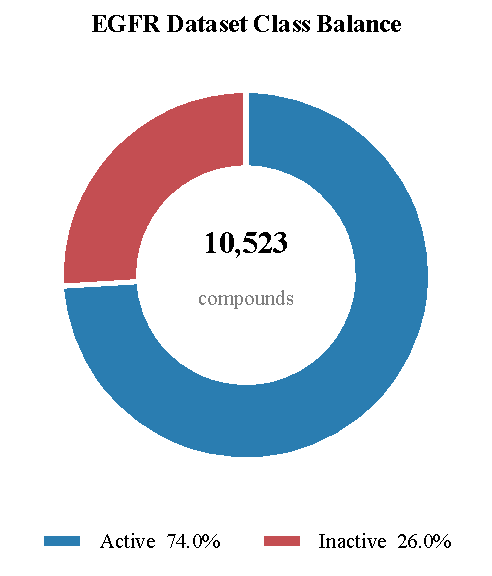
\includegraphics[width=0.5\textwidth]{eda_class_balance.pdf}
\caption{Class balance of the curated EGFR dataset: 74.0\% active and 26.0\%
         inactive compounds across 10,523 unique molecules.}
\label{fig:class_balance}
\end{figure}

\subsection{\texorpdfstring{pIC$_{50}$}{pIC50} Distribution}

The pIC$_{50}$ distribution across the full dataset exhibited a bimodal profile.
The active subpopulation was centred around $\text{pIC}_{50} \approx 7.5$--8.0
(corresponding to IC$_{50}$ values of 10--32 nM), reflecting the high-potency
compounds typically selected for further optimisation in medicinal chemistry
campaigns. The inactive subpopulation showed a peak near $\text{pIC}_{50} \approx
5.2$--5.5, representing weak binders at the micro-molar level. The binary threshold
at pIC$_{50} = 6.0$ (IC$_{50} = 1~\mu$M) was placed in a relatively low-density
valley between these two modes, providing a chemically meaningful separation rather
than an arbitrary cut-point. This is consistent with the standard medicinal chemistry
convention that defines a ``hit'' as a compound with measurable activity at or
below 1 $\mu$M. The bimodal structure and the placement of the decision threshold
are shown in Figure~\ref{fig:pic50}.

\begin{figure}[htbp]
\centering
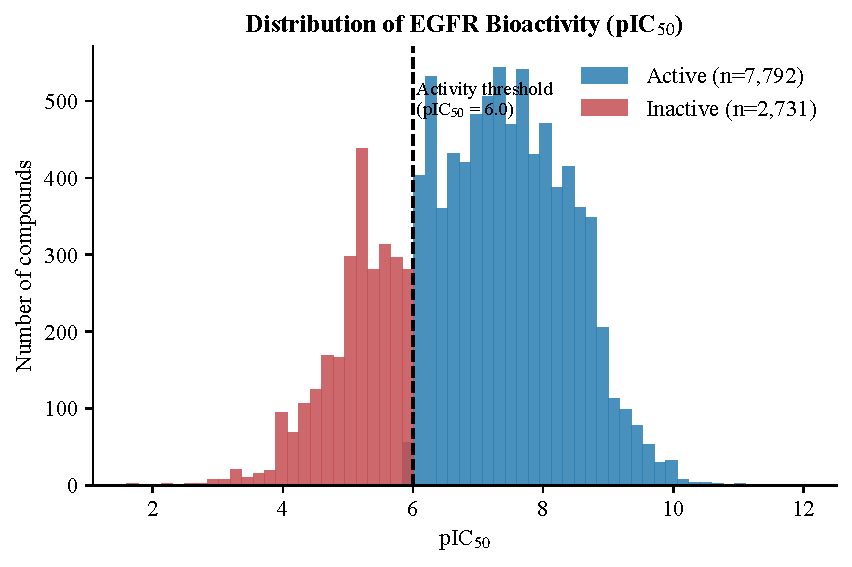
\includegraphics[width=0.82\textwidth]{eda_pic50_distribution.pdf}
\caption{Distribution of pIC$_{50}$ for the curated dataset; the two activity modes are split by the pIC$_{50}=6.0$ (1~$\mu$M) threshold (dashed).}
\label{fig:pic50}
\end{figure}

\subsection{Physicochemical Property Analysis}

Analysis of the RDKit-computed physicochemical properties of the curated dataset
revealed that the majority of compounds occupied drug-like chemical space. Key
observations are summarised in Table~\ref{tab:physchem}.

\begin{table}[H]
\centering
\caption{Summary statistics of physicochemical properties of the curated dataset.}
\label{tab:physchem}
{\singlespacing
\begin{tabular}{lcccc}
\toprule
\textbf{Property} & \textbf{Min} & \textbf{Median} & \textbf{Mean} & \textbf{Max} \\
\midrule
Molecular Weight (Da) & 65.4  & 478.0  & 475.0  & 991.7 \\
LogP                  & $-$2.0 & 4.5   & 4.5    & 13.1  \\
H-Bond Donors         & 0      & 2      & 2.2    & 10    \\
H-Bond Acceptors      & 0      & 7      & 6.6    & 17    \\
TPSA (\AA$^{2}$)      & 0.0    & 96.3   & 95.2   & 273.0 \\
\bottomrule
\end{tabular}
}
\end{table}

The median molecular weight of 478 Da and median LogP of 4.5 sit close to the upper
limits of Lipinski's Rule of Five (Ro5), consistent with the physicochemical
characteristics of ATP-competitive kinase inhibitors, which frequently occupy the
upper boundary of drug-like chemical space. Approximately \textbf{47\%} of the
compounds were fully Lipinski-compliant (MW $\leq$ 500 Da, LogP $\leq$ 5,
HBD $\leq$ 5, HBA $\leq$ 10); the remainder most often exceed the LogP or molecular
weight thresholds, reflecting the lipophilic, higher-mass character typical of this
inhibitor class. The molecular weight and lipophilicity distributions are shown in
Figure~\ref{fig:properties}.

\begin{figure}[htbp]
\centering
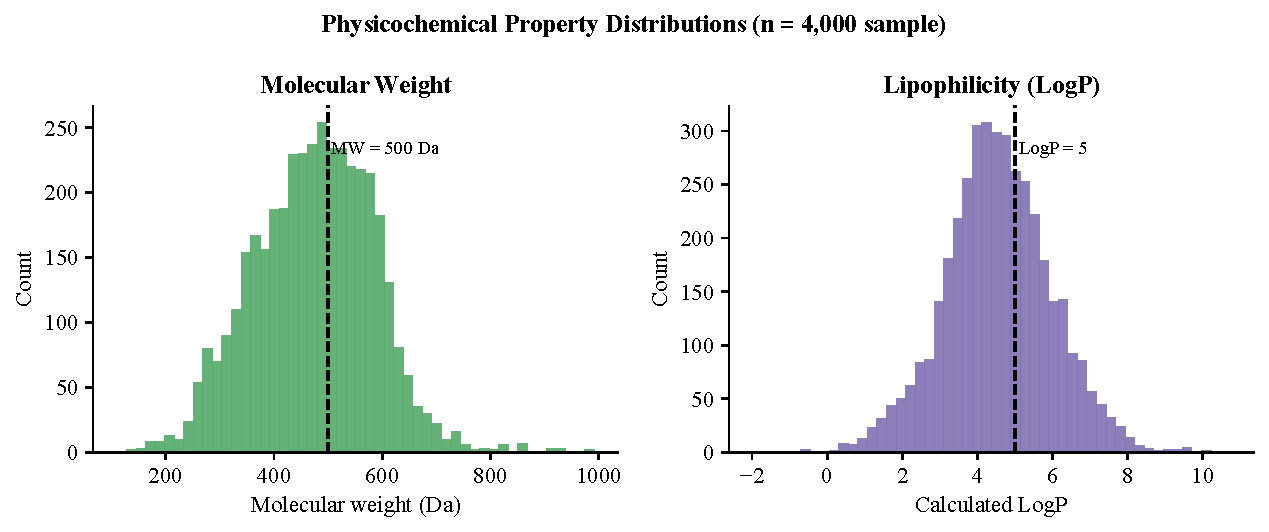
\includegraphics[width=0.95\textwidth]{eda_property_distributions.pdf}
\caption{Molecular weight (left) and LogP (right) distributions for the curated dataset; dashed lines mark the Lipinski thresholds (500~Da, 5).}
\label{fig:properties}
\end{figure}

\subsection{Scaffold Diversity Analysis}

The Bemis-Murcko scaffold analysis identified \textbf{3,693 unique scaffolds}
across the full dataset. Of these, 2,418 (65.5\%) were singletons, comprising
only a single compound. The most frequently occurring scaffold, observed in
572 compounds, corresponds to the 4-anilinoquinazoline core, which is the
defining pharmacophore of first- and second-generation EGFR TKIs including
gefitinib, erlotinib, and lapatinib. Several further scaffolds each comprising
over one hundred compounds include the pyrrolopyrimidine core characteristic of
certain second-generation and third-generation inhibitors. This scaffold-level analysis
confirms that the dataset represents a structurally diverse yet pharmacophore-focused
chemical space. Figure~\ref{fig:scaffold} shows the most frequent scaffolds and the
overall split between singleton and multi-compound scaffolds, which motivates the
use of scaffold-based data splitting.

\begin{figure}[htbp]
\centering
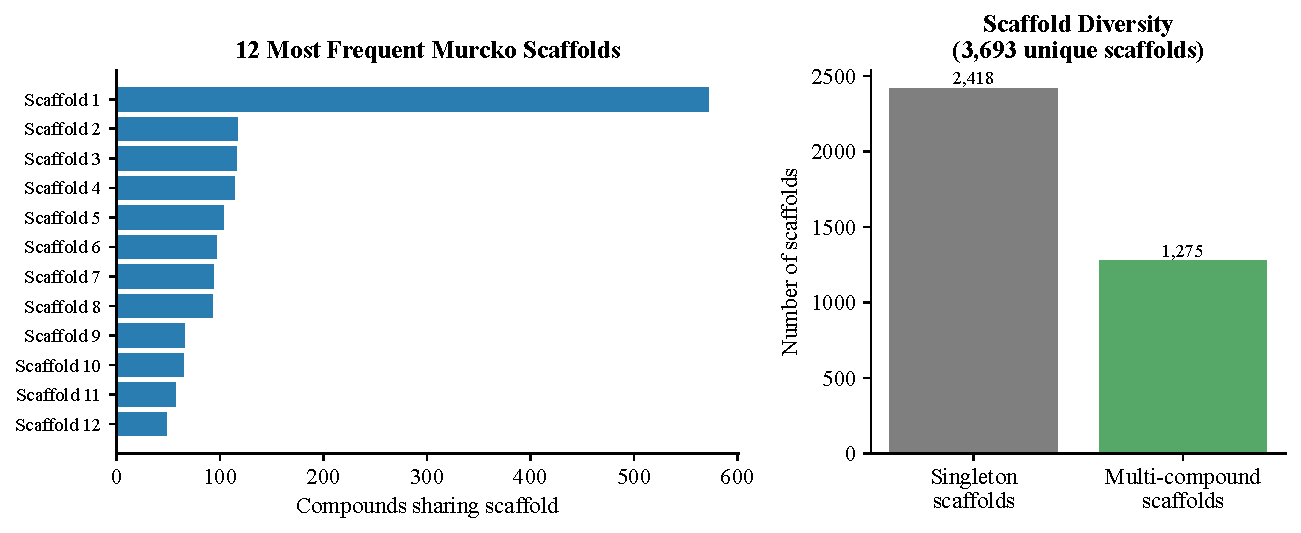
\includegraphics[width=0.95\textwidth]{eda_scaffold_diversity.pdf}
\caption{Bemis-Murcko scaffold diversity: most frequent scaffolds (left) and the singleton vs.\ multi-compound split (right).}
\label{fig:scaffold}
\end{figure}

% ----------------------------------------------------------------
\section{Machine Learning Model Performance}
\label{sec:ml_perf}
% ----------------------------------------------------------------

\subsection{Individual Model Performance on the Scaffold Test Set}

All seven models were trained under identical scaffold split conditions and evaluated
on the held-out scaffold test set of 1,053 compounds. Results are presented in
Table~\ref{tab:results}. The classification threshold was set at $\hat{p} = 0.5$
for all threshold-dependent metrics (F1-Score, MCC, Accuracy).

\begin{table}[H]
\centering
\caption{Performance comparison of all models on the scaffold-held-out test set
         (threshold = 0.50 for F1, MCC, Accuracy).}
\label{tab:results}
{\singlespacing
\begin{tabular}{llccccc}
\toprule
\textbf{Model} & \textbf{Type} & \textbf{AUROC} & \textbf{AUPRC}
               & \textbf{F1} & \textbf{MCC} & \textbf{Accuracy} \\
\midrule
\rowcolor{tableblue}
Random Forest       & ML + ECFP4 & 0.8827 & 0.9496 & 0.8762 & 0.5072 & 0.8129 \\
MLP                 & ML + ECFP4 & 0.8547 & 0.9354 & 0.8629 & 0.5281 & 0.8053 \\
GCN                 & GNN        & 0.8454 & 0.9332 & 0.7877 & 0.4707 & 0.7312 \\
GraphSAGE           & GNN        & 0.8229 & 0.9179 & 0.8070 & 0.4706 & 0.7474 \\
GIN                 & GNN        & 0.8217 & 0.9163 & 0.8487 & 0.4865 & 0.7863 \\
GAT                 & GNN        & 0.8162 & 0.9176 & 0.7689 & 0.4473 & 0.7123 \\
AttentiveFP         & GNN        & 0.8087 & 0.9108 & 0.8254 & 0.3989 & 0.7521 \\
\bottomrule
\end{tabular}
}
\end{table}

Figure~\ref{fig:model_comparison} visualises these results across the four headline
metrics, making the relative ordering of the seven models directly comparable.

\begin{figure}[htbp]
\centering
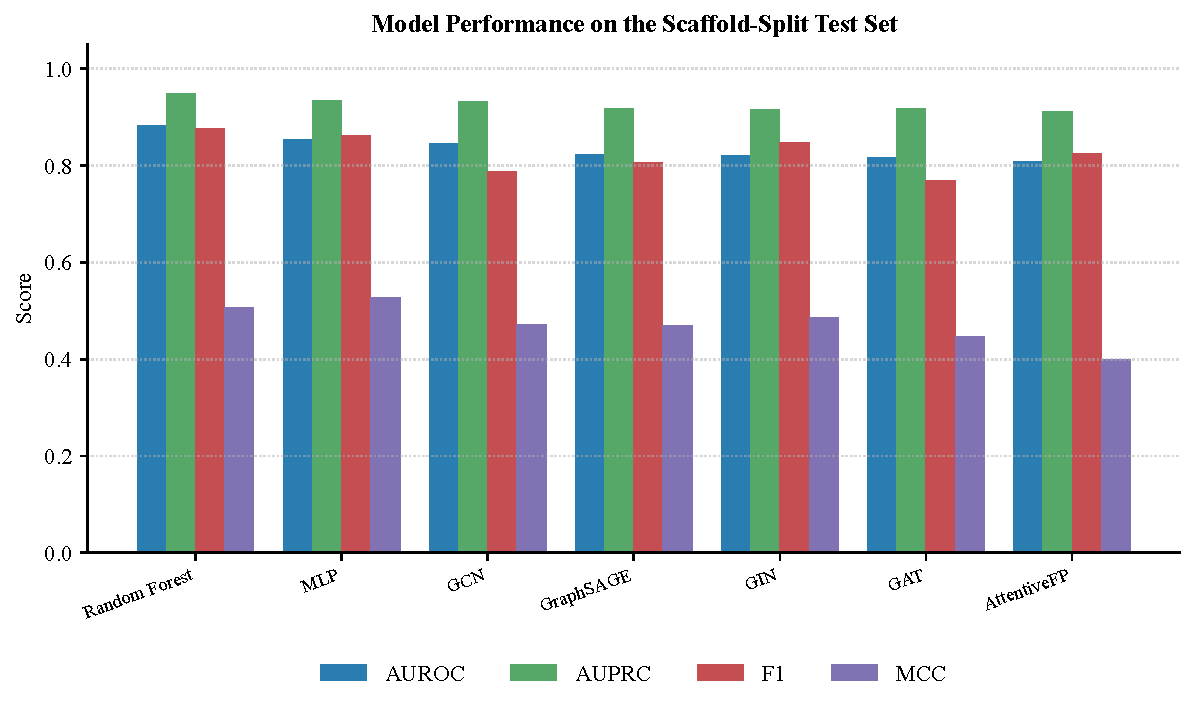
\includegraphics[width=0.98\textwidth]{results_model_comparison.pdf}
\caption{Performance of all seven models on the scaffold test set; fingerprint baselines lead, with GCN strongest among the GNNs.}
\label{fig:model_comparison}
\end{figure}

\subsubsection{Random Forest Performance}

Random Forest achieved the highest test-set AUROC (0.8827) and AUPRC (0.9496)
among all models, together with the strongest F1-Score (0.8762); the MLP baseline
attained the highest MCC (0.5281), narrowly ahead of Random Forest (0.5072). The
strong performance of the two fingerprint-based baselines is consistent with
established observations in cheminformatics benchmarks: ensemble and shallow
neural methods built on ECFP4 fingerprints are highly competitive on bioactivity
datasets of this scale ($\sim$10,000 compounds), particularly when the training
and test chemical spaces share fingerprint-level structural similarity. The high
AUPRC value (0.9496) is especially significant given the 74:26 class imbalance,
indicating that Random Forest maintains high precision at high recall thresholds.

\subsubsection{Graph Neural Network Performance}

Among the five GNN architectures at default settings, \textbf{GCN achieved the
highest AUROC (0.8454)}, followed by GraphSAGE (0.8229), GIN (0.8217), GAT
(0.8162), and AttentiveFP (0.8087). Notably, the simpler convolution- and
sampling-based architectures outperformed the more elaborate attention-based
models on this metric---a common observation, since high-capacity,
molecule-specific architectures such as AttentiveFP are highly sensitive to
hyperparameter choices and tend to underperform simpler models until properly
tuned (Section~\ref{sec:hp_tuning}). The per-architecture characteristics are:
\begin{itemize}
    \item \textbf{GCN} provided the strongest and most stable default GNN, its
          degree-normalised convolution generalising well to novel scaffolds without
          extensive tuning.
    \item \textbf{GraphSAGE} performed comparably (AUROC 0.8229), with its
          concatenated self-and-neighbour update giving robust inductive
          generalisation on molecular graphs of this scale.
    \item \textbf{GIN} achieved the strongest F1-Score (0.8487) and MCC (0.4865)
          among the GNNs; its sum aggregation preserves neighbourhood multiset
          information that benefits threshold-dependent classification.
    \item \textbf{GAT} did not translate its learned attention weights into a higher
          AUROC than GCN at default settings, indicating that the additional
          parameters require tuning to pay off.
    \item \textbf{AttentiveFP}, despite its sophisticated two-level attention and
          native 12-dimensional edge-feature integration, recorded the lowest
          default AUROC (0.8087) and MCC (0.3989). This points to substantial
          untapped capacity that motivates the dedicated hyperparameter optimisation
          reported in Section~\ref{sec:hp_tuning}.
\end{itemize}

\subsubsection{GNN vs.\ Traditional ML Baselines}

The performance gap between the fingerprint baselines and all default GNN models
(AUROC difference: 0.037--0.074 relative to Random Forest) reflects a well-documented
phenomenon in molecular machine learning: GNNs require larger training datasets and
careful tuning to overcome the strong inductive bias provided by ECFP4 fingerprints.
Notably, the MLP baseline (AUROC 0.8547), which applies deep learning to the same
ECFP4 fingerprints, outperformed all five default GNN models, confirming that the
fixed fingerprint representation—rather than deep learning capacity alone—drives the
advantage of the baselines. The ECFP4 representation was refined through decades of
cheminformatics research specifically for molecular activity prediction, while GNN
architectures must learn to identify relevant substructures from first principles.
This gap is not closed by hyperparameter optimisation: tuning AttentiveFP
(Section~\ref{sec:hp_tuning}) improved its validation AUROC but left its test AUROC
essentially unchanged, so on the strict scaffold test set the fingerprint baselines
remained ahead of every graph neural network.

\subsection{Hyperparameter Tuning Results}
\label{sec:hp_tuning}

Bayesian hyperparameter optimisation was performed over 20 Optuna trials using the
Tree-structured Parzen Estimator sampler, with the objective of maximising
validation AUROC. The optimal hyperparameter configuration identified for
AttentiveFP is presented in Table~\ref{tab:optuna}.

\begin{table}[H]
\centering
\caption{Optimal AttentiveFP hyperparameters identified by Optuna Bayesian
         optimisation over 20 trials, with the resulting performance.}
\label{tab:optuna}
{\singlespacing
\begin{tabular}{lcc}
\toprule
\textbf{Hyperparameter} & \textbf{Default Value} & \textbf{Optimal Value} \\
\midrule
\texttt{hidden\_channels}  & 128   & 128                         \\
\texttt{num\_layers}       & 2     & 3                           \\
\texttt{num\_timesteps}    & 2     & 2                           \\
\texttt{dropout}           & 0.30  & 0.129                       \\
\texttt{batch\_size}       & 64    & 64                          \\
\texttt{learning\_rate}    & 0.001 & $2.61 \times 10^{-3}$       \\
\texttt{weight\_decay}     & 0.0   & $1.10 \times 10^{-5}$       \\
\midrule
\textbf{Best validation AUROC (20 trials)} & \multicolumn{2}{c}{\textbf{0.8632}} \\
\textbf{Tuned test AUROC} (cf.\ default 0.8087) & \multicolumn{2}{c}{0.7970} \\
\bottomrule
\end{tabular}
}
\end{table}

The optimisation raised the best \emph{validation} AUROC to \textbf{0.8632}, a
modest improvement that lifts AttentiveFP into the middle of the field on the
validation metric. On the held-out scaffold \emph{test} set, however, the tuned model
achieved an AUROC of only \textbf{0.7970}---essentially unchanged from the untuned
model (0.8087), still the lowest of the GNNs, and well below the Random Forest
(0.8827) and MLP (0.8547) fingerprint baselines. In other words, hyperparameter
tuning improves the validation-set fit but does not translate into better test-set
generalisation, and the gap to the fingerprint-based baselines is not closed on this
strict scaffold-split task---a realistic outcome consistent with the well-documented
difficulty of out-performing tuned fingerprint models on medium-sized bioactivity
datasets.

The selected hyperparameters are nonetheless informative:

\begin{itemize}
    \item \textbf{num\_layers = 3}: A third message-passing layer enables atoms to
          exchange information across up to three bonds, covering the spatial extent
          of most pharmacophoric motifs (the default used only two).
    \item \textbf{dropout = 0.129}: A lower dropout than the default (0.30) was
          preferred, indicating that the model benefits from retaining more of its
          representational capacity on this dataset.
    \item \textbf{learning\_rate = $2.61 \times 10^{-3}$}: A higher learning rate
          than the default ($10^{-3}$) accelerated convergence within the per-trial
          epoch budget.
    \item \textbf{weight\_decay = $1.10 \times 10^{-5}$}: A small non-zero L2 penalty
          (absent by default) provided mild regularisation against scaffold-specific
          overfitting.
    \item \textbf{hidden\_channels, num\_timesteps, and batch\_size} were retained at
          their default values (128, 2, and 64), indicating these were already
          near-optimal for the task.
\end{itemize}

% ----------------------------------------------------------------
\section{Nepali Medicinal Plant Virtual Screening Results}
\label{sec:vs_results}
% ----------------------------------------------------------------

\subsection{Screening Library Composition}

The Nepali medicinal plant screening library was assembled from the COCONUT 2.0
database by filtering for compounds annotated to seven traditional Nepali plant
species, then applying the same RDKit standardisation pipeline as the ChEMBL training
data. Filtering and standardisation returned \textbf{535 unique natural product
compounds}. Crucially, to ensure a genuinely \emph{prospective} screen, the library
was then de-duplicated against the ChEMBL bioactivity data: \textbf{eight compounds
whose canonical SMILES already appear in the ChEMBL EGFR training data} (including the flavones
\textbf{apigenin} and \textbf{kaempferol}, and \textbf{quercetin}, ellagic acid,
pyrogallol, and pyrocatechol) were removed, since these are not novel natural-product
candidates but known compounds the classifiers may already have seen during training.
This leaves \textbf{527 genuinely unseen compounds} that were screened, distributed
across the seven species as summarised in Table~\ref{tab:library_comp}.

\begin{table}[H]
\centering
\caption{Composition of the screened Nepali plant library after removing eight ChEMBL-overlapping compounds (COCONUT~2.0).}
\label{tab:library_comp}
{\singlespacing
\begin{tabular}{lcc}
\toprule
\textbf{Plant Species} & \textbf{Compound Class} & \textbf{Compounds} \\
\midrule
\textit{Nardostachys jatamansi} & Sesquiterpenes, coumarins    & 199 \\
\textit{Terminalia chebula}     & Hydrolysable tannins         & 192 \\
\textit{Tinospora cordifolia}   & Diterpenes, alkaloids        & 71 \\
\textit{Swertia chirayita}      & Xanthones, secoiridoids      & 23 \\
\textit{Berberis aristata}      & Isoquinoline alkaloids       & 19 \\
\textit{Rhododendron arboreum}  & Triterpenoids, flavonoids    & 15 \\
\textit{Ocimum sanctum}         & Phenylpropanoids, terpenoids & 8  \\
\midrule
\textbf{Total} & --- & \textbf{527} \\
\bottomrule
\end{tabular}
}
\end{table}

The library is dominated by \textit{Nardostachys jatamansi} (199 compounds) and
\textit{Terminalia chebula} (192), reflecting their extensive phytochemical
characterisation in COCONUT, whereas \textit{Ocimum sanctum} (8) and
\textit{Rhododendron arboreum} (15) are comparatively under-represented---an
illustration of the uneven database coverage of Nepali medicinal flora. The
distribution across the seven species is shown in Figure~\ref{fig:library_comp}.

\begin{figure}[htbp]
\centering
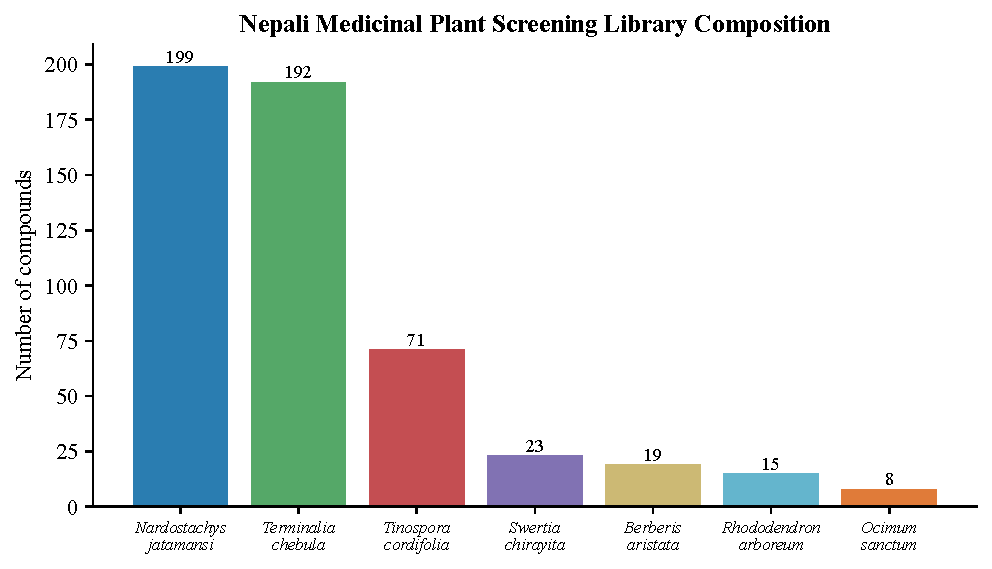
\includegraphics[width=0.9\textwidth]{screening_library_composition.pdf}
\caption{Screened Nepali plant library by species (527 genuinely unseen compounds; 535 retrieved minus eight in ChEMBL).}
\label{fig:library_comp}
\end{figure}

\subsection{Physicochemical Distribution of the Screening Library}
\label{sec:coconut_dist}

Before scoring, the physicochemical property distribution of the 527-compound COCONUT
library was characterised and compared against the ChEMBL EGFR training set of
Section~\ref{sec:data_dist}, because the two distributions determine how far the
classifiers must \emph{extrapolate}. The comparison is summarised in
Table~\ref{tab:coconut_physchem} and visualised in Figure~\ref{fig:coconut_dist}.

\begin{table}[H]
\centering
\caption{Physicochemical profile of the 527-compound Nepali library versus the 10,523-compound ChEMBL training set.}
\label{tab:coconut_physchem}
{\singlespacing
\begin{tabular}{lcc}
\toprule
\textbf{Property (median)} & \textbf{COCONUT library (527)} & \textbf{ChEMBL training (10,523)} \\
\midrule
Molecular weight (Da) & 341.4 & 478.0 \\
LogP                  & 2.5   & 4.5   \\
H-bond donors         & 2     & 2     \\
H-bond acceptors      & 4     & 7     \\
TPSA (\AA$^{2}$)      & 66.8  & 96.3  \\
QED                   & 0.4   & 0.4   \\
\midrule
Lipinski-compliant (\%) & 53.7 & 46.6 \\
\bottomrule
\end{tabular}
}
\end{table}

The natural-product library is chemically distinct from the training data on every
size- and polarity-related axis. Its median molecular weight (341.4~Da) is
\textbf{137~Da lighter} than the ChEMBL median (478.0~Da), its median LogP (2.5) is a
\textbf{full two log-units less lipophilic} (4.5), and its median TPSA (66.8~\AA$^2$)
is substantially lower (96.3~\AA$^2$). A larger fraction of the natural products are
fully Lipinski-compliant (53.7\% vs.\ 46.6\%), consistent with the generally lower
molecular weight of plant secondary metabolites relative to optimised synthetic
inhibitors. Figure~\ref{fig:coconut_dist} shows that the two molecular-weight and
lipophilicity distributions overlap only partially: the COCONUT library carries a
pronounced low-mass, low-LogP shoulder (small terpenoids and phenylpropanoids) that is
essentially absent from the training set, while also retaining a tail of very large
(MW $>900$~Da) hydrolysable tannins from \textit{Terminalia chebula}.

This distribution shift is the mechanistic explanation for the over-confidence
documented later in this section: the classifiers were trained almost entirely on
heavier, more lipophilic quinazoline-type inhibitors and must \emph{extrapolate} to
score the lighter, more polar natural products, so their predicted probabilities on
this library are not calibrated and must be treated as rankings rather than
calibrated likelihoods.

\begin{figure}[htbp]
\centering
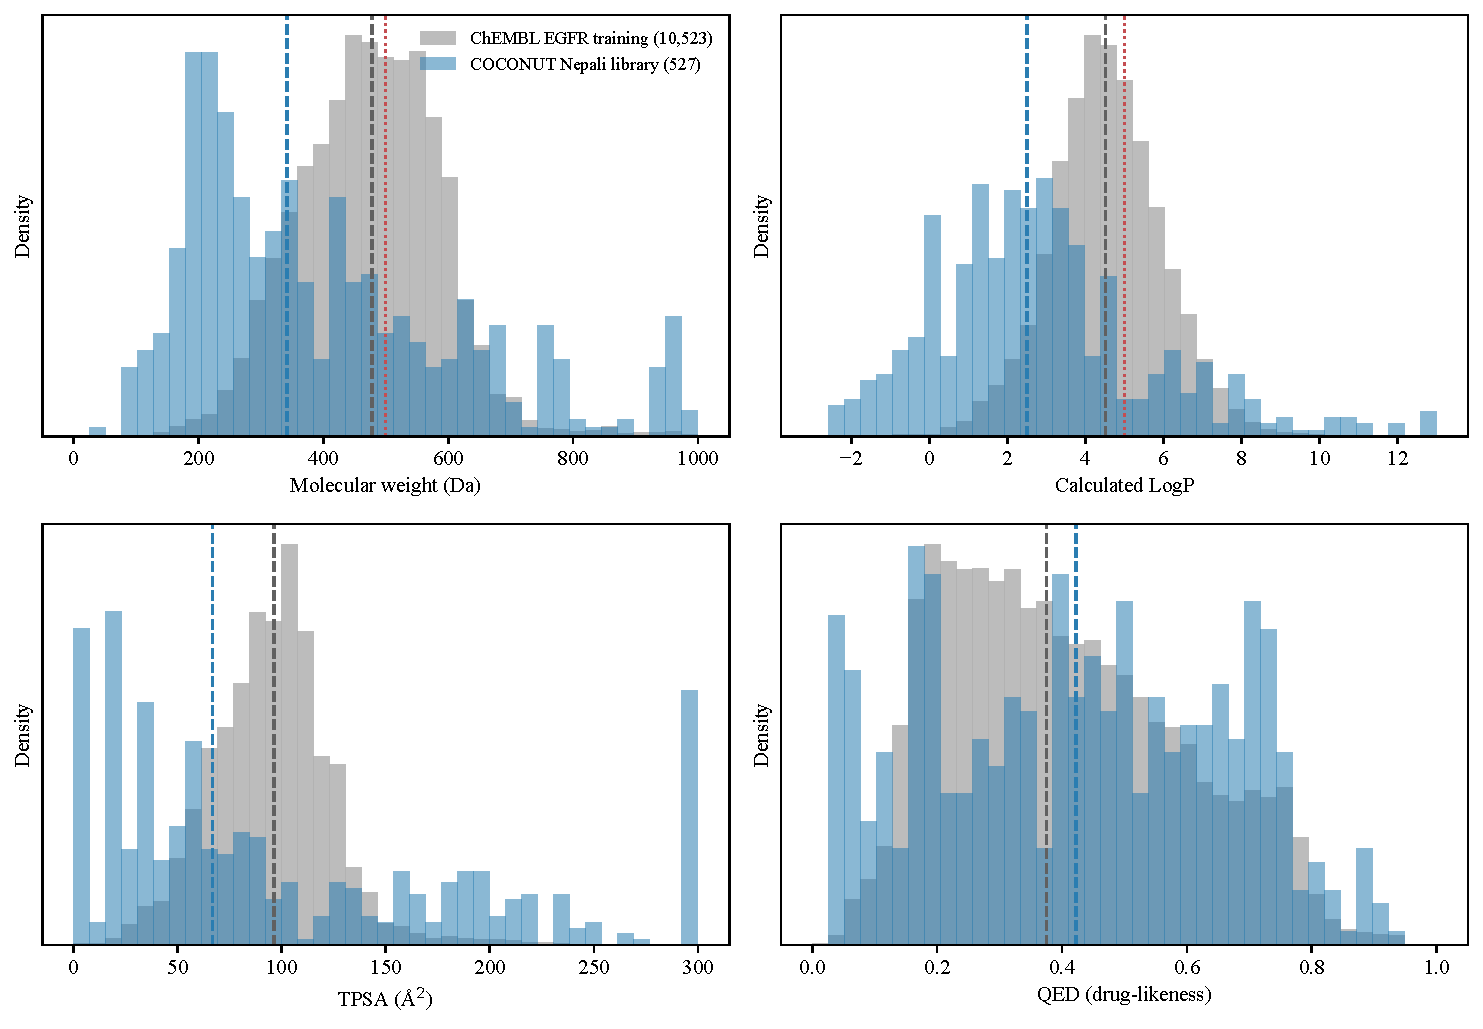
\includegraphics[width=0.98\textwidth]{coconut_distribution.pdf}
\caption{Physicochemical distributions (MW, LogP, TPSA, QED) of the Nepali library (blue) versus the ChEMBL training set (grey); dashed lines mark medians.}
\label{fig:coconut_dist}
\end{figure}

\subsection{Multi-Model Screening Funnel and Hit Identification}

A preliminary screen scored the library with the tuned AttentiveFP model. However,
AttentiveFP was in fact the \emph{weakest} classifier on the scaffold test set
(Section~\ref{sec:ml_perf}). To avoid basing lead selection on the weakest model,
the prospective screen was re-run and deployed with the study's two
\emph{best-performing} models---the strongest graph neural network (GCN, test AUROC
0.8454) and the strongest overall classifier (Random Forest, test AUROC 0.8827)---applied
to the identical 527-compound de-duplicated library. Table~\ref{tab:vs_summary}
compares the progressive screening funnel obtained under all three models.

\begin{table}[H]
\centering
\caption{Nepali plant screening funnel under the three models, showing compounds retained at each activity and drug-likeness stage.}
\label{tab:vs_summary}
{\singlespacing
\begin{tabular}{lccc}
\toprule
\textbf{Filter Stage} & \textbf{AttentiveFP} & \textbf{GCN} & \textbf{Random Forest} \\
                      & \textbf{(0.81)}      & \textbf{(0.85)} & \textbf{(0.88)} \\
\midrule
Screened compound library (de-duplicated)       & 527 & 527 & 527 \\
Predicted active ($\hat{p} \geq 0.50$)          & 143 &  24 & 179 \\
Predicted active ($\hat{p} \geq 0.80$)          &  83 &   1 &   4 \\
Predicted active ($\hat{p} \geq 0.90$)          &  71 &   0 &   0 \\
Drug-like leads ($\hat{p} \geq 0.90$, Ro5, QED $\geq 0.40$) & 11 & 0 & 0 \\
\bottomrule
\end{tabular}
}
\end{table}

The three funnels differ dramatically, and this divergence is itself a central
result. The tuned AttentiveFP predicts 143 actives at $\hat{p} \geq 0.50$ and an
implausible 71 compounds at $\hat{p} \geq 0.90$; the best graph network (GCN)
predicts only 24 actives and \emph{not a single} compound at $\hat{p} \geq 0.90$;
and the best overall classifier (Random Forest) predicts 179 actives but, on the
genuinely unseen library, likewise \emph{no} compound at $\hat{p} \geq 0.90$.
Consequently, once the eight ChEMBL-overlapping compounds are removed, \emph{neither}
best model yields a high-confidence ($\hat{p} \geq 0.90$) drug-like lead---the single
Random Forest hit above $\hat{p} \geq 0.90$ in a preliminary run was apigenin, a
compound already present in the training data (see Section~\ref{sec:disc}). The
abundance of apparently high-confidence hits in the AttentiveFP screen is therefore an
artefact of poor probability calibration on out-of-distribution natural products by
the weakest model, and is \emph{not} reproduced by either best-calibrated model. This
model-sensitivity is the principal caution of the screening campaign: virtual-screening
hit lists on natural-product chemical space depend strongly on the choice of
classifier, and the most trustworthy leads are those nominated by the strongest
models---ideally by more than one. A second, related artefact---over-confidence on
large, non-drug-like natural products---persists across models: AttentiveFP scored
large hydrolysable \textit{Terminalia chebula} tannins (e.g., pentagalloylglucose,
MW $\approx 941$~Da) at $\hat{p} \approx 1.0$, and both the GCN and the Random Forest
assigned their highest raw scores to large \textit{Swertia} and \textit{Tinospora}
triterpenoids that violate the Rule of Five, reinforcing the need to couple activity
prediction with drug-likeness filtering. The three funnels are compared in
Figure~\ref{fig:funnel}.

\begin{figure}[htbp]
\centering
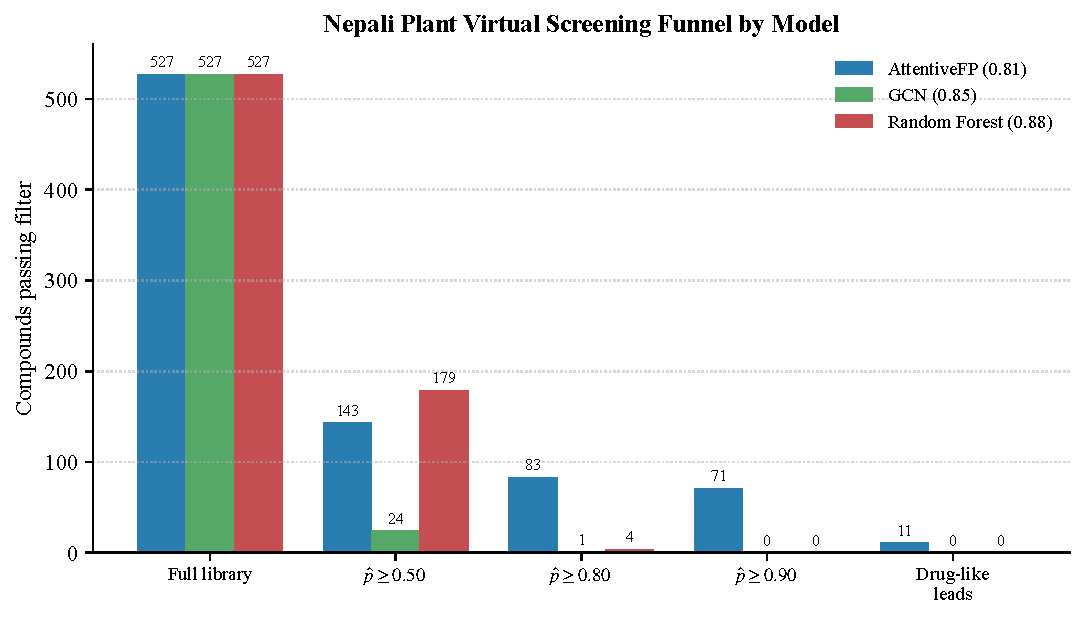
\includegraphics[width=0.9\textwidth]{screening_funnel.pdf}
\caption{Screening funnel under the three models (tuned AttentiveFP, GCN, Random Forest); the sharp disagreement shows the screen's model-sensitivity.}
\label{fig:funnel}
\end{figure}

\subsection{Consensus Leads from the Best-Performing Models}

Because no single classifier is authoritative, lead prioritisation is based on the
two best-performing models rather than the weak AttentiveFP screen. The top drug-like
(Lipinski-compliant) leads nominated by the Random Forest are listed in
Table~\ref{tab:leads_rf}, and those nominated by the GCN in Table~\ref{tab:leads_gcn}.

\begin{table}[H]
\small
\centering
\caption{Top drug-like genuinely-unseen Nepali leads under the Random Forest, ranked by predicted activity; none reaches $\hat{p}\geq0.80$.}
\label{tab:leads_rf}
{\singlespacing
\begin{tabular}{clcccccc}
\toprule
\textbf{Rank} & \textbf{Compound} & \textbf{$\hat{p}$}
              & \textbf{MW (Da)} & \textbf{LogP} & \textbf{QED}
              & \textbf{Ro5} & \textbf{Plant} \\
\midrule
1 & Isogentisin    & 0.7282 & 258.2 & 2.37 & 0.655 & $\checkmark$ & \textit{S.~chirayita}  \\
2 & Luteolin       & 0.6789 & 286.2 & 2.28 & 0.511 & $\checkmark$ & \textit{T.~chebula}    \\
3 & Tinosporaside  & 0.6607 & 492.5 & 0.63 & 0.440 & $\checkmark$ & \textit{T.~cordifolia} \\
4 & Columbin       & 0.6180 & 358.4 & 2.53 & 0.613 & $\checkmark$ & \textit{T.~cordifolia} \\
5 & Palmarin       & 0.6042 & 374.4 & 1.74 & 0.591 & $\checkmark$ & \textit{T.~cordifolia} \\
6 & Nardostachysin & 0.5836 & 430.5 & 2.95 & 0.526 & $\checkmark$ & \textit{N.~jatamansi}  \\
\bottomrule
\end{tabular}
}
\end{table}

\begin{table}[H]
\small
\centering
\caption{Top drug-like Nepali leads under the GCN, ranked by predicted activity; none reaches $\hat{p}\geq0.80$.}
\label{tab:leads_gcn}
{\singlespacing
\begin{tabular}{clcccccc}
\toprule
\textbf{Rank} & \textbf{Compound} & \textbf{$\hat{p}$}
              & \textbf{MW (Da)} & \textbf{LogP} & \textbf{QED}
              & \textbf{Ro5} & \textbf{Plant} \\
\midrule
1 & Rulepidadiene~A   & 0.6531 & 202.3 & 4.19 & 0.552 & $\checkmark$ & \textit{N.~jatamansi}  \\
2 & Nardostachysin    & 0.5915 & 430.5 & 2.95 & 0.526 & $\checkmark$ & \textit{N.~jatamansi}  \\
3 & Palmarin          & 0.5532 & 374.4 & 1.74 & 0.591 & $\checkmark$ & \textit{T.~cordifolia} \\
4 & Luteolin          & 0.5138 & 286.2 & 2.28 & 0.511 & $\checkmark$ & \textit{T.~chebula}    \\
5 & Jatamanvaltrate~H & 0.4995 & 442.5 & 1.70 & 0.405 & $\checkmark$ & \textit{N.~jatamansi}  \\
\bottomrule
\end{tabular}
}
\end{table}

Two observations stand out. First, the flavone scaffold is prominent among the
predicted actives, but this signal is strongly confounded by the training-set leakage
identified above (Table~\ref{tab:flavones}): the two highest-scoring flavones under the
Random Forest---apigenin ($\hat{p} = 0.913$) and kaempferol ($\hat{p} = 0.834$)---are
precisely the compounds already present in the ChEMBL training data (both labelled
active), so their high scores reflect \emph{memorisation}, not prospective prediction.
Once these are removed, \textbf{luteolin} is the only flavone that remains, and it is
predicted active ($\hat{p} \geq 0.50$) by \emph{both} best models (RF 0.679, GCN
0.514)---a genuinely unseen, consensus-supported candidate. Second, on the
de-duplicated library both the GCN and the Random Forest assign their highest raw
probabilities to large, non-drug-like \textit{Swertia} and \textit{Tinospora}
triterpenoids, so drug-likeness filtering remains essential.

\begin{table}[H]
\centering
\caption{Flavone scaffolds under the two best models with ChEMBL status; apigenin and kaempferol are leakage, luteolin the consensus lead.}
\label{tab:flavones}
{\singlespacing
\begin{tabular}{llccl}
\toprule
\textbf{Flavone} & \textbf{ChEMBL status} & \textbf{RF $\hat{p}$}
                 & \textbf{GCN $\hat{p}$} & \textbf{Retained?} \\
\midrule
Apigenin   & in training (active)     & 0.913 & 0.410 & removed (leakage)        \\
Kaempferol & in training (active)     & 0.834 & 0.320 & removed (leakage)        \\
Luteolin   & not in training set      & 0.679 & 0.514 & retained (consensus lead) \\
\bottomrule
\end{tabular}
}
\end{table}

Figure~\ref{fig:leads_scatter} positions the Random Forest drug-like leads in the
predicted-activity versus drug-likeness plane.

\begin{figure}[htbp]
\centering
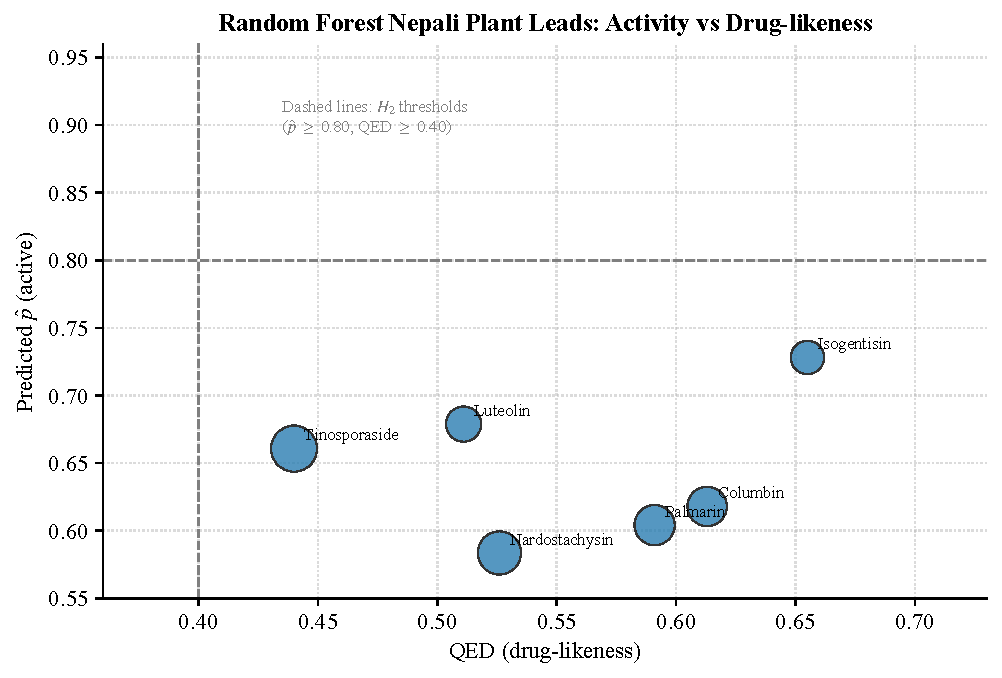
\includegraphics[width=0.92\textwidth]{screening_leads_scatter.pdf}
\caption{Random Forest drug-like leads in the predicted-activity versus QED plane; dashed lines mark the $H_2$ thresholds (0.80, 0.40), which none clears.}
\label{fig:leads_scatter}
\end{figure}

\subsubsection{Recovered Known Actives, and the Highest-Confidence Prospective Lead}

A preliminary screen of the full 535-compound library ranked two flavones
highest---apigenin ($\hat{p} = 0.913$) and kaempferol ($\hat{p} = 0.834$). Both,
however, are already present in the ChEMBL training data as known EGFR-active
compounds, so their high scores reflect the model \emph{recovering} known actives
rather than discovering new ones. Their correct recovery is a useful positive control
---the classifier does identify established EGFR-active flavones---but they are not
prospective natural-product leads, and they were removed from the screening library.

On the de-duplicated (genuinely unseen) library, \emph{no} Lipinski-compliant compound
reaches $\hat{p} \geq 0.80$ under either best model. The highest-confidence unseen
drug-like lead is \textbf{isogentisin} from \textit{Swertia chirayita}, a xanthone
scored by the Random Forest at $\hat{p} = 0.728$ (MW $= 258.2$~Da, LogP $= 2.37$,
QED $= 0.655$; fully Ro5-compliant). Isogentisin is therefore a
\emph{moderate}-confidence candidate only, and---like all leads reported here---requires
experimental validation.

\subsubsection{Cross-Model Consensus Leads and Their Plant Sources}

Because the two best models disagree so strongly, the most defensible lead-selection
criterion is \emph{cross-model consensus}: compounds predicted drug-like \emph{and}
active ($\hat{p} \geq 0.50$, Lipinski-compliant, QED $\geq 0.40$) by \emph{both} the
Random Forest and the GCN. This intersection is deliberately conservative---it discards
any lead that only one model favours, and is therefore robust to the model-sensitivity
and out-of-distribution over-confidence documented above. As Figure~\ref{fig:consensus}
shows, of the 25 drug-like actives nominated by the Random Forest and the four by the
GCN, only \textbf{three} are endorsed by both.

\begin{figure}[htbp]
\centering
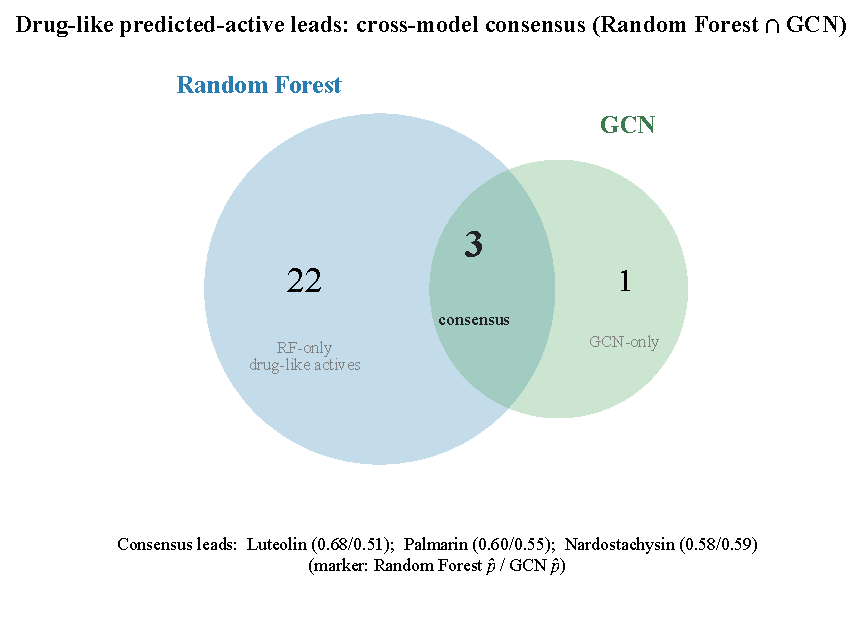
\includegraphics[width=0.78\textwidth]{screening_consensus_venn.pdf}
\caption{Cross-model consensus: drug-like actives from the Random Forest (25) and GCN (4); three (luteolin, palmarin, nardostachysin) fall in the intersection.}
\label{fig:consensus}
\end{figure}

These three consensus leads are drawn from three \emph{different} Nepali species
(Table~\ref{tab:consensus}), each with centuries of ethnopharmacological use against
inflammatory and proliferative conditions.

\begin{table}[H]
\centering
\caption{Cross-model consensus leads predicted drug-like and active by both best models, with their Nepali plant sources.}
\label{tab:consensus}
{\singlespacing
\begin{tabular}{llcccl}
\toprule
\textbf{Compound} & \textbf{Plant (common name)} & \textbf{RF $\hat{p}$}
                  & \textbf{GCN $\hat{p}$} & \textbf{QED} & \textbf{Chemotype} \\
\midrule
Luteolin       & \textit{T.~chebula} (Haritaki)    & 0.679 & 0.514 & 0.511 & Flavone \\
Palmarin       & \textit{T.~cordifolia} (Giloy)    & 0.604 & 0.553 & 0.591 & Furanoditerpenoid \\
Nardostachysin & \textit{N.~jatamansi} (Jatamansi) & 0.584 & 0.592 & 0.526 & Sesquiterpenoid ester \\
\bottomrule
\end{tabular}
}
\end{table}

\textbf{Luteolin} (\textit{Terminalia chebula}, Haritaki)\footnote{All
compound-to-plant attributions in this section follow the organism annotations
recorded in COCONUT~2.0; luteolin is a widely distributed flavone reported across
many taxa, and is here associated with \textit{Terminalia chebula} through that
database rather than as a species-exclusive constituent.} is the top consensus lead
(RF $\hat{p} = 0.679$, GCN $\hat{p} = 0.514$; MW $= 286.2$~Da, QED $= 0.511$). It is a
3$'$,4$'$,5,7-tetrahydroxyflavone---a planar, hydroxylated flavone of exactly the class
documented as ATP-competitive kinase binder, giving it clear biological plausibility.
Crucially, luteolin is \emph{not} present in the ChEMBL training data, so, unlike the
recovered apigenin and kaempferol, it is a genuinely prospective prediction.
\textbf{Palmarin} (\textit{Tinospora cordifolia}, Giloy; RF 0.604, GCN 0.553) and
\textbf{nardostachysin} (\textit{Nardostachys jatamansi}, Jatamansi; RF 0.584, GCN
0.592) contribute a furanoditerpenoid and a sesquiterpenoid-ester scaffold
respectively---chemotypes structurally distinct from luteolin and from the synthetic
quinazoline inhibitors of the training set, and therefore distinct binding-mode
hypotheses.

That the consensus set spans three traditional species---\textit{Terminalia chebula},
\textit{Tinospora cordifolia}, and \textit{Nardostachys jatamansi}, all inexpensive and
locally accessible in Nepal---makes it an attractive, diversified starting point for
experimental testing. \textbf{Luteolin} is the single highest-priority candidate,
being both the top-ranked consensus compound and a mechanistically plausible flavone,
though its moderate ($<0.80$) probabilities mean it remains a computational hypothesis
requiring \textit{in vitro} confirmation. The three source species are shown in
Figure~\ref{fig:consensus_plants}, the corresponding compound structures in
Figure~\ref{fig:consensus_struct}, and their model predictions and physicochemical
profiles in Figure~\ref{fig:consensus_data}.

\begin{figure}[htbp]
\centering
\begin{minipage}[b]{0.32\textwidth}
  \centering
  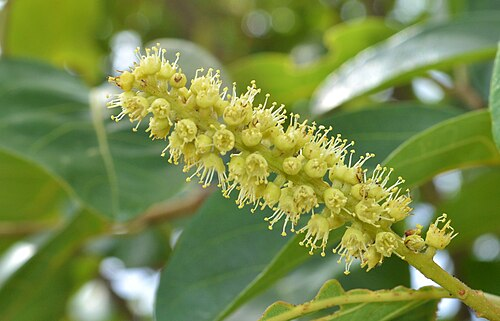
\includegraphics[height=3.2cm]{plant_terminalia.jpg}\\[2pt]
  {\small\textit{Terminalia chebula}}\\
  {\small({\nepalifont हर्रो}, Harro)}\\
  {\footnotesize\itshape luteolin}
\end{minipage}\hfill
\begin{minipage}[b]{0.32\textwidth}
  \centering
  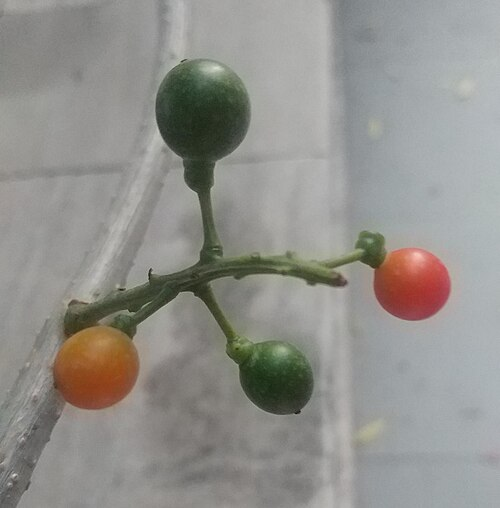
\includegraphics[height=3.2cm]{plant_tinospora.jpg}\\[2pt]
  {\small\textit{Tinospora cordifolia}}\\
  {\small({\nepalifont गुर्जो}, Gurjo)}\\
  {\footnotesize\itshape palmarin}
\end{minipage}\hfill
\begin{minipage}[b]{0.32\textwidth}
  \centering
  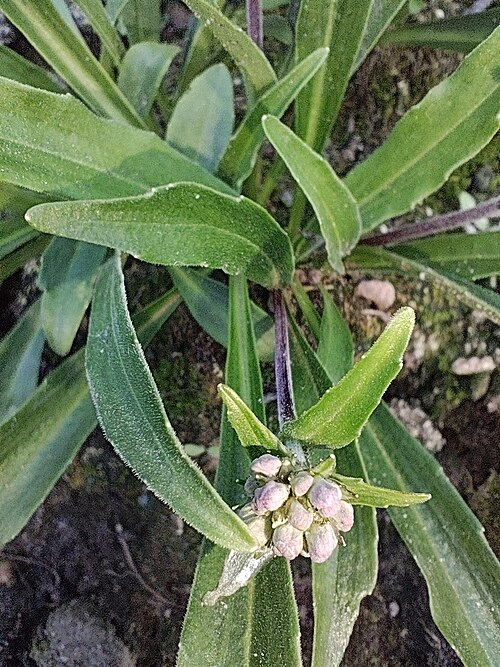
\includegraphics[height=3.2cm]{plant_nardostachys.jpg}\\[2pt]
  {\small\textit{Nardostachys jatamansi}}\\
  {\small({\nepalifont जटामसी}, Jatamasi)}\\
  {\footnotesize\itshape nardostachysin}
\end{minipage}
\caption{Consensus-lead source plants with Nepali names. Photos via Wikimedia Commons: \textit{T.~chebula} \textcopyright{} Delonix CC~BY-SA~3.0; \textit{T.~cordifolia} \textcopyright{} Gurnavinder Sidhu CC~BY-SA~4.0; \textit{N.~jatamansi} \textcopyright{} Plantagenet CC~BY-SA~4.0.}
\label{fig:consensus_plants}
\end{figure}

\begin{figure}[htbp]
\centering
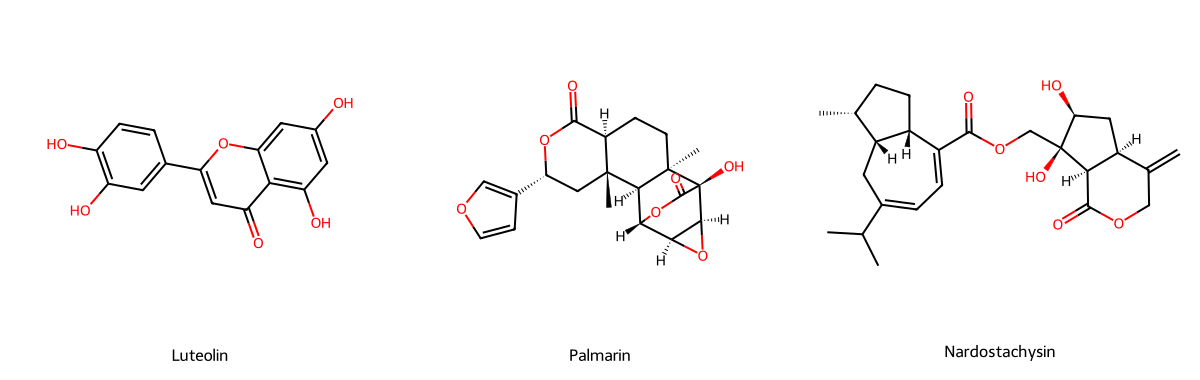
\includegraphics[width=0.95\textwidth]{consensus_structures.png}
\caption{Chemical structures of the three consensus leads (luteolin, palmarin, nardostachysin), drawn with RDKit from COCONUT~2.0 SMILES \parencite{sorokina2021coconut}.}
\label{fig:consensus_struct}
\end{figure}

\begin{figure}[htbp]
\centering
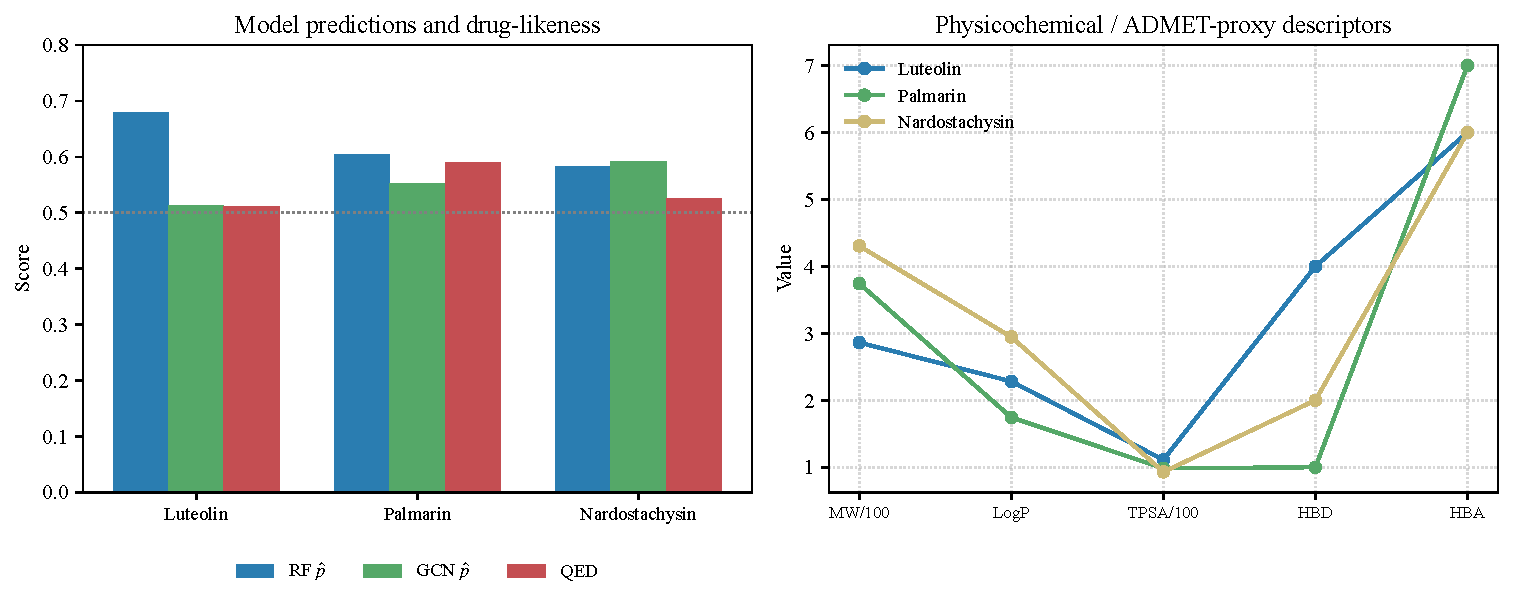
\includegraphics[width=0.98\textwidth]{consensus_data.pdf}
\caption{Model predictions and physicochemical descriptors of the three consensus leads; all satisfy Lipinski's rule of five.}
\label{fig:consensus_data}
\end{figure}

\subsection{Structural Diversity of Plant-Derived Leads}

Across the two best models the genuinely unseen drug-like leads span several distinct
chemotypes: xanthones (isogentisin), the flavone luteolin, clerodane
furanoditerpenoids (columbin, palmarin, tinosporaside), iridoid esters
(jatamanvaltrate~H, nardostachysin), and sesquiterpenoids (rulepidadiene~A). This
diversity suggests that several distinct binding modes to the EGFR ATP cleft may be
accessible from Nepali plant compounds; luteolin---the one flavone endorsed by both
best models---is the strongest single structural signal, and a richer starting point
than a structurally
homogeneous synthetic inhibitor library.

% ----------------------------------------------------------------
\section{Discussion}
\label{sec:disc}
% ----------------------------------------------------------------

\subsection{Evaluation of the Research Hypotheses}

The two research hypotheses formulated in Chapter~1 are evaluated
against the results reported above.

\textbf{$H_1$ (Performance Hypothesis) --- not supported.} $H_1$ predicted that the
graph neural networks, with rich atom and bond featurisation and Bayesian
hyperparameter optimisation, would achieve superior AUROC to the Random Forest and
MLP fingerprint baselines under the Bemis-Murcko scaffold split. The results do not
support this hypothesis: the fingerprint baselines achieved the highest scaffold
test-set AUROC (Random Forest 0.8827, MLP 0.8547), and no GNN matched them---GCN was
the strongest GNN at 0.8454, and the tuned AttentiveFP reached a validation AUROC of
only 0.8632 with a test AUROC of just 0.7970. $H_1$ is therefore
\textbf{rejected} for this dataset: on a medium-sized, scaffold-split EGFR
bioactivity set, well-tuned fingerprint models remained more accurate than the graph
neural networks. Although Bayesian optimisation was applied only to AttentiveFP
(Section~\ref{sec:hp_tuning}), this is a conservative test of $H_1$ rather than a
confound: tuning the \emph{weakest} default GNN still left it below every baseline,
while the \emph{strongest} default GNN (GCN, 0.8454) already trailed the Random Forest
by 0.037 AUROC, so closing the gap would have required the untuned architectures to
gain more from tuning than the tuned one did---an implausible margin on this dataset. This is itself an informative, honestly reported result: it directly
echoes the systematic comparison of \textcite{jiang2021gnn}, who likewise found that
descriptor-based models (including Random Forest) outperform graph-based models on
average for molecular property prediction, and is consistent with the broader
observation that ECFP4-based fingerprints are strong baselines on datasets of this
scale.

\textbf{$H_2$ (Virtual Screening Hypothesis) --- not supported.} $H_2$ predicted
that, under \emph{each} of the study's two best models, the screening pipeline would
identify at least one fully Lipinski-compliant natural-product lead with predicted
activity $\hat{p} \geq 0.80$ and QED $\geq 0.40$. A preliminary screen appeared to
satisfy this for the Random Forest (apigenin, $\hat{p} = 0.913$; kaempferol,
$\hat{p} = 0.834$), but both compounds were found to be present in the ChEMBL training
data---so their high scores are memorised known actives, not prospective predictions,
and they were removed. On the resulting genuinely unseen library, \emph{neither} best
model identifies a Lipinski-compliant compound at $\hat{p} \geq 0.80$ (Random Forest
and GCN both yield zero such leads); the highest prospective drug-like scores are
isogentisin (RF $\hat{p} = 0.728$) and luteolin (RF $0.679$, GCN $0.514$). $H_2$ is
therefore \textbf{rejected} at its stated $\hat{p} \geq 0.80$ threshold. The pipeline
does still surface \emph{moderate}-confidence, drug-like, cross-model consensus
candidates (luteolin foremost) that are worth experimental follow-up, but it does not
deliver the high-confidence prospective lead that $H_2$ posited---an honestly reported
outcome once training-set leakage is properly excluded.

\subsection{Performance of Graph Neural Networks Relative to Baselines}

The results demonstrate that the relationship between GNN and traditional ML
performance is nuanced. Across both the default and tuned configurations, the
fingerprint-based baselines outperformed all GNN models on the scaffold test set
(Random Forest AUROC 0.8827 and MLP 0.8547, versus 0.8087--0.8454 for the GNNs).
This finding is consistent with the molecular machine learning literature and
reflects two factors: (i) ECFP4 fingerprints encode decades of human cheminformatics
knowledge through their circular neighbourhood construction, providing a strong
structural inductive bias; and (ii) medium-sized bioactivity datasets ($\sim$10,000
compounds) often favour sample-efficient ensemble methods over parameter-intensive
deep learning approaches.

Bayesian hyperparameter optimisation raised AttentiveFP's validation AUROC to
0.8632 (mid-field on the validation metric), but its tuned scaffold test AUROC
(0.7970) remained the lowest of the GNNs and well below the fingerprint baselines. On this dataset, therefore, the GNNs offered no accuracy advantage: the
Random Forest was the strongest classifier and, in the prospective screen, also the
better-calibrated scoring model. The value of the graph approach here is not superior
accuracy but a genuinely independent representation---operating directly on molecular
graphs with the 29-dimensional atomic node features and 12-dimensional edge features
that are invisible to ECFP4 fingerprints---which lets the best GNN (GCN) serve as a
complementary second opinion to the Random Forest and thereby supports the cross-model
consensus prioritisation used in the screen that follows.

\subsection{Significance of Scaffold-Based Evaluation}

A critical methodological contribution of this thesis is the strict application of
Bemis-Murcko scaffold splitting. This approach fundamentally differs from random
splitting, which can lead to optimistic performance estimates when structurally
similar molecules appear in both training and test sets. Under scaffold splitting,
the test set is composed entirely of compound-scaffold pairs whose core frameworks
were never seen during training, providing a stringent evaluation of the model's
ability to generalise to genuinely novel chemical matter.

\subsection{Ethnopharmacological Rationale for Natural Product Screening}

The hit rate observed in the Nepali plant screening was itself model-dependent,
ranging from 4.6\% (GCN) through 34.0\% (Random Forest) at $\hat{p} \geq 0.50$ on the
de-duplicated library. That the models recovered the known EGFR-active flavones
apigenin and kaempferol (before these were excluded as leakage), and that the sole
remaining unseen flavone---luteolin---is endorsed by both best models, is consistent
with the ethnopharmacological enrichment inherent in traditional medicinal plant
selection: plants used for centuries against inflammatory and proliferative conditions
are biologically pre-filtered for bioactive chemical space. The planar, hydroxylated flavone
scaffold can hydrogen-bond to the kinase hinge region through its ring-hydroxyl and
4-carbonyl groups---the same anchoring interaction exploited by the ATP-competitive
pharmacophore of synthetic EGFR inhibitors---and flavonoids such as quercetin are
long-established ATP-competitive kinase inhibitors, giving luteolin clear structural
plausibility as an EGFR binder (a plausibility that nonetheless requires the
\textit{in vitro} confirmation noted above).
At the same time, both the weakest model (AttentiveFP) and the best models still rank
large, non-drug-like polyphenols and triterpenoids among their highest-scoring
compounds---a reminder that predictions on chemical space distant from the training
distribution must be interpreted with caution and coupled with drug-likeness filtering.

\subsection{Lead Compound Prioritisation Strategy}

The prioritisation strategy applied four criteria---exclusion of compounds already in
the training data (to keep the screen prospective), predicted activity, Lipinski Rule
of Five compliance, and consensus between the two best models---reflecting novelty,
target-engagement potential, oral bioavailability, and robustness to the
model-sensitivity documented above. Under this strategy \textbf{luteolin} is the top
cross-model consensus lead and \textbf{isogentisin} the highest-confidence
single-model prospective lead, both at moderate confidence. Critically, these
compounds are derived from plants (\textit{Terminalia chebula}, \textit{Swertia
chirayita}) that are inexpensive, culturally familiar, and locally accessible
throughout Nepal, offering a potential pathway to affordable candidate compounds
without the high synthesis costs of novel synthetic scaffolds.

It is important to note that the prioritisation in this study represents an
\textit{in silico} hypothesis, not experimental confirmation. The identified leads
require: (i) \textit{in vitro} EGFR kinase inhibition assay; (ii) cellular
antiproliferative testing in EGFR-mutant NSCLC cell lines (e.g., PC9, HCC827);
and (iii) selectivity profiling against a kinase panel.

\subsection{Limitations of the Current Results}

Several limitations of the results presented in this chapter should be acknowledged:

\begin{itemize}
    \item \textbf{Model-sensitivity of the screen}: The single most important
          limitation is that the virtual-screening hit list depends strongly on the
          choice of classifier (143 predicted actives for AttentiveFP versus 24 for
          GCN and 179 for Random Forest at $\hat{p} \geq 0.50$; 71 versus 0 versus 0
          at $\hat{p} \geq 0.90$). No single model can be treated as authoritative,
          and the predicted probabilities are not calibrated on out-of-distribution
          natural products. Consensus across the best models mitigates but does not
          eliminate this uncertainty; only experimental assay can resolve it.
    \item \textbf{Train/screen overlap (leakage)}: Eight of the 535 retrieved
          COCONUT compounds---including the apparent top hits apigenin and
          kaempferol---were already present in the ChEMBL training data as known
          actives. These were excluded so that the reported screen is genuinely
          prospective, but their presence shows that natural-product libraries can
          overlap curated bioactivity databases, and that such overlap must be removed
          before any prospective claim; a screen that omits this step would badly
          overstate its ``discoveries.''
    \item \textbf{Validation AUROC vs.\ Test AUROC}: The tuned AttentiveFP's
          validation AUROC (0.8632) exceeded its scaffold test AUROC ($\approx$0.80),
          a gap that reflects optimisation against the validation partition. Future
          work should employ a nested cross-validation scheme for unbiased test-set
          estimation.
    \item \textbf{Assay heterogeneity}: Training labels aggregate IC$_{50}$ values
          from hundreds of laboratories with different protocols, imposing a label
          noise ceiling on scaffold-split test-set performance.
    \item \textbf{ADMET-proxy limitations}: The physicochemical properties used
          do not capture metabolic stability, P-glycoprotein efflux, plasma protein
          binding, or \textit{in vivo} pharmacokinetics.
    \item \textbf{COCONUT 2.0 annotation completeness}: Organism taxonomy annotations
          in COCONUT 2.0 may be incomplete for some Nepali plant species, potentially
          missing additional bioactive compounds from these plants.
    \item \textbf{No 3D structural validation}: The absence of molecular docking
          against EGFR crystal structures means no binding pose or free energy
          estimate is available to corroborate model predictions for the top leads.
\end{itemize}
\chapter{Conclusions and Recommendations}

\section{Conclusions}

This thesis presented a comprehensive, open-source end-to-end computational
framework for the binary classification of EGFR inhibitor activity and the
prospective virtual screening of novel lead compounds for drug-resistant NSCLC.
The following principal conclusions can be drawn:

\begin{enumerate}
    \item \textbf{Data quality and curation are foundational.} Applying rigorous
          ChEMBL curation---including filtering for exact IC$_{50}$ values, pIC$_{50}$
          conversion, RDKit-based salt removal, canonicalisation, and molecular weight
          filtering---produced a high-quality, unambiguous dataset of 10,523 unique
          EGFR-bioactive compounds suitable for deep learning.

    \item \textbf{Fingerprint baselines outperformed the graph neural networks.}
          Under strict Bemis-Murcko scaffold evaluation, the Random Forest baseline
          achieved the highest test AUROC (0.8827), ahead of the MLP on ECFP4
          fingerprints (0.8547) and the five graph neural networks (0.8087--0.8454).
          Among the GNNs, GCN was strongest at default settings, while
          AttentiveFP---which natively exploits the 29-dimensional atom and
          12-dimensional bond features---required Bayesian hyperparameter optimisation
          to reach mid-field on the validation set (best validation AUROC 0.8632),
          although its test AUROC (0.7970) remained the lowest of the GNNs. These
          results show that, on a medium-sized scaffold-split EGFR dataset, well-tuned
          fingerprint models remain more accurate than graph neural networks for
          classification, and hypothesis $H_1$ is therefore \textbf{rejected}.

    \item \textbf{Nepali medicinal plant virtual screening is model-sensitive and,
          once leakage is removed, yields only moderate-confidence leads.} Of the 535
          retrieved compounds, eight---including the apparent top hits \textbf{apigenin}
          and \textbf{kaempferol}---were already present in the ChEMBL training data as
          known actives; recovering them is a positive control, not a discovery, so they
          were excluded, leaving 527 genuinely unseen compounds. On this de-duplicated
          library the two best models gave sharply different funnels (Random Forest 179
          vs.\ GCN 24 predicted actives at $\hat{p} \geq 0.50$), and \emph{neither}
          produced a Lipinski-compliant lead at $\hat{p} \geq 0.90$---exposing the
          earlier tuned-AttentiveFP screen (71 compounds above $\hat{p} \geq 0.90$) as
          over-confident. The strongest prospective candidates are the xanthone
          \textbf{isogentisin} (Random Forest $\hat{p} = 0.728$) and the flavone
          \textbf{luteolin}, the top cross-model consensus lead (both models
          $\hat{p} \geq 0.50$), both at moderate confidence. Because no best model
          reaches the $\hat{p} \geq 0.80$ bar, hypothesis $H_2$ is \textbf{rejected},
          and the leads are consensus-supported starting points for experimental
          validation rather than high-confidence hits.

    \item \textbf{Consensus across models is essential for trustworthy natural-product
          screening.} Because the predicted hit list depends strongly on the choice of
          classifier and the models are not calibrated on out-of-distribution natural
          products, no single model can be treated as authoritative. Prioritising
          compounds endorsed by more than one strong model---and coupling activity
          prediction with drug-likeness filtering, since the weaker models still
          ranked large, non-drug-like \textit{Terminalia chebula} tannins and
          \textit{Tinospora} triterpenoids among their highest scorers---is the key
          methodological lesson of the screening campaign. The flavone leads that survive this scrutiny, combined
          with the low cost and cultural accessibility of their source plants in Nepal,
          make them valuable starting points for affordable NSCLC drug discovery.

    \item \textbf{The pipeline is reproducible, scalable, and regionally relevant.}
          The entire framework uses exclusively open-source Python tools (PyTorch
          Geometric, RDKit, Optuna, scikit-learn, COCONUT 2.0) and public databases
          (ChEMBL, COCONUT), runs on commodity CPU hardware, and is immediately
          adaptable to other kinase targets or plant species without specialised
          hardware or licensed software. This makes it directly accessible to academic
          researchers in Nepal and other resource-limited South Asian settings.
\end{enumerate}

\section{Recommendations for Future Work}

\begin{enumerate}
    \item \textbf{Experimental validation of Nepali plant leads.} The top genuinely
          unseen, cross-model-consensus leads---particularly the flavone luteolin
          (\textit{Terminalia chebula}) and the xanthone isogentisin
          (\textit{Swertia chirayita})---should be subjected to \textit{in vitro} EGFR
          kinase inhibition assays and EGFR-mutant NSCLC cell line proliferation assays
          (e.g., PC9, HCC827) to validate the computational predictions empirically.
          The known actives recovered by the screen (apigenin, kaempferol) can serve as
          assay positive controls.

    \item \textbf{Mutant-specific modelling.} As mutation-specific bioactivity datasets
          for T790M and C797S EGFR grow in public databases, dedicated GNN models trained
          specifically on these mutant targets should be developed to directly address
          drug resistance.

    \item \textbf{3D graph representation.} Incorporating three-dimensional molecular
          conformations (e.g., through SchNet or DimeNet++ architectures) and protein
          structure-aware approaches could improve the prediction of binding affinity
          for specific EGFR mutant forms.

    \item \textbf{Pre-training on large molecular datasets.} Applying self-supervised
          graph pre-training on millions of unlabelled molecules (e.g., from ZINC or
          PubChem) before fine-tuning on EGFR data could further improve scaffold
          generalisation.

    \item \textbf{Broader Nepali plant species survey.} The current study covered
          seven ethnopharmacologically relevant species. A systematic expansion to the
          full catalogue of 700+ documented Nepali medicinal plants, using COCONUT 2.0
          and complementary databases (e.g., Dr.\ Duke's Phytochemical Database, NPACT),
          could identify additional EGFR inhibitor candidates from the rich Himalayan
          biodiversity.

    \item \textbf{Extended ADMET profiling.} The current ADMET analysis used RDKit
          physicochemical property proxies. Future work should incorporate dedicated
          ADMET prediction tools such as SwissADME, pkCSM, or deep ADMET models for
          comprehensive absorption, distribution, metabolism, excretion, and toxicity
          profiling of the top leads.

    \item \textbf{Collaboration with Nepal-based research institutions.} To translate
          these computational predictions into experimental evidence, partnerships should
          be established with Nepal-based pharmacology and oncology research institutions---such
          as the B.P.\ Koirala Institute of Health Sciences (BPKIHS) and the National
          Cancer Hospital and Research Centre (NCHRC)---for wet-lab assay, phytochemical
          isolation, and clinical-translational validation of the top Nepali medicinal
          plant lead compounds.
\end{enumerate}


%% ── REFERENCES ──────────────────────────────────────────────────────
\cleardoublepage
\printbibliography[heading=bibintoc,title={References}]

%% ── APPENDICES ──────────────────────────────────────────────────────
\cleardoublepage
\appendix
\renewcommand{\chaptername}{Appendix}
\addtocontents{toc}{\protect\contentsline{chapter}{\textbf{Appendices}}{}{}}
%═══════════════════════════════════════════════════════
%  APPENDICES
%═══════════════════════════════════════════════════════

%───────────────────────────────────────────────────────
%  APPENDIX A — Dataset Information
%───────────────────────────────────────────────────────
\clearpage
\section*{Appendix A: Dataset Information}
\addcontentsline{toc}{section}{Appendix A: Dataset Information}
\label{app:dataset}

\subsection*{A.1 ChEMBL Query Parameters}

The EGFR bioactivity dataset was retrieved from ChEMBL
\parencite{mendez2019chembl} via the REST API in May 2026 using the parameters
listed in Table~\ref{tab:app_chembl_query}. Only binding assay
records with high confidence scores were retained.

\begin{table}[H]
\caption{ChEMBL query parameters used to retrieve EGFR
         bioactivity data.}
\label{tab:app_chembl_query}
\centering
\begin{tabular}{@{}p{5cm}p{8cm}@{}}
\toprule
\textbf{Parameter} & \textbf{Value} \\
\midrule
Database           & ChEMBL (May 2026 release) \\
Target name        & Epidermal Growth Factor Receptor (EGFR) \\
ChEMBL target ID   & CHEMBL203 \\
Activity type      & IC\textsubscript{50} \\
Units              & nM (nanomolar) \\
Assay type         & B (binding assay) \\
Confidence score   & $\geq 9$ (direct single protein target) \\
Organism           & \textit{Homo sapiens} \\
Activity threshold & pIC\textsubscript{50} $\geq 6.0$
                     $\rightarrow$ Active
                     (IC\textsubscript{50} $\leq 1\,\mu$M);\\
                   & pIC\textsubscript{50} $< 6.0$
                     $\rightarrow$ Inactive \\
Data split method  & Bemis-Murcko scaffold split \\
\bottomrule
\end{tabular}
\end{table}

\subsection*{A.2 Dataset Curation Statistics}

Table~\ref{tab:app_curation} shows the number of compounds
retained at each stage of the curation pipeline.

\begin{table}[H]
\caption{Step-by-step dataset curation statistics for the
         EGFR bioactivity dataset.}
\label{tab:app_curation}
\centering
\begin{tabular}{@{}clc@{}}
\toprule
\textbf{Step} & \textbf{Filter Applied}
              & \textbf{Compounds Remaining} \\
\midrule
0 & Raw ChEMBL records retrieved           & $\sim$15{,}000--20{,}000 \\
1 & Remove missing or invalid SMILES       & --- \\
2 & Salt stripping and canonicalisation    & --- \\
3 & Molecular weight filter (100--1000 Da) & --- \\
4 & Remove duplicate molecules             & --- \\
\midrule
  & \textbf{Final curated dataset}         & \textbf{10{,}523} \\
\midrule
  & Active (pIC\textsubscript{50}
    $\geq 6.0$)                            & 7{,}792 (74.0\%) \\
  & Inactive (pIC\textsubscript{50}
    $< 6.0$)                              & 2{,}731 (26.0\%) \\
  & Active:Inactive ratio                 & 2.85:1 \\
\midrule
  & Training set (80\%, scaffold)         & 8{,}418 \\
  & Validation set (10\%, scaffold)       & 1{,}052 \\
  & Test set (10\%, scaffold)             & 1{,}053 \\
\bottomrule
\end{tabular}
\end{table}

\noindent
The Bemis-Murcko scaffold split ensures that all molecules
sharing the same core framework are assigned to the same
partition, preventing optimistic bias from scaffold
memorisation and providing a more realistic estimate of
generalisation to novel chemical matter.


%───────────────────────────────────────────────────────
%  APPENDIX B — Screening Library and Results
%───────────────────────────────────────────────────────
\clearpage
\section*{Appendix B: Screening Library and Virtual
          Screening Results}
\addcontentsline{toc}{section}{Appendix B: Screening
  Library and Virtual Screening Results}
\label{app:library}

\subsection*{B.1 Screening Library Source}

The virtual screening library was curated from seven traditional Nepali medicinal
plant species---\textit{Swertia chirayita}, \textit{Rhododendron
arboreum}, \textit{Nardostachys jatamansi}, \textit{Terminalia
chebula}, \textit{Berberis aristata}, \textit{Ocimum sanctum},
and \textit{Tinospora cordifolia}---retrieved from the
COCONUT~2.0 natural product database \parencite{sorokina2021coconut}
and standardised with the same RDKit pipeline as the training data.
Retrieval returned 535 compounds; \textbf{eight already present in the ChEMBL data}
(including apigenin and kaempferol) were removed as train/screen leakage, leaving
\textbf{527 genuinely unseen compounds} screened. These ethnomedicinal species are
traditionally used for inflammatory and proliferative conditions, enriching the
library for bioactive chemical space relative to random chemical libraries. The
composition of the screened library by species is given in
Table~\ref{tab:app_nepali_lib}.

\begin{table}[H]
\caption{Composition of the screened Nepali plant library by species (COCONUT~2.0).}
\label{tab:app_nepali_lib}
\centering
\begin{tabular}{@{}llc@{}}
\toprule
\textbf{Plant Species} & \textbf{Major Compound Class}
                       & \textbf{Compounds} \\
\midrule
\textit{Nardostachys jatamansi} & Sesquiterpenes, coumarins    & 199 \\
\textit{Terminalia chebula}     & Hydrolysable tannins         & 192 \\
\textit{Tinospora cordifolia}   & Diterpenes, alkaloids        & 71  \\
\textit{Swertia chirayita}      & Xanthones, secoiridoids      & 23  \\
\textit{Berberis aristata}      & Isoquinoline alkaloids       & 19  \\
\textit{Rhododendron arboreum}  & Triterpenoids, flavonoids    & 15  \\
\textit{Ocimum sanctum}         & Phenylpropanoids, terpenoids & 8   \\
\midrule
\textbf{Total} & --- & \textbf{527} \\
\bottomrule
\end{tabular}
\end{table}

All 527 unseen compounds were scored by the study's two best-performing models---the
best graph network (GCN) and the best overall classifier (Random Forest). The best
classifier predicted \textbf{179 compounds} active at $\hat{p} \geq 0.50$; on the
de-duplicated library \emph{neither} best model produced a Lipinski-compliant lead
above $\hat{p} \geq 0.80$. The highest-confidence unseen drug-like lead is
\textbf{isogentisin} (Random Forest $\hat{p} = 0.728$), and \textbf{luteolin} is the
top cross-model consensus lead (predicted active by both models).

\subsection*{B.2 Top Prospective Lipinski-Compliant Lead}

\begin{table}[H]
\caption{Canonical SMILES and physicochemical properties of the highest-confidence
         \emph{genuinely unseen} Lipinski-compliant lead (Random Forest).}
\label{tab:app_smiles}
\centering
\small
\begin{tabular}{@{}p{3.5cm}p{9.8cm}@{}}
\toprule
\textbf{Property} & \textbf{Value} \\
\midrule
Compound
  & Isogentisin \\
Source species
  & \textit{Swertia chirayita} \\
Predicted probability ($\hat{p}$, Random Forest)
  & 0.7282 \\
Predicted probability ($\hat{p}$, GCN)
  & 0.4600 \\
Canonical SMILES
  & \texttt{COc1ccc2oc3cc(O)cc(O)c3c(=O)c2c1} \\
Molecular Weight (Da)
  & 258.2 \\
LogP
  & 2.37 \\
QED
  & 0.655 \\
TPSA (\AA$^2$)
  & 79.9 \\
Lipinski Ro5 violations
  & 0 \\
Compound class
  & Xanthone (polyphenolic) \\
\bottomrule
\end{tabular}
\end{table}

\subsection*{B.3 Virtual Screening Summary Statistics}

\begin{table}[H]
\caption{Virtual screening summary for the two best models on the 527-compound Nepali library.}
\label{tab:app_vs_summary}
\centering
\begin{tabular}{@{}lcc@{}}
\toprule
\textbf{Metric} & \textbf{Random Forest} & \textbf{GCN} \\
\midrule
Total compounds screened          & 527 & 527 \\
Predicted active ($\hat{p} \geq 0.50$) & 179 (34.0\%) & 24 (4.6\%) \\
Predicted active ($\hat{p} \geq 0.75$) & 32 (6.1\%)   &  2 (0.4\%) \\
Predicted active ($\hat{p} \geq 0.90$) &  0 (0.0\%)   &  0 (0.0\%) \\
Highest-confidence compliant lead & Isogentisin & Rulepidadiene~A \\
Top consensus lead (both models)  & \multicolumn{2}{c}{Luteolin} \\
\bottomrule
\end{tabular}
\end{table}


%───────────────────────────────────────────────────────
%  APPENDIX C — GNN Architecture and Hyperparameters
%───────────────────────────────────────────────────────
\clearpage
\section*{Appendix C: GNN Architecture and
          Hyperparameter Optimisation}
\addcontentsline{toc}{section}{Appendix C: GNN Architecture
  and Hyperparameter Optimisation}
\label{app:hyperparams}

\subsection*{C.1 AttentiveFP Final Hyperparameters}

Table~\ref{tab:app_hyperparams} lists the final
hyperparameters of the tuned AttentiveFP model selected
by Bayesian optimisation using Optuna over 20 trials,
with validation AUROC as the objective.

\begin{table}[H]
\caption{Final hyperparameters of the tuned AttentiveFP
         model selected by Optuna Bayesian optimisation.}
\label{tab:app_hyperparams}
\centering
\begin{tabular}{@{}lcc@{}}
\toprule
\textbf{Hyperparameter} & \textbf{Search Range}
                        & \textbf{Optimal Value} \\
\midrule
Hidden dimension        & \{64, 128, 256\} & 128 \\
Message passing layers  & 2--4      & 3 \\
Attention timesteps ($T$) & 2--4   & 2 \\
Dropout rate            & 0.1--0.5  & 0.129 \\
Learning rate           & $10^{-4}$--$10^{-2}$ & $2.61\times10^{-3}$ \\
Batch size              & \{32, 64, 128\} & 64 \\
L2 weight decay         & $10^{-5}$--$10^{-3}$ & $1.10\times10^{-5}$ \\
Optimiser               & ---       & Adam \\
Loss function           & ---       & Binary cross-entropy \\
Training epochs         & ---       & $\leq$80 (early stopping) \\
\bottomrule
\end{tabular}
\end{table}

\subsection*{C.2 Model Performance Comparison}

Table~\ref{tab:app_model_compare} compares all five GNN
architectures and two traditional machine learning
baselines evaluated under the Bemis-Murcko scaffold split.

\begin{table}[H]
\caption{Performance comparison of GNN architectures and
         traditional ML baselines on the EGFR scaffold test set
         (Bemis-Murcko split).}
\label{tab:app_model_compare}
\centering
\begin{tabular}{@{}lcccc@{}}
\toprule
\textbf{Model} & \textbf{AUROC} & \textbf{AUPRC}
               & \textbf{F1} & \textbf{MCC} \\
\midrule
\textbf{Random Forest (ECFP4)} & \textbf{0.8827} & \textbf{0.9496} & \textbf{0.8762} & 0.5072 \\
MLP (ECFP4)                & 0.8547 & 0.9354 & 0.8629 & \textbf{0.5281} \\
GCN                        & 0.8454 & 0.9332 & 0.7877 & 0.4707 \\
GraphSAGE                  & 0.8229 & 0.9179 & 0.8070 & 0.4706 \\
GIN                        & 0.8217 & 0.9163 & 0.8487 & 0.4865 \\
GAT                        & 0.8162 & 0.9176 & 0.7689 & 0.4473 \\
AttentiveFP                & 0.8087 & 0.9108 & 0.8254 & 0.3989 \\
\bottomrule
\end{tabular}
\end{table}

\subsection*{C.3 Molecular Graph Feature Vectors}

\begin{table}[H]
\caption{Node (atom) and edge (bond) feature vectors
         used as input to all GNN architectures.}
\label{tab:app_features}
\centering
\begin{tabular}{@{}p{3cm}p{2cm}p{8cm}@{}}
\toprule
\textbf{Feature} & \textbf{Dim.} & \textbf{Description} \\
\midrule
\multicolumn{3}{l}{\textit{Node features ($d_n = 29$)}} \\
Atom type       & 10 & One-hot: C, N, O, S, F, Cl, Br, I, P, other \\
Degree          & 6  & One-hot: 0--5 bonds \\
Formal charge   & 1  & Integer scalar \\
Hydrogen count  & 5  & One-hot: 0--4 H atoms \\
Hybridisation   & 5  & One-hot: sp, sp2, sp3, sp3d, sp3d2 \\
Aromaticity     & 1  & Binary flag \\
Ring membership & 1  & Binary flag \\
\midrule
\multicolumn{3}{l}{\textit{Edge features ($d_e = 12$)}} \\
Bond type       & 4  & One-hot: single, double, triple, aromatic \\
Conjugation     & 1  & Binary flag \\
Ring membership & 1  & Binary flag \\
Stereo          & 6  & One-hot: none, any, E, Z, cis, trans \\
\bottomrule
\end{tabular}
\end{table}


%───────────────────────────────────────────────────────
%  APPENDIX D — Software and Computational Environment
%───────────────────────────────────────────────────────
\clearpage
\section*{Appendix D: Software and Computational
          Environment}
\addcontentsline{toc}{section}{Appendix D: Software and
  Computational Environment}
\label{app:software}

\subsection*{D.1 Software List}

\begin{table}[H]
\caption{Software packages, libraries, and databases
         used in this study.}
\label{tab:app_software}
\centering
\small
\begin{tabular}{@{}p{3.8cm}p{2.2cm}p{7.2cm}@{}}
\toprule
\textbf{Software / Tool} & \textbf{Version}
                         & \textbf{Role} \\
\midrule
Python          & 3.14      & Pipeline scripting \\
PyTorch         & 2.12.0    & Deep learning framework \\
PyTorch Geometric & 2.7.0   & GNN implementation \\
RDKit           & 2026.3.2  & Cheminformatics, molecular graphs \\
Optuna          & 4.8.0     & Bayesian hyperparameter optimisation \\
scikit-learn    & 1.8.0     & Baseline ML, metrics \\
pandas          & 3.0.3     & Data handling \\
numpy           & 2.4.6     & Numerical computation \\
matplotlib      & 3.10.9    & Visualisation \\
seaborn         & 0.13.2    & Statistical visualisation \\
\midrule
\textit{Databases} & & \\
ChEMBL          & May 2026  & EGFR bioactivity training data \\
COCONUT         & 2.0       & Nepali medicinal plant
                              screening library \\
PubChem         & ---       & Compound verification \\
\bottomrule
\end{tabular}
\end{table}

\subsection*{D.2 Hardware Environment}

\begin{table}[H]
\caption{Computational hardware and software environment
         used for all experiments.}
\label{tab:app_hardware}
\centering
\begin{tabular}{@{}p{5cm}p{8cm}@{}}
\toprule
\textbf{Component} & \textbf{Specification} \\
\midrule
Processor
  & Apple Silicon (M-series) \\
RAM
  & 16~GB unified memory \\
GPU
  & Not used (CPU-only execution) \\
Operating system
  & macOS \\
Python environment
  & Python 3.14 virtual environment (venv) \\
GNN training backend
  & PyTorch (CPU) \\
\bottomrule
\end{tabular}
\end{table}

\noindent
All GNN training and virtual screening inference were
executed entirely on CPU, without requiring a GPU,
demonstrating the accessibility of the pipeline on
commodity academic hardware. The full training pipeline
for AttentiveFP (20 Optuna trials + final training)
completed within a practical timeframe on the CPU.

\end{document}